\documentclass[a4paper, 11pt, oneside, polutonikogreek, german]{article}
\usepackage[T1]{fontenc}
\usepackage{ebgaramond}
% Load encoding definitions (after font package)
\usepackage[dvipsnames]{xcolor}
\usepackage{eso-pic,graphicx}
\usepackage[top=45mm, bottom=45mm, outer=58mm, inner=58mm]{geometry}
\setlength{\columnsep}{90pt}
\usepackage{textalpha}
\usepackage{bbding}
\usepackage{listings}
\lstset{basicstyle=\ttfamily}
\usepackage{wasysym}

% Babel package:
\usepackage[german]{babel}

% With XeTeX$\$LuaTeX, load fontspec after babel to use Unicode
% fonts for Latin script and LGR for Greek:
\ifdefined\luatexversion \usepackage{fontspec}\fi
\ifdefined\XeTeXrevision \usepackage{fontspec}\fi

% "`Lipsiakos"' italic font `cbleipzig`:
\newcommand*{\lishape}{\fontencoding{LGR}\fontfamily{cmr}%
		 \fontshape{li}\selectfont}
\DeclareTextFontCommand{\textli}{\lishape}
\usepackage{sectsty}
\usepackage[titles]{tocloft}

\sectionfont{\large}
\subsectionfont{\normalsize}
\subsubsectionfont{\small}

\usepackage{setspace}
\onehalfspacing
\usepackage{booktabs}
\setlength{\emergencystretch}{15pt}
\usepackage{fancyhdr}
\usepackage{microtype}
\usepackage{graphicx}
\graphicspath{ {./ } }
\usepackage[figurename=]{caption}
\usepackage{float}
% change color of text, example replace all \color{Goldenrod} with \color{lightgray}

\makeatletter % change only the display of \thepage, but not \thepage itself:
\patchcmd{\ps@plain}{\thepage}{\bfseries\large\color{Black}{\thepage}}{}{}
\makeatother

\color{Black}

\begin{document}
\renewcommand{\thefigure}{{\bfseries\arabic{figure}}}
\renewcommand\thefootnote{\tiny{\arabic{footnote}}}
\let\oldfootnote\footnote
    \renewcommand{\footnote}[1]{\oldfootnote{\bfseries\footnotesize#1}}
    
\bfseries
\pagestyle{plain} % after changing a pagestyle command, it's necessary to invoke it explicitly
\AddToShipoutPictureBG{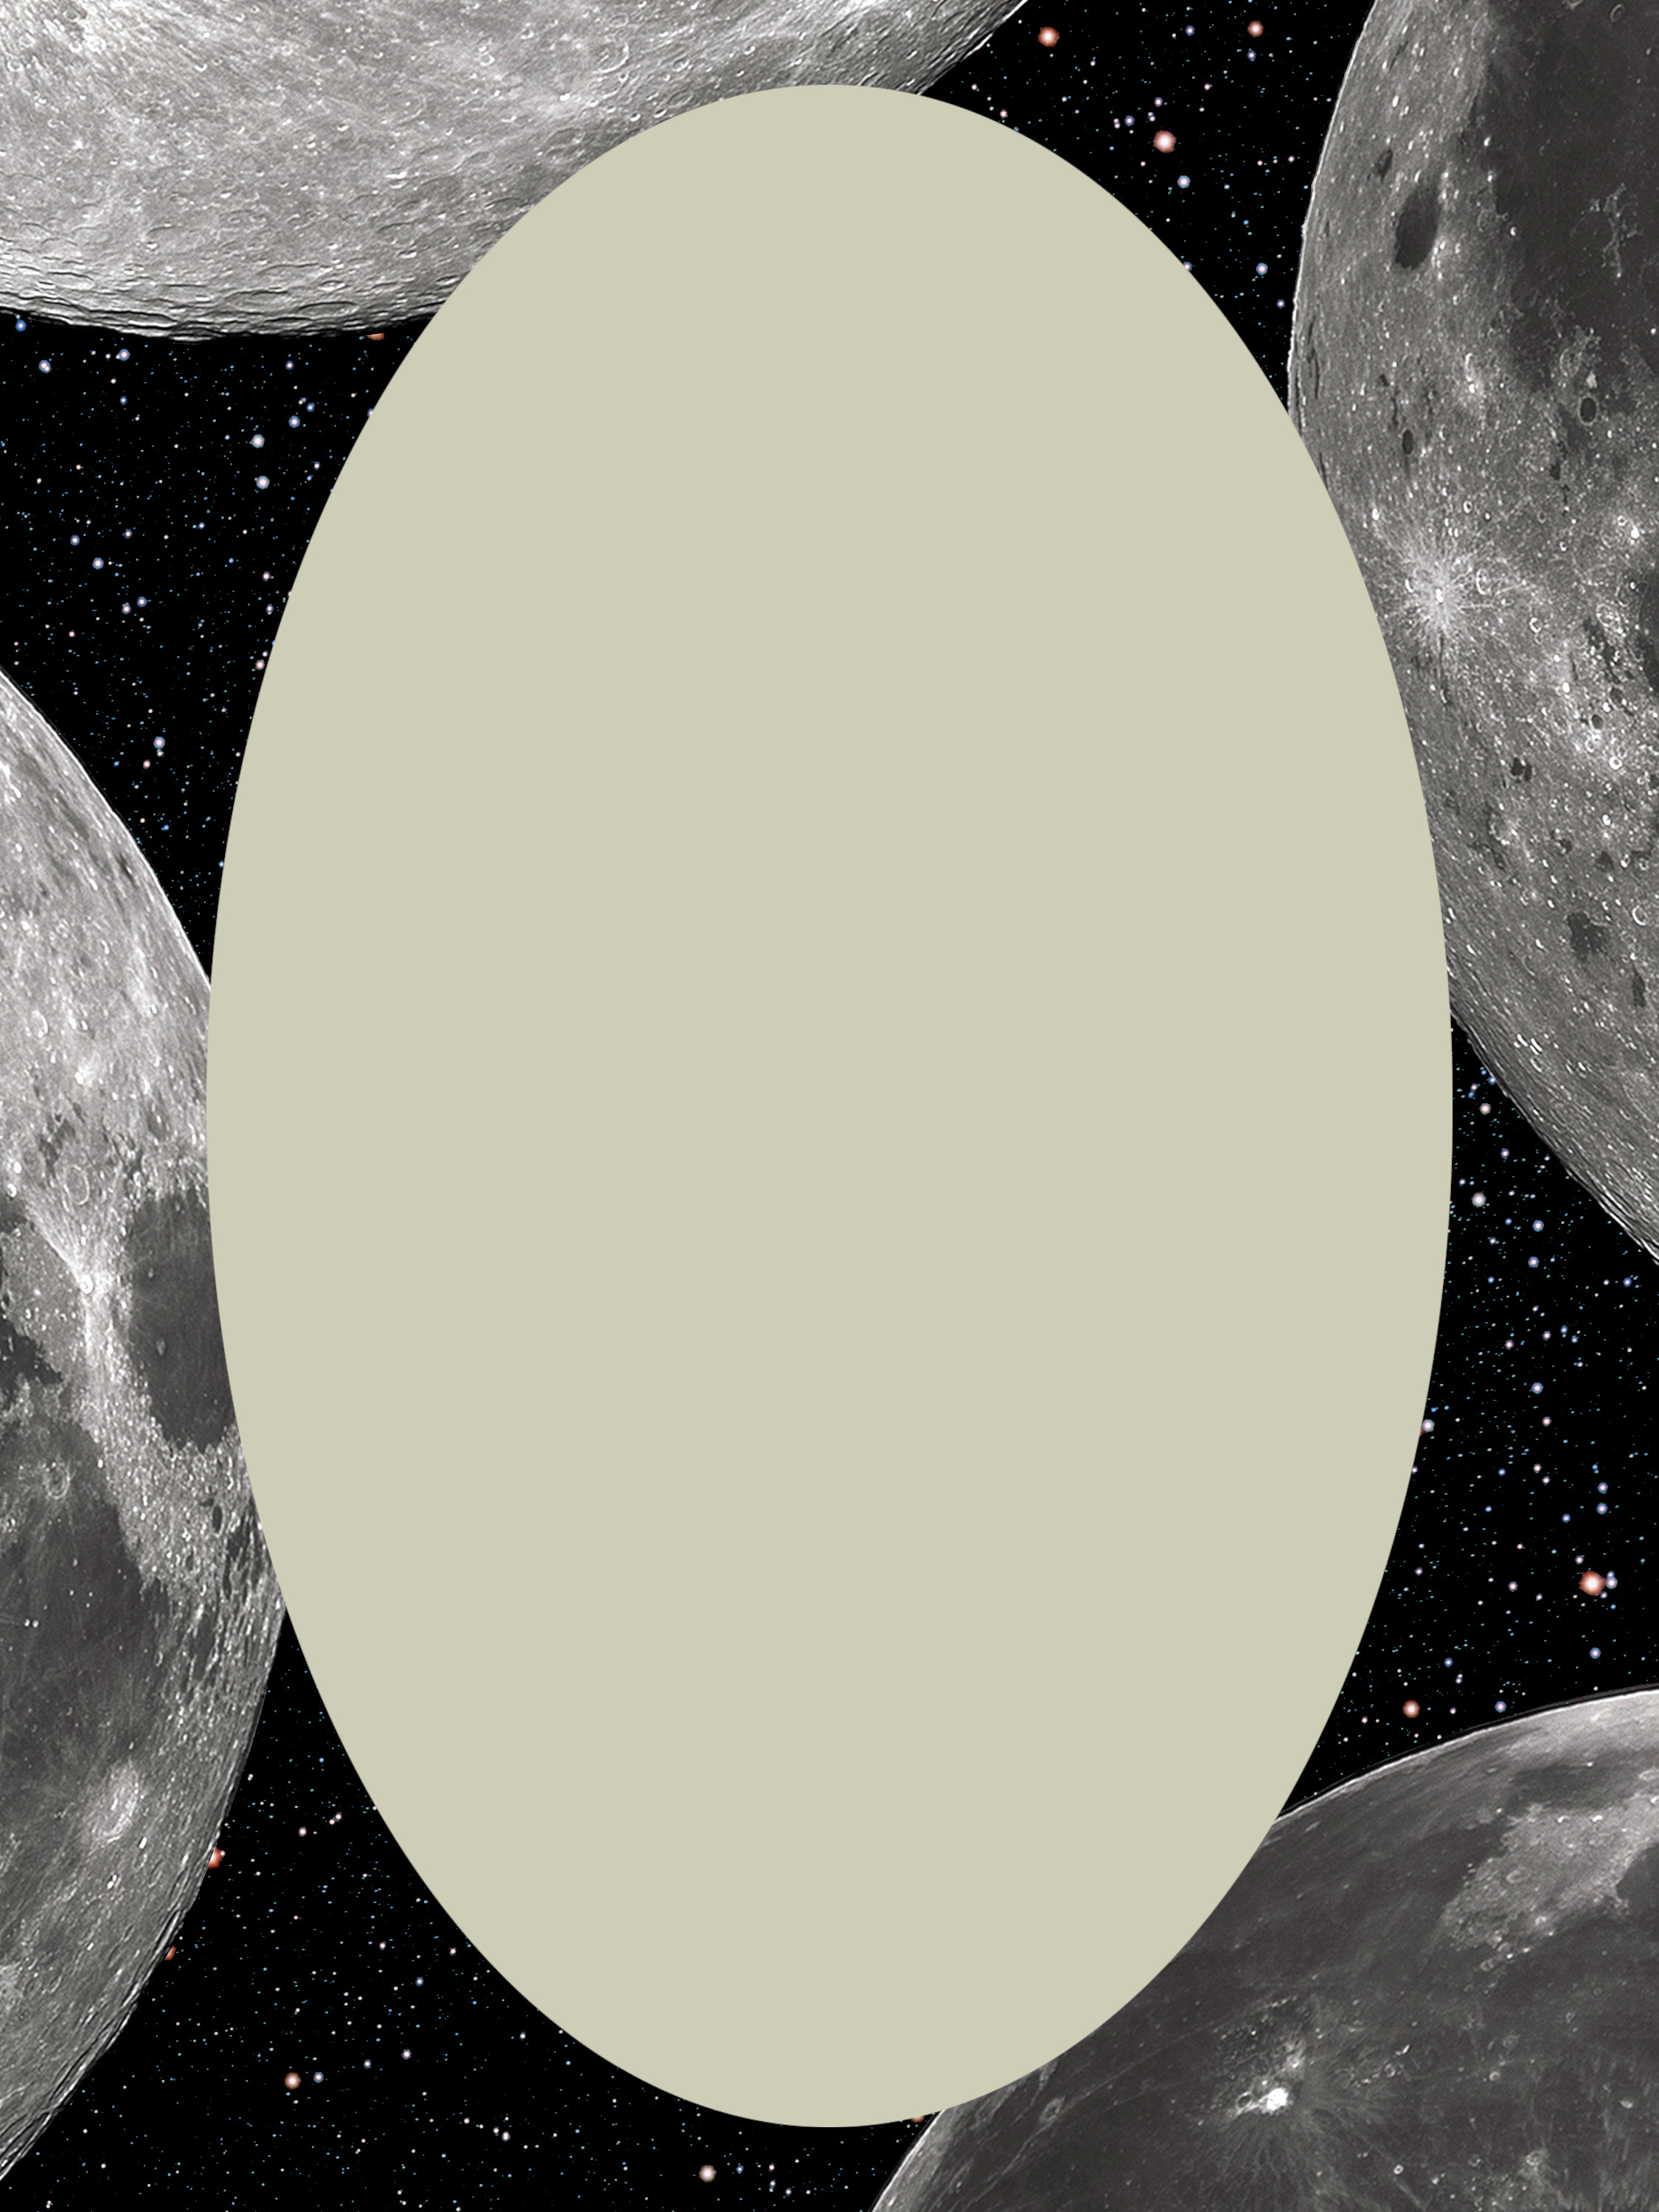
\includegraphics[width=\paperwidth,height=\paperheight]{moon-mist-large.jpeg}}
\begin{titlepage} % Suppresses headers and footers on the title page
	\centering % Centre everything on the title page
	%\scshape % Use small caps for all text on the title page

	%------------------------------------------------
	%	Title
	%------------------------------------------------

	\rule{\textwidth}{1.6pt}\vspace*{-\baselineskip}\vspace*{2pt} % Thick horizontal rule
	\rule{\textwidth}{0.4pt} % Thin horizontal rule
	
	\vspace{1\baselineskip} % Whitespace above the title
	
	{\Huge Περὶ τοῦ Ἐμφαινομένου \\ προσώπου τῷ κύκλῳ \\ τῆς Σελήνης}
	
	\vspace{1\baselineskip} % Whitespace above the title

	\rule{\textwidth}{0.4pt}\vspace*{-\baselineskip}\vspace{3.2pt} % Thin horizontal rule
	\rule{\textwidth}{1.6pt} % Thick horizontal rule
	
	\vspace{1\baselineskip} % Whitespace after the title block
	
	%------------------------------------------------
	%	Subtitle
	%------------------------------------------------
	
	{\Large Πλούταρχος}
 
        \vspace{0.5\baselineskip}
	
	\vspace*{1\baselineskip} % Whitespace under the subtitle
	
        {\scshape \normalsize } % Subtitle or further description

	%------------------------------------------------
	%	Editor(s)
	%------------------------------------------------
        \vspace*{\fill}    

	\vspace{1\baselineskip}

	{\small\scshape 1778}
	
	{\small\scshape{Impensis Gotthelf Theophil Georgi}}
	
	\vspace{0.5\baselineskip} % Whitespace after the title block

        {\scshape Internet Archive Online Edition}% Publication year}
    
	{\small CC Αναφορά-Μη Εμπορική Χρήση 4.0} % Publisher
\end{titlepage}
\setlength{\parskip}{1mm plus1mm minus1mm}
\clearpage
\large
%\tableofcontents
%\clearpage
\section[Περὶ τοῦ Ἐμφαινομένου προσώπου τῷ κύκλῳ τῆς Σελήνης]{Περὶ τοῦ Ἐμφαινομένου προσώπου τῷ κύκλῳ τῆς Σελήνης\footnote{Neque hic, neque alibi, ubi tot lacunae sunt, tot defectus, tot mendae, iniquus nobis esse debes, Lector, si tua, adeoque nostra etiam voluntate minus praestitimus. Nam neque affingere nostra Plutarco debuimus verba, quod non tam ostentationis est arrogantis, quam temeritatis insolentis: neque ipsius verba, codicum subsidio demto, restitui possunt. Spero tamen, quaedam impedimenta nos, solertibus coniecturis usos, summouisse, ut expeditior multo, atque antehac, huius libri tibi (quod idem in Symposiacis, Erotico, aliisque factum a nobis deprehendere potes) esse queat lectio, id quod te boni consulere par est, nos monuisse opus habuimus. \emph{Xylander.}}}
\paragraph{}
Ο μὲν τοὖν Σύλλας\footnote{Carere initio librum, quod est, esse ἀκέφαλον, non est obscurum: Syllae huius etiam in aliis libris est mentio nostri Plutarchi. \emph{Xylander.}} ταῦτα εἶπε. τῷ γὰρ ἐμῷ μύθῳ προσήκει, κᾀκεῖθέν ἐστιν. ἀλλὰ δεῖ τι πρὸς τὰς ἀνὰ χεῖρα ταύτας καὶ διὰ στόματος πᾶσι δόξας περὶ τοῦ προσώπου τῆς σελήνης προσανακρούσασθαι · πρῶτον ἡδὲως ἄν μοι δοκῶ πυθέσθαι. Τί δ ᾽ οὐκ ἐμέλλμεν (εἶπον) ὑπὸ τῆς ἐν τούτοις ἀπορίας ἐπ ᾽ ἐκείνους ἀπωσθέντες ; ὡς γὰρ οἱ ἐν νοσήμασι χρονίοις πρὸς τὰ κοινὰ βοηθήματα καὶ τὰς συνήθεις διαίτας ἀπειπόντες, ἐπὶ καθαρμοὺς καὶ περίαπτα καὶ ὀνείρους τρέπονται, οὕτως ἀναγκαῖον ἐν δυσθεωρήτοις καὶ ἀπόροις σκέψεσιν, ὅταν οἱ κοινοὶ καὶ ἔνδοξοι καὶ συνήθεις λόγοι μὴ πείθωσι, πειρᾶσθαι τῶν ἀτοπωτέρων, καὶ μὴ καταφρονεῖν, ἀλλ ᾽ ἐπᾴδειν ἀτεχνῶς ἑαυτοῖς τὰ τῶν παλαιῶν, καὶ διὰ πάντων τἀληθὲς ἐξελέγχειν. ὁρᾷς γὰρ εὐθὺς, ὡς ἄτοπος ὁ λέγων, τὸ φαινόμενον εἶδος\footnote{Ρrο τὸ Φαινόμενον εἶδος Turn. dat τὸ καλουμενον πρόσωπον.} ἐν τῇ σελήνῃ πάθος εἶναι τῆς ὄψεως, ὑπεικούσης τῇ λαμπρότητι δι ᾽ ἀσθένειαν, ὅ ... καλοῦμεν\footnote{ὃ $\star$ καλοῦμεν] Forte ὃ ἀμβλυώττειν καλοῦμεν. \emph{Xylander.} Ex Turn. affertur: ὅπερ ἀνάκλασιν, vel ἀνακλᾶσθαι, καλοῦμεν.} · οὐ συνορῶν, ὅτι πρὸς τὸν ἥλιον ἔδει τοῦτο γίνεσθαι μᾶλλον, ὀξὺν ἀπαντῶντα καὶ πλήκτην, ὥς που καὶ Ἐμπεδοκλῆς τὴν ἑκατέρων ἀποδίδωσιν οὐκ ἀηδῶς διαφοράν ·

Ἥλιος ὀξυμελης, ἠδὲ λάϊνα σελήνη\footnote{ἡ δὲ λάϊνα σελήνη] Versum corrigere vix ausim, etsi fortasse pro ἡ δὲ scriptum fuit a poëta ἡ δ ᾽ αὖ, vel ἠδ ᾽ αὖ: sed pro λάϊνα, minime dubium est, legendum esse Ἱλάειρα. [et sane Turn. et Vulc. dant ἡ δὲ ἱλάειρα] Lunae enim nomen est Ἱλάειρα, quod non Hesychius modo annotauit, sed etiam versus exstat Empedoclis in Simplicii in Aristotelis Physica commentariis:\\\hspace*{5mm}Ἡ δὲ Φλὸξ Ἱλάειρα μίνυνθα δίης τυχε γαίης.\\\hspace*{5mm}\emph{Obtigit et flammae lunari portio terrae.}\\\hspace*{5mm}Iam Apollodorus bibliothecae lib. 3. Phoeben et Ilairam Leucippi et Philodices, Inachi filiae, filias facit: quarum hanc Castor, illam Pollux duxerit uxorem: quod idem est apud Scholiasten Homeri Iliad. γ. ad versum 243. Atqui \emph{Phoeben} vocari Lunam notissimum est, minimeque fallit, poëtarum fabulis etiam astronomica fuisse antiquirus involuta. Quid quod Plutarchus ἐτυμολογῶν hoc loco, Lunae nomen παρὰ τὸ ἱλαρὸν deducit? Non ergo iam \emph{saxeam lunam}, sed \emph{renidentem et suaviter fulgentem}, habent lectores: restitutamque sibi Empedoclis sententiam: et ὀξυβελὴς suspicor, non ὀξυμελὴς, legendum. \emph{Xylander.} ὀξυβελὴς dant etiam Turn. et Vulc.} ·

τὸ ἐπαγωγὸν αὐτῆς καὶ ἱλαρὸν καὶ ἄλυπον οὕτω προσαγορεύσας. ἔπειτα λόγον ἀποδιδους, καθ ᾽ ὃν αἱ ἀμυδραὶ καὶ ἀσθενεῖς ὄψεις οὐδεμίαν διαφορὰν ἐν τῇ σελήνῃ μορφῆς ἐνορῶσιν, ἀλλὰ λεῖος αὐταῖς ἀντιλάμπει καὶ περίπλεως αὐτῆς ὁ κύκλος. οἱ δ ᾽ ὀξὺ καὶ σφοδρὸν ὁρῶντες, ἐξακριβοῦσι μᾶλλον, καὶ διαστέλλουσιν ἐκτυπούμενα τὰ εἴδη τοῦ προσώπου, καὶ τῆς διαφορᾶς ἅπτονται σαφέστερον. ἔδει γὰρ (οἶμαι) τοὐναντίον, εἴπερ ἡττωμένου τὰ\footnote{Ex Turn. affertur τοῦ ὂμματος.} ... ὄμματος ἐποίες τὴν φαντασίαν. ὅπου τὸ πάσχον ἀσθενέστερον εἶναι, τὸ φαινόμενον. ἡ δ ᾽ ἀνωμαλία καὶ παντάπασιν ἐλέγχει τὸν λόγον. οὐ γάρ ἐπὶ συνεχοῦς σκιᾶς καὶ συγκεχυμένης ὄψις. ἀλλ ᾽ οὐ φαύλως ὑπογράφων ὁ Ἀγησιάναξ\footnote{ὁ Ἡγησιάναξ Turn. et Vulc.} εἴρηκε ·

Πᾶσα μὲν ἥδε πέριξ πυρὶ λάμπεται, ἐν δ ᾽ ἄρα μέσσῃ ... Γλαυκότερον κυάνοιο φαείνεται ἠΰτε κοῦρος\footnote{In his versibus prο κοῦρος legi κούρης, et τὸ δ ᾽ ἄντα ἔοικεν ἐρεύθει: quanquam valde dubito de νοce ἐρεύθει. \emph{Xylander.} Prο κοῦρος Turn. et Vulc. dant κούρου.}

Ὄμμα, καὶ ὑγρὰ μέτωπα. τὸ δ ᾽ ἐρεύθει ἄντα ἔοικεν · ὄντως γὰρ ὑποδύεται περιόντα\footnote{περιϊόντα Turn. et Vulc.} τοῖς λαμπροῖς τὰ σκιερά. καὶ πιέζει πάλιν ὑπ ᾽ αὐτῶν καὶ ἀποκοπτόμενα · καὶ ὅλως πέπλεκται δι ᾽ ἀλλήλων · ... γραφκὴν τὴν δια ... εἶναι\footnote{Ex Turn. et Vulc. citatur: διαγραφικὴ νὴ Δία τοῦ σχήματος.} τοῦ σχήματος ... καὶ πρὸς Κλέαρχον,\footnote{Κλίαρχον Ald. Κλίταρχον Turn.} ὦ Ἀριστότελες, οὐκ ἀπιθάνως ἐδόκει λέγεσθαι τὸν ὑμέτερον. ὑμέτερος γὰρ ἀνὴρ ὁ Ἀριστοτέλης, τοῦ παλαιοῦ γεγονὼς συνήθης, εἰ καὶ πολλὰ τοῦ Περιπάτου παρέτρεψεν. ὑπολαβόντος δὲ τοῦ Ἀπολλωνιάδου τὸν λόγον, καὶ, τίς ἦν ἡ δόξα τοῦ Κλεάρχου, διαπυθομένου · Παντὶ μᾶλλον (ἔφην) ἀγνοεῖν, ἤ σοι, προσῆκόν ἐστι λόγον, ὥσπερ ἀφ ᾽ ἑστίας τῆς γεωμετρίας ὁρμώμενον. λέγει γὰρ ἀνὴρ, εἰκόνας ἐσοπτρικὰς εἶναι καὶ εἴδωλα τῆς μεγάλης θαλάσσης, ἐμφαινόμενα τῇ σελήνῃ τὸ καλούμενον πρόσωπον. ἥ τε γὰρ ἴτυς\footnote{Pro ἴτυς dant ὂψις Turn. et Vulc.} ἀνακλωμένη πολλαχόθεν ἅπτεσθαι τῶν οὐ κατ ᾽ εὐθυωρίαν ὁρωμένων πέφυκεν, ἥ τε πανσέληνος αὐτὴ πάντων ἐσόπτρων ὁμαλότητι καὶ στιλπνότητι κάλλιστόν ἐστι καὶ καθαρώτατον. ὥσπερ οὖν τὴν\footnote{ὥσπερ οὖν τὴν $\star$] Prο asteriscο sufficit ἶριν. \emph{Xylander.} Et hanc vοcem sane addunt Turn. et Vulc. e quorum posteriore affertur etiam πῆξιν prο ἶριν.} ... οἴεσθε ὑμεῖς ἀνακλωμένης ἐπὶ τὸν ἥλιον τῆς ὄψεως ἐνορᾶσθαι τῷ νέφει λαβόντι νοτερὰν ἡσυχῆ λειότητα καὶ ... ξιν,\footnote{Pro καὶ $\star$ ξιν potest legi καὶ σύντηξιν. \emph{Xylander.} Ex Turn. affertur καὶ τῆξιν, vel πῆξιν.} οὕτως ἐκεῖνος ἐνορᾶσθαι τῆ σελήνῃ τὴν ἔξω θάλασσαν, οὐκ ἐφ ᾽ ἧς ἐστι χώρας, ἀλλὰ ὅθεν ἡ κλάσις ἐποίησε τὴν ὄψιν,\footnote{τῆς ὄψεως Turn.} τὴν ἐπαφὴν αὑτῆς καὶ τὴν ἀνταύγειαν · ὥς που πάλιν ὁ Ἀγησιάναξ εἴρηκεν ·
\begin{quotation}\small
Ἢ πόντου μέγα κῦμα καταντία\footnote{κατ ᾽ ἀντία, duobus vocab. Turn. et Vulc.} κυμαίνοντος,

Δείκελον ἰνδάλλοιτο πυριφλεγέθοντος ἐσόπτρου.
\end{quotation}
\paragraph{}
πεισθεὶς\footnote{Pro πεισθεὶς Xylander vult legi ἡσθεὶς.} ὖν ὁ Ἀπολλωνίδης · Ὡς ἴδιον (εἶπε) καὶ καινὸν ὅλως τὸ σκευώρημα τῆς δόξης. τόλμαν δέ τινα καὶ μοῦσαν ἔχοντος ἀνδρός, ἀλλὰ πῆ\footnote{Pro πῆ Turn. et Vulc. dant σὺ, et pro προσῆγε, πρόσαγε.} τὸν ἔλεγχον αὐτῷ προσῆγε. Πρῶτον μὲν (εἶπον) εἰ\footnote{Pro εἰ Turn. exhibet ὅτι.} μία φύσις τῆς ἔξω θαλάσσης ἐστὶ, σύῤῥουν καὶ συνεχὲς πέλαγος, ἡ δ ᾽ εμφασις οὐ μία τῶν ἐν τῇ σελήνη μελασμάτων, ἀλλ ᾽ οἷον ἰσθμοὺς ἔχουσα, τοῦ λαμπροῦ διαιροῦντος καὶ διορίζοντος τὸ σκιερόν · ὅθεν ἐκάστου τόπου χωρισθέντος, καὶ πέρας ἴδιον ἔχοντος, αἱ τῶν φωτεινῶν ἐπιβολαὶ τοῖς σκοτεινοῖς ὕψους\footnote{ὕφους Ald. et Bas.} εἰκόνα καὶ βάθος λαμβάνουσαι τὰς περὶ τὰ ὄμματα καὶ τὰ χείλη εἰκόνας φαινομένας ὁμοιότατα διετύπωσαν · ὥστ ᾽ ἢ πλείονας ἔξω θαλάσσας ὑποληπτέον ἴσθμοῖς τισι καὶ ἠπείροις ἀπολαμβανομένας, ὅπερ ἐστὶν ἄτοπον καὶ ψεῦδος, ἢ μιᾶς οὔσης, οὐ πιθανὸν\footnote{πιθανὴν Ald. et Bas.} εἰκόνα διεσπασμένην οὕτως ἐμφαίνεσθαι. ἐκεῖνο μὲν γὰρ ἐρωτᾷν ἀσφαλέστερόν ἐστιν, ἢ ἀποφαίνεσθαι, σοῦ παρόντος, εἰ, τῆς οἰκουμένης εὖρος ἐχούσης\footnote{Pro ἐχούσης dant ἴσης Ald. et Bas.} καὶ μῆκος, ἐνδέχεται πᾶσαν ὡσαύτως ἀπὸ τῆς σελήνης ὄψιν ἀνακλωμένην ἐπιθιγγάνειν τῆς θαλάσσης καὶ τοῖς ἐν αὐτῇ μεγάλῃ θαλάττῃ πλέουσι νὴ Δία καὶ οἰκοῦσιν, ὥσπερ Βρεττανοῖς. καὶ ταῦτα μηδὲ τῆς γῆς, ὡς ἔφατε, πρὸς τὴν σφαῖραν τῆς σελήνης κέντρου λόγον ἐπεχούσης. Τουτὶ μὲν οὖν (ἔφην) σὸν ἔργον ἐπισκοπεῖν. τὴν δὲ πρὸς τὴν σελήνην ἢ τῆς ὄψεως κλάσιν, οὐκέτι σὸν, οὐδὲ Ἱππάρχου. καίτοι γε, φίλε πρίαμ\footnote{Φίλε πρίαμ. $\star$] Legendum videtur Φίλε Λαμπρία, πολλοῖς: et verti potuisse sine asterisco: \emph{Quanquam hic, mi Lampria, multis. Xylander.} Ex Turn. et Vulc. citatur Φίλε Πρίαμε, vel Λαμπρία.} ... ἀλλὰ πολλοῖς οὐκ ἀρέσκει φυσιολογῶν περὶ τῆς ὄψεως. αὐτὴν ὁμοπαθῆ\footnote{ἣν ὁμοιοπαθεῖν affertur ex Turn. et Vulc.} κρᾶσιν ἴσχειν καὶ σύμπηξιν εἰκός ἐστι μᾶλλον, ἢ πληγάς τινας καὶ ἀποπηδήσεις, οἵας ἔπλαττε τῶν ἀτόμων Ἐπίκουρος. οὐκ ἐθελήσει δὲ (οἶμαι) τὴν σελήνην ἐμβριθὲς ὑποθέσθαι σῶμα καὶ στερεὸν ὑμῖν ὁ Κλέαρχος, ἀλλ ᾽ ἄστρον αἰθέριον καὶ φωσφόρον, ὡς φατὲ,\footnote{Pro ὡς Φατὲ sententia videtur subiicere ᾧ οὐ Φατὲ. \emph{Xylander.}} τοιαύτη τὴν ὄψιν, ἢ θραῦσιν\footnote{θραύειν Turn. et Vulc.} προσήκει καὶ ἀποστρέφειν, ὥστ ᾽ οἴχεσθαι τὴν ἀνάκλασιν. εἰ δὲ προσδεῖταί τις ἡμᾶς, χρησόμεθα, πῶς μόνον πρόσωπόν ἐστιν ἐν τῇ σελήνῃ τὸ τῆς θαλάσσης ἔσοπτρον, ἄλλῳ δ ᾽ οὐδενὶ τῶν τοιούτων ἀστέρων ἐνορᾶται. καίτοι τό γ ᾽ εἰκὸς ἀπαιτεῖ, πρὸς ἅπαντας, ἢ πρὸς μηθένα τούτων, πάσχειν τὴν ὂψιν · ἀλλ ᾽ ... πρὸς τὸν Λεύκιον ἐφ ᾽ ὧν\footnote{Pro ἐφ ᾽ ὧν (ut videtur: non enim accurate indicatur, ad quam vocem haec lectio pertineat) dant εἶπον Turn. et Vulc.} ἀποβλέψας, ὃ πρῶτον ἐλέχθη τῶν ἡμετέρων, ὑπόμνησον. καὶ ὁ Λεύκιος · Ἀλλὰ μὴ δόξωμεν (ἔφη) κομιδῆ προπηλακίζειν τὸν Φαρνάκην, οὕτω τὴν Στωϊκὴν δόξαν ἀπροσάντητον ὑπερβαίνοντες, εἰπὶ δή τι πρὸς τὸν ἄνδρα, πάντως\footnote{παντὸς Ald. et Bas.} ἀέρος μίγμα καὶ μαλακοῦ πυρὸς ὑποτιθέμενον τὴν σελήνην, εἶτα οἷον ἐν γαλήνῃ φρίκης ὑποτρεχούσης φάσκοντα τοῦ ἀέρος διαμελαίνοντος ἔμφασιν γίνεσθαι μορφοειδῆ ... χρηστῶς γε (εἶπον) ὦ Λεύκιε, τὴν ἀτοπίαν εὐφήμοις περιαμπέχεις ὀνόμασιν. οὐχ οὕτω δὲ ὁ ἑταῖρος ἡμῶν, ἀλλ ᾽, ὅπερ ἀληθὲς ἦν, ἔλεγεν, ὑποπιέζειν αὐτοὺς τὴν σελήνην, σπίλων καὶ μελασμῶν ἀναπιμπλάντας, ὁμοῦ μὲν Ἄρτεμιν καὶ Ἀθηνὰν ἀνακαλοῦντας, ὁμοῦ δὲ σύμμιγμα\footnote{σύμμιγα Ald. et Bas.} καὶ φύραμα ποιοῦντας ἀέρος ζοφεροῦ καὶ πυρὸς ἀνθρακώδους, ουκ ἔχουσαν ἔξαψιν, οὐδ ᾽ αὐγὴν οἰκείαν, ἀλλὰ δυσκρινές τι σῶμα τυφόμενον ἀεὶ καὶ πυρίκαυστον · ὥσπερ τῶν κεραυνῶν τοὺς ἀλαμπεῖς καὶ ψολόεντας ὑπὸ τῶν ποιητῶν προσαγορευομένους. ὅτι μέντοι πῦρ ἀνθρακῶδες, οἷον οὗτοι τὸ τῆς σελήνης ποιοῦιν, οὐκ ἔχει διαμονὴν, οὐδὲ σύστασιν, ὅλως, ἐὰν μὴ στερεᾶς ὕλης καὶ στεγούσης ἅμα καὶ τρεφούσης ἐπιλάβηται, βέλτιον οἶμαι συνορᾷν ἐνίων φιλοσόφων τοὺς ἐν παιδιᾶ λέγοντας, τὸν Ἥφαιστον εἰρῆσθαι χωλὸν, ὅτι τὸ πῦρ ξύλων χωρὶς, ὥσπερ οἱ χωλοὶ βακτηρίας, οὐ πρόεισιν. εἰ οὖν ἡ σελήνη πῦρ ἐστι, πόθεν αὐτῇ τοσοῦτος ἐγγέγονεν ἀήρ · ὁ γὰρ ἄνω καὶ κύκλῳ φερόμενος οὑτοσὶ τόπος, οὐκ ἀέρος, ἀλλὰ κρείττονος οὐσίας, καὶ πάντα λεπτύνειν καὶ συνεξάπτειν φύσιν ἐχούσης ἐστίν. εἰ δὲ γέγονε, πῶς οὐκ οἴχεται μεταβάλλων εἰς ἕτερον εἶδος, ὑπὸ τοῦ πυρὸς ἐξαιθερωθεὶς, ἀλλὰ σώζεται, καὶ συνοικεῖ πυρὶ τοσοῦτον χρόνον, ὥσπερ ἧλος ἀραρὼς τοῖς αὐτοῖς ἀεὶ μέρεσι καὶ συγγεγομφωμένος. ἀραιῷ μὲν γὰρ ὄντι καὶ συγκεχυμένῳ μὴ μένειν, ἀλλὰ σφάλλεσθαι, προσήκει. συμπεπηγέναι δ ᾽ οὐ δυνατὸν ἀναμεμιγμένον πυρὶ, καὶ μήτε ὑγροῦ μετέχοντα, μήτε γῆς, οἷς μόνοις ἀὴρ συμπήγνυσθαι πέφυκεν. ἡ δὲ ῥύμη καὶ τὸν ἐν λίθοις ἀέρα, και τὸν ἐν ψυχρῷ μολίβδῳ, συνεκκᾴει · μήτι γε δὴ τὸν ἐν πυρὶ δινουμένῳ\footnote{δυνομένῳ Ald. et Bas. δινούμενον Turn. et Vulc.} μετὰ τάχους τοσούτου. καὶ γὰρ Ἐμπεδοκλεῖ δυσκολαίνουσι, πάγον ἀέρος χαλαζώδη ποιοῦντι τὴν σελήνην, ὑπὸ τῆς τοῦ πυρὸς σφαίρας περιεχόμενον. αὐτοὶ δὲ τὴν σελήνην, σφαῖραν οὖσαν πυρὸς, ἀέρα φασὶν ἄλλον ἄλλῃ διεσπασμένον περιέχειν, καὶ ταῦτα, μήτε ῥήξεις ἔχουσαν ἐν ἑαυτῇ, μήτε βάθη καὶ κοιλότητας, (ἅπερ οἱ γεώδη ποιοῦντες ἀπολείπουσιν) ἀλλὰ ἐπιπολῆς δηλονότι τῇ κυρτότητι ἐπικείμενον. τοῦτο δ ᾽ ἐστὶ καὶ πρὸς διαμονὴν ἄλογον, καὶ πρὸς θέαν ἀδύνατον ἐν ταῖς πανσελήνοις. διορίσασθαι γὰρ οὐκ ἔδει μέλανα καὶ σκιερὸν, ἀλλ ᾽ ἀμαυροῦσθαι κρυπτόμενον, ἢ συνεκλάμπειν, ὑπὸ τοῦ ἡλίου καταλαμβανομένης τῆς σελήνης. καὶ γὰρ παρ ᾽ ἡμῖν ὁ μὲν ἐν βάθεσι καὶ κοιλώμασι τῆς γῆς, οὗ μὴ δίεισιν αὐγὴ,\footnote{Pro αὐγὴ dant αὐτὴ Ald. et Bas.} διαμένει σκιώδης καὶ ἀφώτιστος · ὁ δ ᾽ ἔξωθεν τῇ γῇ περικεχυμένος, φέγγος ἴσχει καὶ χρόαν αὐγοειδῆ. πρὸς πᾶσαν μὲν γάρ ἐστι ποιότητα καὶ δύναμιν εὐκέραστος ὑπὸ μανότητος · μάλιστα δὲ φωτὸς ἂν ἐπιψαύσῃ μόνον, ὡς φατἐ, καὶ θίγῃ, διόλου τρεπόμενος ἐκφωτίζεται. ταὐτὸ οὖν τοῦτο καὶ τοῖς εἰς βάθη τινὰ καὶ φάραγγας συνωθοῦσιν ἐν τῇ σελήνῃ τὸν ἀέρα κἂν καλῶς ἔοικε βοηθεῖν, ὑμᾶς τε διεξελέγχει τοὺς ἐξ ἀέρος καὶ πυρὸς ούκ οἶδα ὅπως μιγνύντας αὐτῆς καὶ συναρμόζοντας τὴν σφαῖραν. οὐ γὰρ οἷόν τε λείπεσθαι σκιὰν ἐπὶ τῆς ἐπιφανείας, ὅταν ὁ ἥλιος ἐπιλάμπῃ τῷ φωτὶ πᾶν, ὁπόσον καὶ ἡμεῖς ἀποτεμνόμεθα τῇ ὄψει τῆς σελήνης. καὶ ὁ Φαρνάκης, ἔτι μοῦ λέγοντος · Τοῦτο ἐκεῖνο πάλιν (εἶπεν) ἐφ ᾽ ἡμᾶς ἀφῖκται τὸ περίακτον ἐκ τῆς Ἀκαδημίας, ἐν τῷ πρὸς ἑτέρους λέγειν, διατρίβοντας ἑκάστοτε μὴ παρέχειν ἔλεγχον, ὧν αὐτοὶ λέγουσιν · ἀλλ ᾽ ἀπολογουμένοις δεῖ χρῆσθαι, μὴ κατηγοροῦσιν ἂν ἐντυγχάνωσιν. ἐμὲ δ ᾽ οὖν οὐκ ἐξάξεσθε τήμερον εἰς τὸ διδόναι λόγον, ὧν ἐπικαλεῖτε τοῖς Στωϊκοῖς, πρὶν εὐθύνας λαβεῖν παρ ᾽ ὑμῶν, ἄνω τὰ κάτω τοῦ κόσμου ποιούντων. καὶ ὁ Λεύκιος γελάσας · Μόνον, (εἶπεν) ὦ τὰν, μὴ κρίσιν ἡμῖν ἀσεβείας ἐπαγγείλῃς. ὥσπερ Ἀρίσταρχος ᾤετο, δεῖν Κλεάνθη τὸν Σάμιον ἀσεβείας προκαλεῖσθαι τοὺς Ἕλληνας, ὡς κινοῦντα τοῦ κόσμου τὴν ἑστίαν, ὅτι φαινόμενα σώζειν ἀνὴρ ἐπειρᾶτο, μένειν τὸν οὐρανὸν ὑποτιθέμενος. ἐξελίττεσθαι δὲ κατὰ λοξοῦ κύκλου τὴν γῆν, ἅμα καὶ περὶ τὸν αὑτῆς ἄξονα δινουμένην. ἡμεῖς μὲν οὖν οὐδὲν αὐτοὶ παρ ᾽ αὑτῶν\footnote{περὶ αὐτῶν Turn.} λέγομεν. οἱ δὲ γῆν ὑποτιθέμενοι τὴν σελήνην, ὦ βέλτιστε, τί μᾶλλον ἡμῶν ἄνω τὰ κάτω ποιοῦσι, τὴν γῆν ἱδρυόντων ἐνταῦθα μετέωρον ἐν τῷ ἀέρι, πολλῷ τινι μείζονα τῆς σελήνης οὖσαν ; ὡς ἐν τοῖς ἐκλειπτικοῖς πάθεσιν οἱ μαθηματικοὶ καὶ ταῖς διὰ τοῦ σκιάματος παρόδοις τῆς ἐποχῆς τὸ μέγεθος ἀναμετροῦσιν. ἥ τε γὰρ σκιὰ τῆς γῆς ἐλάττων ὑπὸ μείζονος τοῦ φωτίζοντος ἀνατείνει, καὶ τῆς σκιᾶς αὐτῆς, λεπτὸν ὄντα\footnote{Pro ὄντα dant ὂν τὸ, duobus vocab. Turn. et Vulc.} ἄνω καὶ στενόν. οὐδ ᾽ Ὅμηρον, ὥς φησιν, ἔλαθεν, ἀλλὰ τὴν νύκτα θοὴν, ὀξύτητι τῆς σκιᾶς προσηγόρευσεν. ὑπὸ τούτου δ ᾽ ὅμως ἁλισκομένη ταῖς ἐκλείψεσιν ἡ σελήνη τρισὶ μόλις τοῖς αὑτῆς μεγέθεσιν ἀπαλλάττεται. σκόπει δὴ, πόσων ἡ γῆ σεληνῶν ἐστιν, εἰ σκιὰν ἀφίησιν, ἧς\footnote{ἧς abest ab Ald. et Bas.} ἡ βραχυτάτῃ πλάτος τρισέληνον. ἀλλ ᾽ ὅμως ὑπὲρ τῆς σελήνης, μὴ πέσῃ, δεδοίκατε. περὶ δὲ τῆς γῆς ἴσως Αἰσχύλος ὑμᾶς πέπεικεν, ὡς ὁ Ἄτλας
\begin{quotation}\small
Ἕστηκε, κίον ᾽ οὐρανοῦ τε καὶ χθονὸς

Ὤμοις ἐρείδων, ἄχθος οὐκ εὐάγκαλον.
\end{quotation}
\paragraph{}
εἰ τῇ μὲν σελήνῃ κοῦφος ἀὴρ ὑποτρέχει, καὶ στερεὸν ὄγκον οὐκ ἐχέγγυος ἐνεγκεῖν, τὴν δε γῆν κατὰ Πίνδαρον ἀδαμαντοπέδιλοι κίονες περιέχουσι. καὶ διὰ τοῦτο Φαρνάκης αὐτὸς μὲν ἐν ἀδείᾳ τοῦ πεσεῖν τὴν γῆν ἐστιν, οἰκτείρει δὲ τοὺς ὑποκειμένους τῇ μεταφορᾷ\footnote{καταφορᾷ Turn.} τῆς σελήνης Αἰθίοπας, ἢ Ταπροβηνοὺς, μὴ βάρος αὐτοῖς\footnote{αὐτῆς Ald.} ἐμπέσῃ τοσοῦτον. καίτοι τῇ μὲν σελήνῃ βοήθεια πρὸς τὸ μὴ πεσεῖν, ἡ κίνησις αὐτὴ, καὶ τὸ ῥιζῶδες τῆς περιαγωγῆς. ὥσπερ ὅσα ταῖς σφενδόναις ἐντεθέντα τῆς καταφορᾶς κώλυσιν ἴσχει τὴν κύκλῳ περιδίνησιν. ἄγει γὰρ ἕκαστον ἡ κατὰ φύσιν κίνησις, ἂν ὑπ ᾽ ἄλλου μηδενὸς ἀποστρέφηται. διὸ τὴν σελήνην οὐκ ἄγει τὸ βάρος, ὑπὸ τῆς περιφορᾶς τὴν ῥοπὴν ἐκκρουόμενον. ἀλλὰ μᾶλλον ἴσως λόγον εἶχε θαυμάζειν, μένουσαν αὐτὴν παντάπασιν, ὥσπερ ἡ γῆ, καὶ ἄτρεπτον.\footnote{Post ἄτρεπτον Turn. addit οὖσαν.} νῦν δὲ σελήνη μὲν ἔχει μεγάλην αἰτίαν τοῦ δεῦρο μὴ φέρεσθαι · τὴν δὲ γῆν, ἑτέρας κινήσεως ἄμοιρον οὖσαν, εἰκὸς ἦν μόνῳ τῷ βαρύνοντι μένειν.\footnote{Pro μένειν dant κινεῖν Ald. et Bas.} βαρυτέρα δέ ἐστι τῆς σελήνης, οὐχ ὅσῳ μείζων, ἀλλ ᾽ ἔτι μᾶλλον, ἅτε δὴ διὰ θερμότητα καὶ πύρωσιν ἐλαφρᾶς γεγενημένης ... ὅλως δ ᾽ ἔοικεν, ἐξ ὧν λέγεις, ἡ σελήνη μᾶλλον, εἰ πῦρ ἐστι, γῆς δεῖσθα καὶ ὕλης, ἐν ᾗ βέβηκε καὶ προσπέφυκε, καὶ συνέχει καὶ ζωπυρεῖ τὴν δύναμιν · οὐ γάρ ἐστι πῦρ χωρὶς ὕλης διανοηθῆναι σωζόμενον. γῆν δὲ φατὲ ὑμεῖς ἄνευ βάσεως καὶ ῥίζης διαμένειν. Πάνυ μὲν οὖν, (εἶπεν ὁ Φαρνάκης) τὸν οἰκεῖον καὶ κατὰ φύσιν τόπον ἔχουσαν, ὥσπερ αὐτὸ τὸ μέσον. οὗτος γάρ ἐστι, περὶ ὃν ἀντερείδει\footnote{ἀνερείδει Ald. et Bas.} πάντα τὰ βάρη ῥέποντα, καὶ φέρεται, καὶ συννεύει πανταχόθεν. ἡ δ ᾽ ἄνω χώρα πᾶσα, κᾄν τι δέξηται γεῶδες ὑπὸ βίας ἀναῤῥιφὲν, εὐθὺς ἐκθλίβει δεῦρο, μᾶλλον δ ᾽ ἀφίησιν, ᾗ πέφυκεν οἰκείᾳ ῥοπῇ καταφερόμενον. πρὸς τοῦτ ᾽ ἐγὼ τῷ Λευκίῳ χρόνον ἐγγενέσθαι βουλόμενος ἀναμιμνησκομένῳ, τὸν Θέωνα καλέσας · Τίς, (ἔφην) ὦ Θέων, εἴρηκε τῶν τραγικῶν, ὡς ἰατροὶ πικρὰν πικροῖς κλύζουσι φαρμάκοις χολήν ; ἀποκριναμένου δὲ τοῦ Θέωνος, ὅτι Σοφοκλῆς · Καὶ δοτέον (εἶπον) ὑπ ᾽ ἀνάγκης ἐκείνοις · φιλοσόφων δ ᾽ οὐκ ἀκουστέον, ἂν τὰ παράδοξα παραδόξοις ἀμύνεσθαι βούλωνται, καὶ μαχόμενοι πρὸς τὰ θαυμάσια τῶν δογμάτων, ἀτοπώτερα καὶ θαυμασιώτερα πλάττωσιν, ὥσπερ οὗτοι τὴν ἐπὶ τὸ μέσον φορὰν εἰσάγουσιν. ᾗ τί παράδοξον οὐκ ἔνεστιν ; οὐχὶ τὴν γῆν σφαῖραν εἶναι, τηλικαῦτα βάθη καὶ ὕψη καὶ ἀνωμαλίας ἔχουσαν ; οὐκ ἀντίποδας οἰκεῖν, ὥσπερ θρίπας, ἢ γαλεώτας, τραπέντα ἄνω τὰ κάτω τῇ γῇ προϊσχομένους ; ἡμᾶς δ ᾽ αὐτοὺς μὴ πρὸς ὀρθὰς βεβηκότας, ἀλλὰ πλαγίους ἐπιμένειν ἀπονεύοντας, ὥσπερ οἱ μεθύοντες ; οὐ μύδρους χιλιοταλάντους διὰ βάθους τῆς γῆς φερομένους, ὅταν ἐξίκωνται πρὸς τὸ μέσον, ἵστασθαι, μηδενὸς ἀπαντῶντος, μηδὲ ὑπερείδοντος ; εἰ δὲ ῥύμῃ κάτω φερομένου τὸ μέσον ὑπερβάλλοιεν, αὖθις ὀπίσω στρέφεσθαι καὶ ἀναπλάττειν\footnote{ἀναπλήττειν Bas. ἀναπίπτειν Turn. et Vulc. e quorum priore, Turn. affertur etiam ἀναπάλεσθαι: forte voluit ἀναπάλλεσθαι.} ἀπ ᾽ αύτῶν ; οὐ τμήματα δοκῶν ἀποπρισθέντα τῆς γῆς ἑκατέρωθεν μὴ φέρεσθαὶ κάτω διαπαντὸς, ἀλλὰ προσπίπτοντα πρὸς τὴν γῆν ἔξωθεν ἴσως διωθεῖσθαι καὶ ἀποκρύπτεσθαι περὶ τὸ μέσον ; οὐ ῥεῦμα λάβρον ὕδατος κάτω φερόμενον, εἰ πρὸς τὸ μέσον ἔλθοι σημεῖον, ὅπερ αὐτοὶ λέγουσιν ἀσώματον, ἵστασθαι περικεραννύμενον κύκλῳ περὶ πόλον ἄπαυστον αἰώραν καὶ ἀκατάπαυστον αἰωρούμενον. οὐδὲ γὰρ ψευδῶς ἔνια τούτων βιάσαιτο ἄν τις αὐτὸν εἰς τὸ δυνατὸν τῇ ἐπινοίᾳ καταστῆσαι. τοῦτο γάρ ἐστι τὰ ἄνω, κάτω · κἂν πάντα τραπέντα πάλιν εἶναι τῶν ἄχρι τοῦ μέσου κάτω, τῶν δὲ ὑπὸ τὸ μέσον, αὖ πάλιν ἄνω γενομένων. ὥστ ᾽, εἴ τις συμπαθείᾳ\footnote{εὐβαθείᾳ Turn.} τῆς γῆς τὸ μέσον αὐτῆς ἔχων σταίη περὶ τὸν ὀμφαλὸν ἅμα καὶ τὴν κεφαλὴν ἄνω, καὶ τοὺς πόδας ἄνω ἔχειν τὸν αὐτὸν, κἂν μὴ διασκάπτῃ τὸν ἐπέκεινα τόπον ἀνακύπτον αὐτοῦ το\footnote{Ex Turn. et Vulc. citatur αὐτοῦ τὸ μέρος ἄνω.} ... εἶναι καὶ κάτω ἄνωθεν ἕλκεσθαι τὸν ἀνασκαπτόμενον. εἰ δὲ δὴ τούτῳ τὶς ἀντιβεβηκὼς νοοῖτο, τοὺς ἀμφοτέρων ἅμα πόδας ἄνω γίνεσθαι καὶ λέγεσθαι. τοιούτων μέντοι καὶ τοστούτων παραδόξων λόγων\footnote{λογιῶν Ald. et Bas.} οὐ μὰ Δία πεῖραν, ἀλλὰ θαυματοποιοῦ τινος ἀποσκευὴν καὶ πυλαίαν κατανωτισάμενοι καὶ παρέλκοντες ἑτέρους φασὶ πελάζειν\footnote{γελοιάζειν Turn.} ἄνω τὴν σελήνην, γῆν οὖσαν, ἐνιδρύοντες οὐχ ὅπου τὸ μέσον ἐστί. καίτοι γε εἰ πᾶν σῶμα ἐμβριθὲς εἰς τὸ αὐτὸ συννεύει, καὶ πρὸς τὸ αὐτοῦ μέσον ἀντερείδει πᾶσι τοῖς μορίοις, οὐχ ὡς μέσον οὖσα τοῦ παντὸς ἡ γῆ μᾶλλον, ἢ ὡς ὅλον, οἰκειώσεται μέρη αὐτῆς ὄντα τὰ βάρη, καὶ τεκμήριον ... ἔσται τῶν ῥεπόντων, οὐ τῇ τῆς μεσότητος πρὸς τὸν κόσμον, ἀλλὰ πρὸς τὴν γῆν κοινωνίας πρὸς καὶ συμφυΐας τοῖς ἀποσπωμένοις αὐτῆς,\footnote{ἀπωσμένοις αὐτοῖς Ald. et Bas.} εἶτα πάλιν καταφερομένοις. ὡς γὰρ ὁ ἥλιος εἰς ἑαυτὸν ἐπιστρέφει τὰ μέρη, ἐξ ὧν συνέστηκε, καὶ ἡ γῆ τὸν λίθον, ὥσπερ ... προσήκοντα δέχεται, καὶ φέρει πρὸς ἐκεῖνον. ὅθεν ἑνοῦται τῷ χρόνω καὶ\footnote{καὶ abest ab Ald. et Bas.} συμφύεται πρὸς αὐτὴν τῶν τοιούτων ἕκαστον. εἰ δέ τι τυ γχάνει σῶμα τῇ γῇ μὴ προσνενεμημένον ἀπ ᾽ ἀρχῆς, μηδ ᾽ ἀπεσπασμένον, ἀλλά που\footnote{ἀλλὰ τοῦ Ald. et Bas.} καθ ᾽ αὑτὸ σύστασιν ἔσχεν ἰδίαν καὶ φύσιν, ὡς φαῖεν ἂν ἐκεῖνοι τὴν σελήνην, τί κωλύει χωρὶς εἶναι καὶ μένειν περὶ αὐτὸ, τοῖς αὐτοῦ πεπιεσμένον μέρεσι καὶ συμπεπεδημένον · οὔτε γὰρ ἡ γῆ μέσον οὖσα δείκνυται τοῦ παντὸς, ἥ τε πρὸς τὴν γῆν τῶν ἐνταῦθα συναίρεσις καὶ σύστασις ὑφηγεῖται τὸν τρόπον, ᾧ μένειν τὰ ἐκεῖ συμπεσόντα πρὸς τὴν σελήνην εἰκός ἐστιν. ὁ δὲ πάντα τὰ γεώδη καὶ βαρέα συνελαύνων εἰς μίαν χώραν, καὶ μέρη ποιῶν ἑνὸς σώματος, οὐχ ὁρῶ, διὰ τί τοῖς κούφοις τὴν αὐτὴν ἀνάγκην οὐκ ἀνταποδίδωσιν, ἀλλ ᾽ ἐᾷ χωρὶς εἶναι συστάσεις πυρὸς τοσαύτας, καὶ οὐ πάντας εἰς τοῦτο συνάγων τοὺς ἀστέρας σαφῶς\footnote{Pro σαφῶς dant ἃφῶς Turn. et Vulc. et paulo inferius post εἶναι iidem inserunt καὶ.} οἴεται δεῖν καὶ σῶμα κοινὸν εἶναι τῶν ἄνω φορῶν\footnote{Pro τῶν ἄνω φορῶν Ald. et Bas. dant τῶν ἀναφορῶν, unde Xylander ita annotat: τῶν ἀναφορῶν] Hanc vocem non probo, reponendumque suspicor ἀνωφερῶν: quale mendum alibi quoque notavimus.} καὶ φλογοειδῶν ἁπάντων · ἀλλ ᾽ ἥλιον μὲν ἀπλέτους μυριάδας ἀπέχειν τῆς ἄνω περιφορᾶς, φατὲ, εἶπεν,\footnote{Pro εἶπεν legendum est εἶπον. \emph{Xylander.}} ὦ φίλε Ἀπολλωνίδη, καὶ Φωσφόρον ἐπ ᾽ αὐτῷ, καὶ Στίλβοντα, καὶ τοὺς ἄλλους πλανήτας, ὑφιεμένους τε τῶν ἀπλανῶν, καὶ πρὸς ἀνέμους\footnote{Pro πρὸς ἀνέμους legendum πρὸς ἀλλήλους. Nihil enim hic ventis opus est. \emph{Xylander.} Turn. ac Vulc. dant πρὸς ἑαυτοὺς.} ἐν διαστάσεσι μεγάλαις φέρεσθαι · τοῖς δὲ βαρέσι\footnote{βαθέσι Ald.} καὶ γεώδεσιν οὐδεμίαν οἴεσθαι τὸν κόσμον εὐρυχωρίαν παρέχειν ἐν ἑαυτῶ καὶ διάστασιν. ὁρᾶτε, ὅτι γελοῖόν ἐστιν, εἰ γῆν οὐ φήσομεν εἶναι τὴν σελήνην, ὅτι τῆς κάτω χώρας ἀφέστηκεν, ἄστρον δὲ φήσομεν, ὁρῶντες ἀπωσμένην τῆς ἄνω περιφορᾶς μυριάσι σταδίων τοσαύταις, ὥσπερ βυθόν τινα καταδεδυκυῖαν. τῶν μέν γ ᾽ ἀστρων κατωτέρω τοσοῦτόν ἐστιν, ὅσον οὐκ ἄν τις εἴποι μέτρον, ἀλλ ᾽ ἐπιλείπουσιν ἡμᾶς τοὺς μαθηματικοὺς ἐκλογιζομένους οἱ ἀριθμοί. τῆς δὲ γῆς τρόπον τινὰ ψαύει καὶ περιφερομένη πλησίον, ἅρματος ὥσπερ ἴχνος, ἀνελίσσεται, φησὶν Ἐμπεδοκλῆς, ἥ τε περὶ ἄκραν.\footnote{παρ ᾽ ἂκραν Turn.}

οὐδὲ γὰρ τὴν σκιὰν αὐτῆς ὑπερβάλλει πολλάκις ἐπὶ μικρὸν αἰρομένη, τῷ παμμέγεθες εἶναι τὸ φωτίζον · ἀλλ ᾽ οὕτως ἔοικεν ἐν χρῷ καὶ σχεδὸν ἐν ἀγκάλαις τῆς γῆς περιπολεῖν, ὥστ ᾽ ἀντιφράττεσθαι πρὸς τὸν ἥλιον ὑπ ᾽ αὐτῆς, μὴ ὑπεραίρουσα τὸν σκιερὸν καὶ χθόνιον καὶ νυκτερινὸν τοῦτον τόπον, ὃς γῆς κλῆρός ἐστι. διὸ λεκτέον οἶμαι θαῤῥοῦντας, ἐν τοῖς τῆς γῆς ὅροις εἶναι σελήνην ὑπὸ τῶν ἄκρων αὐτῆς ἐπιπροσθουμένην. σκόπει δὲ τοὺς ἄλλους ἀφεὶς ἀπλανεῖς καὶ πλανήτας, ἃ δείκνυσιν Ἀρίσταρχος ἐν τῷ περὶ μεγεθῶν καὶ ἀποστημάτων, ὅτιτὸτοῦ ἡλίου ἀπόστημα τοῦ ἀποστήματος τῆς σελήνης, ὃ ἀφέστηκεν ἡμῶν πλέον μὲν, ἢ ὀκτωκαιδεκαπλάσιον, ἔλαττον δὲ, ἢ εἰκοσαπλάσιον, ἐστί. καίτοι ὁ τὴν σελήνην ἐπιμήκιστον αἴρων, ἀπέχει (φησὶ\footnote{ἀπέχειν φησὶν Turn.}) ἡμῶν ἓξ καὶ πεντηκονταπλάσιον τῆς ἐκ τοῦ κέντρου τῆς γῆς. αὕτη δ ᾽ ἐστὶ τεσσάρων μυριάδων. καὶ κατὰ τοὺς μέσως ἀναμετροῦντας, καὶ ἀπὸ ταύτης συλλογιζομένους, ἀπέχει ὁ ἥλιος τῆς σελήνης πλέον, ἢ τετρακισχιλίας τριάκοντα μυριάδας. οὕτως ἀπώκισται τοῦ ἡλίου διὰ βάρος, καὶ τοσοῦτο τῇ γῇ προσκεχώρηκεν. ὥστε, εἰ τότε\footnote{εἴ ποτε Turn. et Vulc.} τόποις τὰς οὐσίας διαιρετέον, ἡ γῆς μοῖρα καὶ ὥρα\footnote{χώρα iidem.} προσκαλεῖται σελήνην, καὶ τοῖς περὶ γῆν πράγμασι καὶ σώμασιν ἐπίδικός ἐστι κατ ᾽ ἀγχιστείαν καὶ γειτνίασιν. καὶ οὐθὲν (οἶμαι) πλημμελοῦμεν, ὅτι τοῖς ἄνω προσαγορευομένοις βάθος τοσοῦτον καὶ διάστημα διδόντες ἀπολείπωμέν τινα καὶ τῷ κάτω περιδρομὴν καὶ πλάτος, ὅσον ἐστὶν ἀπὸ γῆς ἐπὶ σελήνην. οὔτε γὰρ ὁ τὴν ἄκραν ἐπιφάνειαν τοῦ οὐρανοῦ μόνην ἄνω, τἄλλα δὲ κάτω προσαγορεύων ἅπαντα, μέτριός ἐστιν · οὔτε ὁ τῇ γῇ, μᾶλλον δὲ ὁ τῷ κέντρῳ\footnote{μέτρῳ Ald. et Bas.} τὸ κάτω περι γράφων ἀνεκτὸς, ἀλλὰ καὶ κινητικο ... ταύτῃ διάστημα τὸ δέον ἐπιχωροῦντος τοῦ κόσμου διὰ μέγεθος. πρὸς δὲ τὸν ἀξιοῦντα, πᾶν εὐθὺς ἄνω καὶ μετέωρον εἶναι τὸ ἀπὸ τῆς γῆς, ἕτερος ἀντηχεῖ πάλιν, εὐθὺς εἶναι κάτω τὸ ἀπὸ τῆς ἀπλανοῦς περιφορᾶς. ὅλως δὲ πῶς λέγεται, καὶ τίνος ἡ γῆ μέση κεῖται ; τὸ γὰρ πᾶν ἄπειρόν ἐστι. τῷ δ ᾽ ἀπείρῳ, μήτ ᾽ ἀρχὴν ἔχοντι, μήτε πέρας, οὐ προσήκει μέσον ἔχειν. πέρας γάρ τι καὶ τὸ μέσον · ἡ δ ᾽ ἀπειρία, περάτων στέρησις. ὁ δὲ μὴ τοῦ παντὸς, ἀλλὰ τοῦ κόσμου, μέσην εἶναι τὴν γῆν ἀποφαινόμενος ἡδύς ἐστιν, εἰ μὴ καὶ τὸν κόσμον αὐτὸν ἐνέχεσθαι ταῖς αὐταῖς ἀπορίαις νομίζει. τὸ γὰρ πᾶν, οὐδὲ τούτῳ μέσην\footnote{τοῦτο μέσην Ald. et Bas. τοῦτον μέσον Turn. et Vulc.} ἀπέλιπεν, ἀλλ ᾽ ἀνέστιος καὶ ἀνίδρυτός ἐστιν ἐν ἀπείρῳ κενῷ φερόμενος πρὸς οὐδὲν οἰκεῖον, εἰ\footnote{Pro εἰ dant ἢ Turn. et Vulc.} ἄλλην τινὰ τοῦ μένειν αἰτίαν εὑράμενος ἕστηκεν, οὐ κατὰ τὴν τοῦ τόπου φύσιν. ὅμοια καὶ περὶ σελήνης εἰκάζειν τινὶ πάρεστιν ὡς ἑτέρα τινὶ ψυχῇ καὶ φύσει μᾶλλον ... διαφοραὶ, τῆς μὲν ἀτρεμούσης ἐνταῦθα, τῆς δὲ καὶ φερομένης. ἄνευ δὲ τούτων, ὅρα, μὴ μέγα τι λέληθεν αὐτούς. εἰ γὰρ ὁποσονοῦν καὶ ὅτι ἂν ἐκτὸς γένηται τοῦ κέντρου τῆς γῆς ἄνω ἐστὶν, οὐθέν ἐστι τοῦ κόσμου κάτω μέρος. ἀλλ ᾽ ἄνω καὶ ἡ γῆ καὶ τὰ ἐπὶ γῆς, καὶ πᾶν ἁπλῶς σῶμα τὸ κέντρῳ περιεστηκὸς, ἢ περικείμενον, ἄνω γίνεται, κάτω δὲ μόνον ὂν ἓν, τὸ ἀσώματον σημεῖον ἐκεῖνο, ὃ πρὸς πᾶσαν ἀντικεῖσθαι τὴν τοῦ κόσμου φύσιν ἀναγκαῖον, εἴγε δὴ τὸ κάτω πρὸς τὸ ἄνω κατὰ φύσιν ἀντίκειται. καὶ οὐ τοῦτο μόνον τὸ ἄτοπον, ἀλλὰ καὶ τὴν αἰτίαν ἀπόλλυσι τὰ βάρη, δι ᾽ ἣν δεῦρο καταῤῥέπει καὶ φέρεται. σῶμα μὲν γὰρ οὐθέν ἐστι κάτω, πρὸς ὃ κινεῖται · τὸ δ ᾽ ἀσώματον, οὔτ ᾽ εἰκὸς, οὔτε βούλονται τοσαύτην ἔχειν δύναμιν, ὥστε πάντα κατατείνειν ἐφ ᾽ ἑαυτὸ, καὶ περὶ αὐτὸ συνέχειν. ἀλλ ᾽ ὅμως ἄλογον εὑρίσκεται καὶ μαχόμενον τοῖς πράγμασι, τὸ ἄνω τὸν κόσμον ὅλον εἶναι, τὸ δὲ κάτω μηθὲν, ἀλλ ᾽ ἢ πέρας ἀσώματον καὶ ἀδιάστατον. ἐκεῖνο δ ᾽ εὔλογον, ὡς λέγομεν ἡμεῖς, τῷ τ ᾽ ἄνω χώραν καὶ τῷ κάτω πολλὴν καὶ πλάτος ἔχουσαν διῃρῆσθαι. οὐ μὴν ἀλλὰ θέντες, (εἰ βούλει) παρὰ φύσιν ἐν οὐρανῷ τοῖς γεώδεσι τὰς κινήσεις ὑπάρχειν, ἀτρέμα, μὴ τραγικῶς, ἀλλὰ πρᾴως, σκοπῶμεν, ὅτι τοῦτο τὴν σελήνην οὐ δείκνυσι γῆν μὴ οὖσαν, ἀλλὰ γῆν, ὅπου μὴ πέφυκεν, οὖσαν. ἐπεὶ καὶ τὸ πῦρ τὸ Λἰτναῖον ὑπὸ γῆν παρὰ φύσιν ἐστὶν, ἀλλὰ πῦρ ἐστι · καὶ τὸ πνεῦμα τοῖς ἀσκοῖς περιληφθὲν, ἔστι μὲν ἀνωφερὲς φύσει καὶ κοῦφον, ἥκειδὲ, ὅπου μὴ πέφυκεν, ὑπ ᾽ ἀνάγκης. αὐτὴ δὲ ἡ ψυχὴ πρὸς Διὸς (εἶπεν) οὐ παρὰ φύσιν τῷ σώματι συνεῖρκται βραδεῖ ταχεῖα, καὶ ψυχρῷ πυρώδης, ὥσπερ ὑμεῖς φατὲ, καὶ ἀόρατος αἰσθητῷ. διὰ τοῦτο οὖν σώματι ψυχὴν μὴ λέγομεν εἶναι μηδὲν, οὐ\footnote{Pro μηδὲν, οὐ dant μηδενὶ, uno vocab. Turn. et Vulc.} χρῆμα θεῖον ὑπὸ βρίθους, ἢ πάχους, οὐρανόν τε πάντα καὶ γῆν καὶ θάλασσαν ἐν ταυτῷ περιπολοῦντα, καὶ διϊστάμενον εἰς σάρκας ἥκειν καὶ νεῦρα καὶ μυελοὺς, καὶ παθέων μυρίων μετὰ ὑγρότητος. ὁ δὲ Ζεὺς ἡμῖν οὗτος, οὐ τῇ μὲν αὐτοῦ φύσει χρώμενος ἔνεστι\footnote{Pro ἔνεστι codex Turn. dat ἕν ἐστι, duobus vocabulis.} μέγα πῦρ καὶ συνεχὲς, νυνὶ δὲ ὑφεῖται καὶ κέκαμπται, καὶ διεσχημάτισται, πᾶν χρῆμα\footnote{χρῶμα Ald. et Bas.} γεγονὼς καὶ γινόμενος ἐν ταῖς μεταβολαῖς ; ὥστε ὅρα καὶ σκόπει, δαιμόνιε, μὴ μεθιστὰς καὶ ἀπάγων ἕκαστον, ὅπου πέφυκεν εἶναι, διάλυσίν τινα κόσμου φιλοσοφῇς, καὶ τὸ νεῖκος ἐπάγῃς τὸ Ἐμπεδοκλέους τοῖς πράγμασι · μᾶλλον δὲ τοὺς παλαιοὺς κινῇς τιτᾶνας ἐπὶ τὴν φύσιν, καὶ γίγαντας καὶ τὴν μυθικὴν ἐκείνην καὶ φοβερὰν ἀκοσμίαν καὶ πλημμέλειαν ἐπιδεῖν πονῇς,\footnote{ποινῆς Turn.} χωρὶς τὸ βαρὺ πᾶν, καὶ χωρὶς\footnote{Ex eodem Turn. affertur πᾶν τὸ κοῦφον, unde incertum est, absintne [?] haec duo vocab. καὶ χωρὶς, ab hoc codice, an vero πᾶν post illa iteratum sit, quod accuratius indicari debebat.}
\begin{quotation}\small
τὸ κοῦφον,

Ἔνθ ᾽ οὔτ ᾽ ἠελίοιο δεδίττεται ἀγλαὸν εἶδος,

Οὐ δέμεν οὐδ ᾽ αἴης λάσιον γένος, οὐδὲ θάλασσα,
\end{quotation}
\paragraph{}
ὥς φησιν Ἐμπεδοκλῆς, οὐ γῆ θερμότητος μετεῖχεν, οὐχ ὕδωρ πνεύματος, οὐκ ἄνω τὶ τῶν βαρέων, οὐ κάτω τὶτῶν κούφων, ἀλλ ᾽ ἄκρατοι καὶ ἄστοργοι καὶ μονάδες αἱ τῶν ὅλων ἀρχαὶ, μὴ προσιέμεναι σύγκρισιν ἑτέρου πρὸς ἕτερον, μηδὲ κοινωνίαν, ἀλλὰ φεύγουσαι καὶ ἀποστρεφόμεναι, καὶ φερόμεναι φορὰς ἰδίας καὶ αὐθάδεις, οὕτως εἶχον, ὡς ἔχει πᾶν, οὗ θεὲς ἄπεστι κατὰ Πλάτωνα, τουτέστιν, ὡς ἔχει τὰ σώματα, νοῦ καὶ ψυχῆς ἀπολιπούσης · ἄχρις οὗ τὸ ἱμερτὸν ἧκεν ἐπὶ τὴν φύσιν ἐκ\footnote{ἐκ abest a Bas. ex Ald. autem citatur vox corrupta, ἀπρονοίας.} προνοίας, φιλότητος ἐγγενομένης, καὶ Ἀφροδίτης, καὶ Ἔρωτος, ὡς Ἐμπεδοκλῆς λέγει, καὶ Παρμενίδης, καὶ Ἡσίοδος, ἵνα καὶ τόπους ἀμείψαντα, καὶ δυνάμεις ἀπ ᾽ ἀλλήλων μεταλαβόντα, καὶ τὰ μὲν κινήσεως, τὰ δὲ μονῆς ἀνάγκαις ἐνδεθέντα καὶ καταβιασθέντα πρὸς τὸ βέλτιον, ἐξ οὗ πέφυκεν ἐνδοῦναι, καὶ μεταστῆναι. ... ἁρμονίαν\footnote{μεταστῆναι ἁρμονίαν] Nihil puto deesse. \emph{Xylander.}} καὶ κοινωνίαν ἀπεργάσηται. εἰ μὲν γὰρ οὐδ ᾽ ἄλλο τι τῶν τοῦ κόσμου μερῶν παρὰ φύσιν ἔσχεν, ἀλλ ᾽ ἕκαστον, ᾗ πέφυκε, κεῖται, μηδεμιᾶς μεθιδρύσεως, μηδὲ μετακοσμήσεως δεόμενον, μηδ ᾽ ἐν ἀρχῇ δεηθὲν, ἀπορῶ, τί τῆς προνοίας ἔργον ἐστὶν, ἢ τίνος γέγονε ποιητὴς καὶ πατὴρ δημιουργὸς ὁ Ζεὺς ἀριστοτέχνας. οὐ γὰρ ἐν στρατοπέδῳ τακτικῶν ὄφελος, εἴπερ εἰδείη τῶν στρατιωτῶν ἕκαστος ἀφ ᾽ ἑαυτοῦ τάξιν τε καὶ χώραν καὶ καιρὸν, οὗ δεῖ λαβεῖν καὶ διαφυλάσσειν · οὐδὲ κηπουρῶν, οὐδ ᾽ οἰκοδόμων, εἰ πῆ μὲν αὐτὸ τὸ ὕδωρ ἀφ ᾽ αὑτοῦ πέφυκεν ἐπεῖναι\footnote{ἐπιῤῥεῖν Turn.} τοῖς δεομένοις, καὶ κατάρδειν ἐπιῤῥέον, πῆ δὲ πλίνθοι καὶ ξύλα καὶ λίθοι ταῖς κατὰ φύσιν χρώμενα τροπαῖς\footnote{ῥοπαῖς idem.} καὶ νεύσεσιν ἐξ ἑαυτῶν, καταλαμβάνειν τὴν προσήκουσαν ἁρμονίαν καὶ χώραν. εἰ δὲ οὗτος μὲν ἄντικρυς ἀναιρεῖ τὴν πρόνοιαν ὁ λόγος, τῷ θεῷ δὲ ἡ τάξις τῶν ὄντων προσήκει καὶ διαιρεῖν, τί θαυμαστὸν, οὕτω τετάχθαι καὶ διηρμόσθαι τὴν φύσιν, ὡς ἐνταῦθα μὲν πῦρ, ἐκεῖ δ ᾽ ἄστρα, καὶ πάλιν ἐνταῦθα μὲν γῆν, ἄνω δὲ σελήνην ἱδρῦσθαι, βεβαιοτέρῳ τοῦ κατὰ φύσιν τῷ κατὰ λόγον δεσμωτηρίῳ ληφθεῖσαν · ὡς, εἴγε πάντα δεῖ ταῖς κατὰ φύσιν ῥοπαῖς χρῆσθαι καὶ φέρεσθαι, καθ ᾽ ὃ πέφυκε, μηδ ᾽ ἥλιος κυκλοφορείσθω, μήτε φωσφόρος, μηδὲ τῶν ἄλλων ἀστέρων μηδείς. ἄνω γὰρ, οὐ κύκλῳ, τὰ κοῦφα καὶ πυροειδῆ κινεῖσθαι πέφυκεν. εἰ δὲ τοιαύτην ἐξαλλαγὴν ἡ φύσις ἔχει παρὰ τόπον, ὥστ ᾽ ἐνταῦθα μὲν ἄνω φέρεσθαι φερόμενον τὸ πῦρ, ὅταν δ ᾽ εἰς τὸν οὐρανὸν παραγένηται, τῇ δίνῃ συμπεριστρέφεσθαι,\footnote{συμπεριφέρεσθαι codex quidam innominatus.} τί θαυμαστὸν, εἰ καὶ τοῖς βαρέσι καὶ γεώδεσιν ἐκγενομένοις συμβέβηκεν ὡσαύτως εἰς ἄλλο κινήσεως εἶδος ὑπὸ τοῦ περιέχοντος ἐκνενικῆσθαι · οὐ γὰρ δὴ τῶν μὲν ἐλαφρῶν τὴν ἄνω φορὰν ἀφαιρεῖσθαι τῷ οὐρανῷ κατὰ φύσιν ἐστὶ, τῶν δὲ βαρέων καὶ κάτω ῥεπόντων οὐ δύναται κρατεῖν, ἀλλά ποτ ᾽ ἐκεῖνα δυνάμει καὶ ταῦτα μετακοσμήσας, ἐχρήσατο τῇ φύσει αὐτῶν ἐπὶ τὸ βέλτιον. οὐ μὴν ἀλλ ᾽ εἴ γε δεῖ τὰς καταδεδουλωμένας ἕξεις\footnote{καταδεδουλωμένας ἕξεις καὶ δόξας si legas, nihil deerit. Verba si recte habent, passivum Attice significat actiue; itaque vocat inveteratas et quasi in habitum inversas opiniones, quibus animi addicti serviliter acquiescunt, neque ulterius ad indagandum verum se proferunt. \emph{Xylander.}} ... δόξας ἀφέντας ἤδη τὸ φαινόμενον ἀδεῶς λέγειν, οὐδὲν ἔοικεν ὅλου μέρος αὐτὸ καθ ᾽ ἑαυτὸ τάξιν, ἢ θέσιν, ἢ κίνησιν ἰδίαν ἔχειν, ἣν ἄν τις ἁπλῶς κατὰ φύσιν προσαγορεύσειεν, ἀλλ ᾽ ὅταν ἕκαστον, οὗ χάριν γέγονε, καὶ πρὸς ὃ πέφυκεν, ἢ πεποίηται, τούτῳ παρέχῃ χρησίμως καὶ οἰκείως κινούμενον ἑαυτὸ, καὶ πάσχον, ἢ ποιοῦν, ἢ διακείμενον, ὡς ἐκείνῳ πρὸς σωτηρίαν, ἢ κάλλος, ἢ δύναμιν, ἐπιτήδειόν ἐστι, τότε δοκεῖ τὴν κατὰ φύσιν χώραν ἔχειν καὶ κίνησιν καὶ διάθεσιν. ὁ γοῦν ἄνθρωπος, ὡς ἐπὶ\footnote{Legendum ὡς ἔτι τῶν ὂντων. \emph{Homo}, inquit, \emph{ita ut ulla alia res dici possit, secundum naturam factus}. ἐπὶ legebatur vitiose. \emph{Xylander.}} τῶν ὄντων ἕτερον κατὰ φύσιν γεγονὼς, ἄνω μὲν ἔχει τὰ ἐμβριθῆ καὶ γεώδη μάλιστα περὶ τὴν κεφαλὴν, ἐν δὲ τοῖς μέσοις τὰ θερμὰ καὶ πυρώδη. τῶν δ ᾽ ὀδόντων οἱ μὲν ἄνωθεν, οἱ δὲ κάτωθεν ἐμφύονται, καὶ οὐδέτεροι παρὰ φύσιν ἔχουσιν. οὐδὲ τοῦ πυρὸς τὸ μὲν ἄνω περὶ τὰ ὄμματα ἀποστίλβον κατὰ φύσιν ἐστὶ, τὸ δ ᾽ ἐν κοιλία καὶ καρδία παρὰ φύσιν, ἀλλ ᾽ ἕκαστον οἰκείως καὶ χρησίμως τέτακται. Ναὶ μὴν κηρύκων\footnote{Versum Empedoclis integrum posui, sicut habebatur 1. Sympos. 2. \emph{Xylander.}} τε λιθοῤῥίνων χελύων\footnote{χελωνῶν τε Ald. et Bas.} τε καὶ παντὸς, ὀστρέου φύσιν (ὥς φησιν ὁ Ἐμπεδοκλῆς) καταμανθάνων Ἔνθ ᾽ ὄψει χθόνα χρωτὸς ὑπέρτατα ναιετάουσαν. καὶ οὐ πιέζει τὸ λιθῶδες, οὐδὲ καταθλίβει τὴν ἕξιν ἐπικείμενον, οὐδέ γε πάλιν τὸ θερμὸν ὑπὸ κουφότητος εἰς τὴν ἄνω χώραν ἀποπτάμενον οἴχεται · μέμικται δέ πως πρὸς ἄλληλα καὶ συντέτακται κατὰ τὴν ἑκάστου φύσιν. οὕτως οὖν\footnote{οὕτως οὖν] Haec duo verba absunt ab Ald. et Bas.} εἰκὸς ἔχειν καὶ τὸν κόσμον, εἴ γε δὴ ζῶόν ἐστι, πολλαχοῦ γῆν ἔχοντα, πολλαχοῦ δὲ πῦρ καὶ ὕδωρ καὶ πνεῦμα, οὐκ ἐξ ἀνάγκης ἀποτεθλιμμένον, ἀλλὰ λόγῳ διακεκοσμημένον. οὐδὲ γὰρ ὀφθαλμὸς ἐνταῦθα τοῦ σώματός ἐστιν ὑπὸ κουφότητος ἐκπιεσθεὶς, οὐδὲ ἡ καρδία τῷ βάρει ὀλισθοῦσα πέπτωκεν εἰς τὸ στῆθος, ἀλλ ᾽ ὅτι βέλτιον ἦν, οὕτως ἑκάτερον τετάχθαι. μὴ τοίνυν μήτε τῶν τοῦ κόσμου μερῶν νομίζωμεν μήτε γῆν ἐνταῦθα κεῖσθαι συμπεσοῦσαν διὰ βάρος, μήτε τὸν ἥλιον (ὡς ᾤετο Μητρόδωρος ὁ Χῖος) εἰς τὴν ἄνω χώραν ἀσκοῦ δίκην ὑπὸ κουφότητος ἐκτεθλίφθαι, μήτε τοὺς ἄλλους ἀστέρας, ὥσπερ ἐν ζυγοσταθμοῦ διαφορᾷ ῥέψαντας, ἐν οἷς εἰσι, γεγονέναι τόποις · αλλὰ τοῦ κατὰ λόγον κρατοῦντος, οἱ μὲν ὥσπερ ὄμματα φωσφόρα τῷ προσώπῳ τοῦ παντὸς ἐνδεδεμένοι περιπολοῦσιν · ἥλιος δὲ, καρδίας ἔχων δύναμιν, ὥσπερ αἷμα καὶ πνεῦμα διαπέμπει καὶ διασκεδάννυσιν ἐξ ἑαυτοῦ θερμότητα\footnote{θερμότητας Bas. sed Ald. prave θερμότητος.} καὶ φῶς · γῇ δὲ καὶ θαλάσσῃ χρῆται κατὰ φύσιν ὁ κόσμος, ὅσα κοιλία καὶ κύστει ζῶον. σελήνη δὲ ἡλίου μεταξὺ καὶ γῆς, ὥσπερ καρδίας καὶ κοιλίας ἧπαρ, ἤ τι μαλθακὸν ἄλλο σπλάγχνον, ἐγκειμένη, τήν τ ᾽ ἄνωθεν ἀλέαν ἐνταῦθα διαπέμπει, καὶ τὰς ἐντεῦθεν ἀναθυμιάσεις πέψει τινὶ καὶ καθάρσει λεπτύνουσα περὶ ἑαυτὴν ἀναδίδωσιν · εἰ δὲ καὶ πρὸς ἄλλα τὸ γεῶδες αὐτῆς καὶ στερέμνιον\footnote{στρέμνιον Ald. et Bas.} ἔχει τινὰ πρὸς φόρον χρείαν, ἄδηλον ἡμῖν. ἐν παντὶ δὲ κρατεῖτα βέλτιον το κατηναγκασμένον.\footnote{τοῦτο [ita nempe dant Ald. et Bas. pro τὸ] κατηναγκασμένον] Lego τοῦ κατηναγκασμένου. Quanquam hoc quidem est hariolari, ut et in sequentibus. \emph{Xylander.}} τί γὰρ οὕτω λάβωμεν, ἐξ ὧν ἐκεῖνοι λέγουσι τὸ εἰκός. λέγουσι δὲ, τοῦ αἰθέρος τὸ μὲν αὐγοειδὲς καὶ λεπτὸν ὑπὸ μανότητος οὐρανὸν γεγονέναι · τὸ δὲ πυκνωθὲν καὶ συνειληθὲν, ἄστρα · τούτων δὲ τὸ νωθρότατον εἶναι τὴν σελήνην καὶ θολερώτατον. ἀλλ ᾽ ὅμως ὁρᾷν πάρεστιν οὐκ ἀποκεκριμένην τοῦ αἰθέρος τὴν σελήνην, ἀλλ ᾽ ἔτι πολλῷ\footnote{Pro πολλῷ dant πολλὴν Turn. et Vulc.} ἐν τῷ περὶ αὐτὴν ἐμφερομένην, πολλὴν δὲ ὑφ ᾽ ἑαυτὴν ἔχουσαν ἀνέμων\footnote{Ex Turn. atque Vulcob. haec verba hic citantur: αἰθεροειδῆ οὐσίαν σεσήκαται τῷ καὶ αὐτοῖς δινεῖσθαι.} ... δινεῖσθαι καὶ κομήτας. οὕτως οὐ ταῖς ῥοπαῖς σεσήκωται κατὰ βάρος καὶ κουφότητα τῶν σωμάτων ἕκαστον, ἀλλ ᾽ ἑτέρῳ λόγῳ κεκόσμηται. λεχθέντων δὲ τούτων, κἀμοῦ τῷ Λευκίῳ τὸν λόγον παραδιδόντος, ἐπὶ τὰς ἀποδείξεις βαδίζοντος τοῦ δόγματος, Ἀριστοτέλης μειδιάσας · Μαρτύρομαι, (εἶπεν) ὅτι τὴν πᾶσαν ἀντιλογίαν πεποίησαι πρὸς τοὺς αὐτὴν μὲν ἡμίπυρον εἶναι τὴν σελήνην ὑποτιθεμένους, κοινῇ δὲ τῶν\footnote{κοινὴν δὲ πρὸς τοὺς τῶν σωμ. Turn.} σωμάτων τὰ μὲν ἄνω, τὰ δὲ κάτω ῥέπειν ἐξ ἑαυτῶν φάσκοντας. εἰ δ ᾽ ἔστι τις ὁ λέγων, κύκλῳ τε κινεῖσθαι κατὰ φύσιν τὰ ἄστρα, καὶ πολὺ παρηλλαγμένης οὐσίας εἶναι τῶν τεττάρων, οὐδ ᾽ ἀπὸ τύχης ἦλθεν ἐπὶ μνήμην ἡμῖν, ὥστ ᾽ ἐμέ τε\footnote{ἐμέ γε Turn.} πραγμάτων ἀπηλλάχθαι καὶ ... Λεύκιος.

ὦ ᾽ γαθὲ, εἶπεν, ἀλλά τ ᾽ ἄλλα μὲν ἴσως ἄστρα, καὶ τὸν ὅλον οὐρανὸν, εἴς τινα φύσιν καθαρὰν καὶ εἀλικρινῆ, καὶ τῆς κατὰ πάθος ἀπηλλαγμένην μεταβολῆς τιθεμένοις ἡμῖν,\footnote{ὑμῖν Turn. et Vulc.} καὶ κύκλον ἄγουσι, δι ᾽ οὐ καὶ ἀτελευτήτου\footnote{ἀτελεύτητος Turn.} περιφορᾶς, ... οὐκ ἄν τις ἔν γε τῷ νῦν διαμάχοιτο, καίτοι μυρίων οὐσῶν ἀποριῶν. ὅταν δὲ καταβαινων ἥλιον οὕτω θίγῃ τῆς σελήνης, οὐκ ἔτι φυλάττει τὴν ἀπάθειαν ἐν αὐτῇ, καὶ τὸ κάλλος ἐκείνου τοῦ σώματος, ἀλλ ᾽ ἵνα τὰς ἄλλας ἀνωμαλίας καὶ διαφορὰς ἀφωμεν, αὐτὸ τοῦτο τὸ διαφαινόμενον πρόσωπον, πάθει τινὶ τῆς οὐσίας, ἢ ἀναμίξει πως ἑτέρας ἐπιγέγονε. πάσχει δέ τι καὶ τὸ μιγνύμενον · ἀποβάλλει γὰρ τὸ εἰλικρινὲς, βίᾳ τοῦ χείρονος ἀναπιμπλάμενον. αὐτῆς δὲ νωθείαν καὶ τάχους ἀμβλύτητα, καὶ τὸ θερμὸν ἀδρανὲς καὶ ἀμαυρὸν, ᾧ, κατὰ τὸν Ἴωνα, μέλας οὐ πεπαίνεται βότρυς, εἰς τί θησόμεθα, πλὴν ἀσθένειαν αὐτῆς καὶ πάθος, εἰ πάθος\footnote{εἰ πάθος] Haec duo verba absunt ab Ald. et Bas. unde Xylander annotat: Deest aliquid. Forte sic scripserat: καὶ ὁ Ἀριστοτέλης · πάθος ἄρα ἀϊδ. etc. Hactenus \emph{Xylander.} Turn. et Vulc. pro πάθος posteriori dant πάθη.} ἀϊδίῳ σώματι καὶ ὀλυμπίῳ μέτεστιν ; ὅλως γὰρ,

ὦ φίλε Ἀριστότελες, γῆ μὲν οὖσα πάγκαλόν τι χρῆμα καὶ σεμνὸν ἀναφαίνεται καὶ κεκοσμημένον · ὡς δ ᾽ ἄστρον, ἢ φῶς, ἢ τι σῶμα θεῖον καὶ οὐράνιον, δέδια, μὴ ἄμορφος ᾖ καὶ ἀπρεπὴς, καὶ καταισχύνουσα τὴν καλὴν ἐπωνυμίαν · εἴ γε τῶν ἐν οὐρανῷ τοσούτων τὸ πλῆθος ὄντων μόνη φωτὸς ἀλλοτρίου δεομένη περίεστι, κατὰ Παρμενίδην ·
\begin{quotation}\small
Αἰεὶ παπταίνουσα πρὸς αὐγὰς ἠελίοιο.
\end{quotation}
\paragraph{}
ὁ μὲν οὖν ἑταῖρος ἐν τῇ διατριβῇ τοῦτο δὴ τὸ Ἀναξαγόρειον ἀποδεικνὺς, ὡς ἥλιος ἐντίθησι τῇ σελήνῃ τὸ λαμπρὸν, ηὐδοκίμησεν · ἐγὼ δὲ ταῦτα μὲν οὐκ ἐρῶ, ἃ παρ ᾽ ὑμῶν, ἢ μεθ ᾽ ὑμῶν, ἔμαθον, ἑκὼν\footnote{Pro ἑκὼν Ald. et Bas. dant ἔχων: unde Xylander annotat: ἔχων δὲ] Forte ἑκὼν δὲ.} δὲ πρὸς τὰ λοιπὰ βαδιοῦμαι. φωτίζεσθαι τοίνυν τὴν σελήνην, οὐχ ὡς ὕελον, ἢ κρύσταλλον, ἐλλάμψει καὶ διαφαύσει τοῦ ἡλίου, πιθανόν ἐστιν · οὔτ ᾽ αὖ κατὰ σύλλαμψίν τινα καὶ συναυγασμὸν, ᾴσπερ αὶ δᾶδες, αὐξομένς τῦ φωτός. οὕτω γὰρ οὐδὲν ἧττον ἐν νουμηνίαις, ἢ διχομηνίαις, ἔσται πανσέληνος ἡμῖν, εἰ μὴ στέγει, μηδ ᾽ ἀντιφράττει τὸν ἥλιον, ἀλλὰ δίεισιν ὑπὸ μανότητος, ἢ κατὰ σύγκρασιν εἰσλάμπει καὶ συνεξάπτει περὶ αὐτὴν τὸ φῶς. οὐ γάρ ἐστιν ἐκκλίσεις, οὐδ ᾽ ἀποστροφὰς αὐτῆς, ὥσπερ ὅταν ᾖ διχότομος καὶ ἀμφίκυρτος, ἢ μηνοειδὴς, αἰτιᾶσθαι περὶ τὴν σύνοδον. ἀλλὰ κατὰ στάθμην (φησὶ Δημόκριτος) ἱσταμένη τοῦ φωτίζοντος ὑπολαμβάνει καὶ δέχεται τὸν ἥλιον · ὥστ ᾽ αὐτήν τε φαίνεσθαι καὶ διαφαίνειν ἐκεῖνον εἰκὸς ἦν. ἡ δὲ πολλοῦ δεῖ τοῦτο ποιεῖν· αὕτη τε γὰρ ἄδηλός ἐστι τηνικαῦτα, κᾆκεῖνον ἀπέκρυψε καὶ ἠφάνισε πολλάκις, ἀπεσκεύασε\footnote{Versus Empedoclis emendari secundum leges metricas possunt: ἀπεσκέδασε res et carmen admittunt, ἀπεσκεύασε respuunt. Pro ἕστ ᾽ αἶαν lego ἐς γαῖαν: proximum sic.\\\hspace*{5mm}Τόσσον, ὅσον τ ᾽ εὖρος γλαυκώπιδος ἕπλετο μὴνης. \emph{Xylander.}\\\hspace*{5mm}Pro γλαυκώπιδος μήνης Turn. exhibet γλαυκώπιδι μήνῃ.} δὲ οἱ αὐγὰς, (ὥσπερ φησὶν Ἐμπεδοκλῆς) Ἔστ ᾽ αἶαν καθύπερθεν, ἀπεσκνίφωσε δὲ γαίης Τόσσον, ὅσον τ ᾽ εὖρος ἔπλετο γλαυκώπιδος μήνης. καθάπερ εἰς νύκτα καὶ σκότος, οὐκ εἰς ἀστρον ἑτέρο\footnote{Pro ἑτέρο $\star$ tantum ἕτερον lege. Nihil deest praeterea. \emph{Xylander.} Ex Turn. et Vulc. affertur ἑτεροειδὲς, vel ἕτερον.} ... τοῦ φωτὸς ἐμπεσόντος. ὃ δὲ λέγει Ποσειδώνιος, ὡς ὑπὸ βάθους τῆς σελήνης οὐ περαιοῦται δι ᾽ αὐτῆς τὸ τοῦ ἡλίου φῶς πρὸς ἡμᾶς, ἐλέγχεται καταφανῶς. ὃ γὰρ ἀὴρ, ἄπλετος ὢν, καὶ βάθος ἔχων πολλαπλάσιον τῆς σελήνης, ὅλως ἐξηλιοῦται καὶ καταλάμπεται ταῖς αὐγαῖς. ἀπολείπεται τοίνυν τὸ τοῦ Ἐμπεδοκλέους, ἀνακλάσει τινὶ τοῦ ἡλίου πρὸς τὴν σελήνην γίνεσθαι τὸν ἐνταῦθα φωτισμὸν ἀπ ᾽ αὐτῆς. ὅθεν οὐδὲ θερμὸν, οὐδὲ λαμπρὸν, ἀφικνεῖται πρὸς ἡμᾶς, ὥσπερ ἦν εἰκὸς, ἐξάψεως καὶ μίξεως ... φώτων γεγενημένης.\footnote{γεγενημένης legendum, genitivo foem. sing. non νοις, dativo plurali mascul. aut neutro. Quod mendum fecit, ut hic locus immerito asterisco notaretur, et saepius hoc modo hic erat peccatum. \emph{Xylander.}} ἀλλ ᾽ οἷον αἵ τε φωναὶ κατὰ τὰς ἀνακλάσεις ἀμαυροτέραν ἀναφαίνουσι τὴν ἠχὼ τοῦ φθέγματος, αἵ τε πληγαὶ τῶν ἀφαλλομένων βελῶν μαλακώτεραι προσπίπτουσιν, ὡς αὐγὴ\footnote{Pro αὐγὴ dant αὐτὴ Ald. et Bas. unde Xylander annotat: αὐτὴ pro αὐγὴ surrepserat.} τύψασα σεληναίης κύκλον εὐρὺν, ἀσθενῆ καὶ ἀμυδρὰν ἀνάῤῥοιαν ἴσχει πρὸς ἡμᾶς, διὰ τὴν κλάσιν ἐκλυομένης τῆς δυνάμεως. ὑπολαβὼν δὲ ὁ Σύλλας · Ἀμέλει ταῦτα (εἶπεν) ἔχει τινὰς πιθανότητας. ὃ δ ᾽ ἰσχυρότατόν ἐστι τῶν ἀντιπιπτόντων, πότερον ἔτυχε τινὸς παραμυθίας,\footnote{παραμηνίας [quod dant Ald. et Bas.] nihil est: puto παραμυθίας. \emph{Xylander.}} ἢ παρῆλθεν ἡμῶν τὸν ἑταῖρον · Τί τοῦτο λέγεις, (ἔφη ὁ Λεύκιος) ἢ τὸ πρὸς τὴν διχότομον ἀπορούμενον · Πάνυ μὲν οὖν · (ὁ Σύλλας εἶπεν) ἔχει γάρ τινα λόγον τὸ πάσης ἐν ἴσαις γωνίαις γινομένης ἀνακλάσεως, ὅταν ἡ σελήνη διχοτομοῦσα μεσουρανία,\footnote{Pro μεσουρανία legendum μεσουρανεῖ. \emph{Xylander.} Turn. et Vulc. dant μεσουρανῆ.} μὴ φέρεσθαι τὸ φῶς ἐπὶ γῆς ἀπ ᾽ αὐτῆς, ἀλλ ᾽ ὀλισθαίνειν ἐπέκεινα τῆς γῆς. ὁ γὰρ ἥλιος, ἐπὶ τοῦ ὁρίζοντος ὢν, ἅπτεται τῇ ἀκτῖνι τῆς σελήνης. διὸ καὶ κλασθεῖσα πρὸς ἴσα, ἐπὶ θάτερον ἐκπεσεῖται πέρας, καὶ οὐκ ἀφήσει δεῦρο τὴν αὐγήν · ἢ διαστροφὴ μεγάλη καὶ παράλλαξις ἔσται τῆς γωνίας. ὅπερ ἀδύνατόν ἐστιν. ἀλλὰ νὴ Δία (εἶπεν ὁ Λεύκιος) καὶ τοῦτο ἐῤῥήθη. καὶ πρός γε Μενέλαον ἀποβλέψας ἐν τῷ διαλέγεσθαι τὸν μαθηματικόν · Αἰσχύνομαι μὲν, (ἔφη) σοῦ παρόντος, ὦ φίλε Μενέλαε, θέσιν ἀναιρεῖν μαθηματικὴν, ὥσπερ θεμέλιον τοῖς κατοπτρικοῖς\footnote{τῆς κατοπτρικῆς Ald.} ὑποκειμένην πράγμασιν. ἀνάγκη δὲ, (εἶπεν) ὅτι τὸ πρὸς τὰς ἴσας τείνεσθαι γωνίας ἀνάκλασιν πᾶσαν, οὔτε φαινόμενον αὐτόθεν, οὔτε ὁμολογούμενόν ἐστιν · ἀλλὰ διαβάλλεται μὲν ἐπὶ τῶν κυρτῶν κατόπτρων, ὅταν ἐμφάσεις ποιῇ μείζονας ἑαυτῶν πρὸς ἓν τὸ τῆς ὄψεως σημεῖον. διαβάλλεται δὲ τοῖς διπτύχοις κατόπτροις, ὡς ἐπικριθέντων\footnote{ὧν ἐπικλιθέντων Turn.} πρὸς ἄλληλα, καὶ γωνίας ἐντὸς γενομένης, ἑκάτερον τῶν ἐπιπέδων διττῆς\footnote{διττὴν Turn. et Vulc.} ἔμφασιν ἀποδίδωσι, καὶ ποιεῖ τέτταρας εἰκόνας ἀφ ᾽ ἑνὸς προσώπου, δύο μὲν ἀντιστρόφους τοῖς ἔξωθεν ἀριστεροῖς μέρεσι, δύο δὲ\footnote{δύο δὲ] Haec duo vocabula absunt ab Ald. et Bas.} δεξιοφανεῖς ἀμαυρὰς ἐν βάθει τῶν κατόπτρων · ὅταν ἐμφάσεις ποιῇ μείζονας ἑαυτῶν πρὸς ἓν τὸ τῆς ὄψεως σημεῖον. διαβάλλεται δὲ\footnote{ὅταν ἐμφάσεις --- διαβάλλεται δὲ] Dele haec. Turn.} ... ὧν τῆς γενέσεως τὴν αἰτίαν Πλάτων ἀποδίδωσιν. εἴρηκε γὰρ, ὅτι, τοῦ κατόπτρου ἔνθεν καὶ ἔνθεν ὕψος λαβόντος, ὑπαλλάττουσιν αἱ ὄψεις τὴν ἀνάκλασιν ἀπὸ τῶν ἑτέρων ἐπὶ θάτερα μεταπίπτουσαν. εἴπερ οὖν τῶν ὄψεων αἱ μὲν\footnote{αἱ μὲν] Hae duae voculae absunt ab Ald. et Bas.} εὐθὺς πρὸς ἡμᾶς ... ἀνατρέχουσιν, αἱ δ ᾽ ἐπὶ θάτερα μέρη τῶν κατόπτρων ὀλισθαίνουσαι, πάλιν ἐκεῖθεν ἀναφέρονται πρὸς ἡμᾶς, οὐ δυνατόν ἐστιν, ἐν ἴσαις γωνίαις γίνεσθαι πάσας ἀνακλάσεις, ὅσας\footnote{Pro ὅσας codex quidam innominatus dat ὥστε.} ὁμόσε χωροῦντες ἀξιοῦσιν αὐτοῖς τοῖς ἀπὸ τῆς σελήνης ἐπὶ γῆν φερομένοις ῥεύμασι τὴν ἰσότητα τῶν γωνιῶν ἀναιρεῖν, πολλῷ τοῦτο ἐκείνου πιθανώτερον εἶναι νομίζοντες. οὐ μὴν ἀλλ ᾽ εἰ δεῖ τοῦτο χαρίζεσθαι τῇ πολλὰ δὴ φίλῃ γεωμετρίᾳ, καὶ δοῦναι, πρῶτον μὲν ἀπὸ τῶν ἠκριβωμένων ταῖς λειότησι συμπίπτειν ἐσόπτρων εἰκός ἐστιν · ἡ δὲ σελήνη πολλὰς ἀνωμαλίας ἔχει καὶ τραχύτητας, ὥστε τὰς αὐγὰς ἀπὸ σώματος μεγάλου προσφερομένας ὕψεσιν ἀξιολόγοις, ἀντιλάμψεις καὶ διαδόσεις ἀπ ᾽ ἀλλήλων λαμβάνουσιν, ἀνακλᾶσθαί τε παντοδαπῶς καὶ περιπλέκεσθαι, καὶ συνάπτειν αὐτὴν ἑαυτῇ τὴν ἀνταύγειαν, οἷον ἀπὸ πολλῶν φερομένην πρὸς ἡμᾶς κατόπτρων. ἔπειτα κᾂν πρὸς αὐτῇ τῇ σελήνῃ τὰς ἀνακλάσεις ἐν ἴσαις γωνίαις ποιῶμεν, οὐκ ἀδύνατον, φερομένας ἐν διαστήματι τοσούτῳ τὰς αὐγὰς, κλάσεις ἴσχειν καὶ περιολισθήσεις, ὡς συγκεῖσθαι καὶ λάμπειν τὸ φῶς. ἔνιοι δὲ καὶ δεικνύουσι γράφοντες, ὅτι πολλὰ τῶν φώτων ἐπὶ γῆν ἀφίησι κατὰ γραμμὴν ὑπὸ τὴν κεκλιμένην ὑποταθείσης.\footnote{ὑποταθεῖσαν Turn.} σκευωρεῖσθαι δὲ ἅμα λέγοντι\footnote{λέγουσι idem.} διάγραμμα καὶ ταῦτα πρὸς πολλοὺς οὐκ ἐνῆν. τὸ δ ᾽ ὅλον (ἔφη) θαυμάζω, πῶς τὴν διχότομον ἐφ ᾽ ἡμᾶς κινοῦσιν, ἐμπίπτουσαν μετὰ τῆς ἀμφικύρτου καὶ τῆς μηνοειδοῦς. εἰ γὰρ αἰθέριον ὄγκον, ἢ πύρινον ὄντα, τὸν τῆς σελήνης ἐφώτιζεν ὁ ἥλιος, οὐκ ἂν ἀπέλιπεν αὐτῇ σκιερὸν ἀεὶ καὶ ἀλαμπὲς ἡμισφαίριον πρὸς αἴσθησιν, ἀλλ ᾽ εἰ καὶ κατὰ μικρὸν ἔψαυε, περιὼν\footnote{Pro περιὼν dant περὶ ὧν Ald. et Bas.} ὅλην ἀναπίμπλασθαι, καὶ δι ᾽ ὅλης τρέφεσθαι\footnote{τρέπεσθαι Turn.} τῷ φωτὶ πανταχόσε χωροῦντι δι ᾽ εὐπετείας ἦν προσῆκον. ὅπου γὰρ οἶνος, ὕδατος θίγων κατὰ πέρας, καὶ σταγὼν αἵματος εἰς ὑγρὸν ἐμπεσόντος, ἀνέχρωσε πᾶν αἷμα\footnote{Ex Turn. et Vulc. citatur αἷμα τι, (sic: sine dubio voluerunt αἵματι) vel ἅμα.} ... φοινιχθέν · αὐτὸν δὲ τὸν ἀέρα λέγουσιν, οὐκ ἀποῤῥοίαις τισὶν, οὐδ ᾽ ἀκτῖσι μεμιγμέναις, ἀλλὰ τροπῇ καὶ μεταβολῇ κατάνυξιν\footnote{κατὰ νύξιν, duobus vocab. dant Turn. et Vulcob.} ἀπὸ τοῦ φωτὸς ἐξαλλοιοῦσθαι, πῶς ἄστρον ἄστρου καὶ φῶς φωτὸς ἁψάμενον οἴονται μὴ κεράννυσθαι, μηδὲ σύγχυσιν ποιεῖν δι ᾽ ὅλου καὶ μεταβολὴν, ἀλλ ᾽ ἐκεῖνα φωτίζειν μόνον, ὧν ἅπτεται κατὰ τὴν ἐπιφάνειαν · ὃν γὰρ ὁ ἥλιος περιϊὼν κύκλον ἄγει καὶ περιστρέφει πρὸς τὴν σελήνην, νῦν μὲν ἐμπίπτοντα τῷ διορίζοντι τὸ ὁρατὸν αὐτῆς καὶ τὸ ἀόρατον, νῦν δ ᾽ ἀνιστάμενον πρὸς ὀρθὰς, ὥστε τέμνειν ἐκεῖνα ὑπ ᾽ ἐκείνης τε\footnote{ἐκείνας τε ὑπ ᾽ ἐκείνου Turn. Vulc. et Bong.} τὸ τέμνεσθαι ἄλλαις κλίσεσι καὶ σχέσεσι τοῦ λαμπροῦ πρὸς τὸ σκιερὸν, ἀμφικύρτους καὶ μηνοειδεῖς ὑποδιδόντα μορφὰς ἐν αὐτῇ, παντὸς μᾶλλον ἐπιδεικνύουσιν οὐ σύγκρασιν, ἀλλ ᾽ ἐπαφὴν, οὐδὲ σύλλαμψιν, ἀλλὰ περίλαμψιν αὐτῆς ὄντα τὸν φωτισμόν. ἐπεὶ δ ᾽ οὐκ αὐτὴ φωτίζεται μόνον, ἀλλὰ καὶ δεῦρο τῆς αὐγῆς ἀναπέμπει τὸ εἴδωλον, ἔτι καὶ μᾶλλον ἰσχυρίσασθαι τῷ λόγῳ περὶ τῆς οὐσίας δίδωσιν. αἱ γὰρ ἀνακλάσεις γίνονται πρὸς οὐδὲν ἀραιὸν, οὐδὲ λεπτομερές · οὐδέ ἐστι φῶς ἀπὸ φωτὸς, ἢ πῦρ ἀπὸ πυρὸς ἀφαλλόμενον, ἢ νοῆσαι ῥᾴδιον, ἀλλὰ δεῖ τὸ ποιῆσον ἀντιτυπίαν τινὰ καὶ κλάσιν ἐμβριθὲς εἶναι καὶ πυκνὸν, ἵνα πρὸς αὐτὸ πληγὴ καὶ ἀπ ᾽ αὐτοῦ φορὰ γένηται. τὸν γοῦν αὐτὸν ἥλιον ὁ μὲν ἀὴρ διΐησιν, οὐ παρέχων ἀνακοπὰς, οὐδ ᾽ ἀντερείδων, ἀπὸ δὲ ξύλων καὶ λίθων καὶ ἱματίων εἰς φῶς τιθεμένων πολλὰς ἀντιλάμψεις καὶ περιλάμψεις ἀποδίδωσιν. οὕτω δὲ καὶ τὴν γῆν ὁρῶμεν ὑπ ᾽ αὐτοῦ φωτιζομένην. οὐ γὰρ εἰς βάθος, ὥσπερ ὕδωρ, οὐδὲ δι ᾽ ὅλης, ὥσπερ ἀὴρ, διΐησι τὴν αὐγὴν, ἀλλ ᾽ οἷος τὴν σελήνην περιστείχει κύκλος αὐτοῦ,\footnote{αὐτῶν Ald. et Bas. αὐτὴν Turn. et Vulc.} καὶ ὅσον ὑποτέμνεται μέρος ἐκεῖνος, τοιοῦτος ἕτερος περίεισι τὴν γῆν, καὶ τοσοῦτο φωτίζων ἀεὶ, καὶ ἀπολείπων ἕτερον ἀφώτιστον. ἡμισφαιρίου γὰρ ὀλίγῳ δοκεῖ μεῖζον τὸ περιλαμπόμενον ἑκατέρας. δότε δή μοι γεωμετρικῶς εἰπεῖν πρὸς ἀναλογίαν, ὡς, εἰ, τριῶν ὄντων, οἷς τὸ ἀφ ᾽ ἡλίου φῶς πλησιάζει, γῆς, σελήνης, ἀέρος, ὁρῶμεν, οὐχ ὡς ὁ ἀὴρ μᾶλλον, ἢ ὡς ἡ γῆ, φωτιζομένην τὴν σελήνην, ἀνάγκη φύσιν ἔχειν ὁμοίαν, ἃ τὰ αὐτὰ πάσχειν ὑπὸ τοῦ αὐτοῦ πέφυκε. ἐπεὶ δὲ πάντες ἐπῄνεσαν τὸν Λεύκιον · Εὖ γε, (ἔφην) ὅτι καλῷ λόγῳ καλὴν ἀναλογίαν προσέθηκας · οὐ γὰρ ἀποστερητέον σε τῶν ἰδίων. κᾀκεῖνος ἐπιμειδιάσας · Οὐκοῦν (ἔφη) καὶ δεύτερον ἀναλογίᾳ προσχρηστέον, ὅπως μὴ τὰ αὐτὰ πάσχειν ὑπὸ τοῦ αὐτοῦ μόνον, ἀλλὰ καὶ τῷ ταὐτὰ ποιεῖν, ταὐτὸν ἀποδείξωμεν τῇ γῇ τὴν σελήνην προσεοικυῖαν. ὅτι μὲν γὰρ οὐδὲν οὕτως τῶν περὶ τὸν ἥλιον γενομένων ὅμοιόν ἐστιν, ὡς ἔκλειψις ἡλίου δύσει, δότε μοι, ταύτης ἔναγχος τῆς συνόδου μνησθέντες, ἢ πολλὰ μὲν ἄστρα πολλαχόθεν τοῦ οὐρανοῦ διέφῃνεν εὐθὺς ἐκ μεσημβρίας ἀρξαμένη, κράσιν δὲ, οἵαν τὸ λυκαυγὲς τῷ ἀέρι παρέσχεν. εἰ δὲ μὴ Θέων ἡμῖν οὗτος τὸν Μίμνερμον\footnote{Ἐργομίμναμον Ald. Ἐργομίμνερμον Turn.} ἐπάξει καὶ τὸν Κυδίαν\footnote{Κυδίαν] Quis hic Cydias sit, qui inter nobiles poëtas citatur, nescio. Qui mihi dixerit, grato dixerit. \emph{Xylander.}} καὶ τὸν Ἀρχίλοχον, πρὸς δὲ τούτοις τὸν Στησίχορον καὶ τὸν Πίνδαρον, ἐν ταῖς ἐκλείψεσιν ὀλοφυρομένους τὸν φανερώτατον κλεπτόμενον, καὶ μέσῳ\footnote{Pro μέσῳ dant μέσῃ ἡμέρᾳ Turn. Vulc. et Bong.} ἅμα τὴν νύκτα γενομένην, καὶ τὴν ἀκτῖνα τοῦ ἡλίου σκότους ἀτραπὸν\footnote{Post ἀτραπὸν deest ὑποδῦναι, aut simile verbum, nihil (ut videtur) praeterea. \emph{Xylander.}} ... φάσκοντας · ἐπὶ πᾶσι δὲ τὸν Ὅμηρον, νυκτὶ καὶ ζόφῳ τὰ πρῶτα\footnote{πρόσωπα in locum πρῶτα ex ipso Homero repono, qui est Odyss. υ. 352. de quo loco vide Plutarchomerica. \emph{Xylander.}} κατέχεσθαι τῶν ἀνθρώπων\footnote{τὸν ἄνθρωπον Turn. et Vulc.} λέγοντα. καὶ τὸν ἥλιον ἐξαπολωλέναι τοῦ οὐρανοῦ περὶ τὴν σελήνην · καὶ\footnote{Inter καὶ et τοῦτο frustra est asteriscus. \emph{Xylander.}} ... τοῦτο γίνεσθαι πέφυκε\footnote{πεφυκέναι Turn. Vulc. et Bong.} τοῦ μὲν φθίνοντος μηνὸς, τοῦ δὲ ἱσταμένου. τὰ λοιπὰ δ ᾽ οἶμαι ταῖς μαθῃματικαῖς ἀκριβείαις εἰς τὸν ... ἐξῆχθαι καὶ βέβαιον · ὡς ἥ γε νύξ ἐστι σκιὰ γῆς, ἡ δ ᾽ ἔκλειψις τοῦ ἡλίου, σκιὰ σελήνης, ὅταν ἡ ὄψις ἐν ἑαυτῇ γένηται · δυόμενος γὰρ ὑπὸ τῆς γῆς ἀντιφράττεσθαι πρὸς τὴν ὄψιν ἐκλιπὼν δὲ, ὑπὸ τῆς σελήνης. ἀμφότεραι δέ είσιν ἐπισκοτήσεις · ἀλλ ᾽ ἡ μὲν δυτικὴ, τῆς γῆς · ἡ δ ᾽ ἐκλειπτικὴ, τῆς σελήνης, τῇ σκιᾷ καταλαμβανούσῃ τὴν ὄψιν. ἐκ δὲ τούτων εὐθεώρητον τὸ γινόμενον. εἰ γὰρ ὅμοιον τὸ πάθος, ὅμοια τὰ ποιοῦντα. τῷ γὰρ αὐτῷ τὰ αὐτὰ συμβαίνειν ὑπὸ τῶν αὐτῶν ἀναγκαῖόν ἐστιν. εἰ δ ᾽ οὐχ οὕτω τὸ περὶ τὰς ἐκλείψεις σκότος βύθιόν ἐστιν, οὐδὲ ὁμοίως τῇ νυκτὶ πιέζει τὸν ἀέρα, μὴ θαυμάζωμεν. οὐσία μὲν γὰρ ἡ αὐτὴ τοῦ τὴν νύκτα ποιοῦντος καὶ τοῦ τὴν ἔκλειψιν σώματος. μέγεθος δ ᾽ οὐκ ἴσον · ἀλλ ᾽ Αἰγυπτίους μὲν ἑβδομηκοστόδυον οἶμαι φάναι μόριον εἶναι\footnote{Post εἶναι indunt γῆς Turn. et Vulc.} τὴν σελήνην, Ἀναξαγόραν δὲ, ὅση Πελοπόννησος, Ἀρίσταρχος δὲ τὴν διάμετρον τῆς σελήνης λόγον ἔχουσαν διαδείκνυσιν, ὃς ἐλάττων μὲν, ἢ ἑξήκοντα πρὸς δεκαεννέα, μείζων δέ πως ἑκατὸν ὀκτὼ πρὸς τεσσαράκοντα τρία ἐστίν. ὅθεν ἡ μὲν γῆ παντάπασι τῆς ὄψεως τὸν ἥλιον ἀφαιρεῖται διὰ μέγεθος. (μεγάλη γὰρ ἡ ἐπιπρόσθησις, καὶ χρόνον ἔχουσα τὸν τῆς νυκτὸς) ἡ δὲ σελήνη κᾂν ὅλον ποτὲ κρύψῃ τὸν ἥλιον, οὐκ ἔχει χρόνον, οὐδὲ πλάτος, ἡ ἔκλειψις, ἀλλὰ περιφαίνεταὶ τις αὐγὴ περὶ τὴν ἴτυν, οὐκ ἐῶσα βαθεῖαν γίνεσθαι τὴν σκιὰν καὶ ἄκρατον. Ἀριστοτέλης δὲ, ὁ παλαιὸς, αὐτίαν τοῦ πλεονάκις τήν σελήνην ἐκλείπουσαν, ἢ τὸν ἥλιον, καθορᾶσθαι, πρὸς ἄλλαις τισὶ καὶ ταύτην ἀποδίδωσιν. ἥλιον γὰρ ἐκλείπειν σελήνης ἀντιφράξει. σελήνην δὲ, ... ὁ δὲ Ποσειδώνιος ὁρισάμενος οὕτως · τὸ δὲ τὸ πάθος ἔκλειψίς ἐστιν ἡλίου σύνοδος σκιᾶς σελήνης, ἧς τὴν ἔκλειψιν, ... ἐκείνοις γὰρ μόνοις ἔκλειψίς ἐστιν, ὧν ἂν ἡ σκιὰ τῆς σελήνης καταλαβοῦσα τὴν ὄψιν ἀντιφράξαι πρὸς τὸν ἥλιον. ὁμολογῶν δὲ, σκιὰν τῆς σελήνης φέρεσθα πρὸς ἡμᾶς, οὐκ οἶδα, ὅ τι λέγειν ἑαυτῷ καταλέλοιπεν. ἄστρου δὲ σκιὰν ἀδύνατον γενέσθαι · τὸ γὰρ ἀφώτιστον σκιὰ λέγεται · τὸ δὲ φῶς οὐ ποιεῖ σκιὰν, ἀλλ ᾽ ἀναιρεῖν πέφυκεν. Ἀλλὰ τί δὴ (ἔφη) μετὰ τοῦτο τῶν τεκμηρίων ἐλέχθη · Κᾀγώ · Τὴν αὐτὴν (ἔφην) ἐλάμβανεν ἡ σελήνη ἔκλειψιν. Ὀρθῶς (εἶπεν) ὑπέμνησας. ἀλλὰ δὴ πότερον ὡς πεποιημένων\footnote{πεπεισμένων Turn. et Vulc.} ὑμῶν καὶ τιθέντων, ἐκλείπειν τὴν σελήνην ὑπὸ τοῦ σκιάσματος ἁλισκομένην, ἤδη τρέπομαι\footnote{τρέπονται Ald. et Bas. τρεπόμεθα Turn.} πρὸς τὸν λόγον, ἢ βούλεσθε, μελέτην ποιήσωμεν ἀπόδειξιν ὑμῖν τῶν ἐπιχειρημάτων ἕκαστον ἀπαριθμήσας\footnote{ἀπαριθμῆσαι Turn.} · Νὴ Δία (εἶπεν ὁ Θέων) τούτοις ἐμμελέτησον. ἐγὼ δὲ πειθοῦς τινος δέομαι, ταύτῃ μόνον ἀκηκοὼς, ὡς, ἐπὶ μίαν μὲν εὐθεῖαν τῶν τριῶν σωμάτων γινομένων, γῆς καὶ ἡλίου καὶ σελήνης, αἱ ἐκλείψεις συντυγχάνουσιν. ἡ γὰρ γῆ τῆς σελήνης, ἢ πάλιν ἡ σελήνη τῆς γῆς ἀφαιρεῖται τὸν ἥλιον. ἐκλείπει γὰρ οὗτος μὲν, σελήνης, σελήνη δὲ, γῆς ἐν μέσῳ τῶν τριῶν ἱσταμένης. ὧν γίνεται τὸ μὲν ἐν συνόδῳ, τὸ δ ᾽ ἐν διχοτομίᾳ. καὶ ὁ Λεύκιος ἔφη · Σχεδὸν μέντοι τῶν λεγομένων κυριώτατα ταῦτ ᾽ ἔστι · πρόλαβε δὲ πρῶτον (εἰ βούλει) τὸν ἀπὸ τοῦ σχήματος τῆς σκιᾶς λόγον. ἔστι γὰρ κοινὸς,\footnote{ἔστι γὰρ κῶνος, non κοινὸς. Satis id res ipsa docet. \emph{Xylander.}} ἅτε καὶ μεγάλου πυρὸς, ἢ φωτὸς σφαιροειδοῦς, ἐλάττονα, σφαιροειδῆ δὲ περιβάλλοντος ὄγκον. ὅθεν ἐν ταῖς ἐκλείψεσι τῆς σελήνης αἱ περιγραφαὶ τῶν μελαινομένων πρὸς τὰ λαμπρὰ τὰς ἀποτομὰς περιφερεῖς ἴσχουσιν. αἱ γὰρ ἂν στρογγύλου προσμιξίαι\footnote{Ex Ald. et Bas. citatur πρὸς μίξαν, ex Turn. autem et Vulc. προσμιξίαν, vel πρόσμιξιν.} ἢ δέξηται τομὰς, ἢ παράσχῃ, πανταχόσε χωροῦσαι, δι ᾽ ομοιότητα γίνονται κυκλοτερεῖς. δεύτερον οἶμαὶ σε γινώσκειν, ὅτι σελήνης μὲν ἐκλείπει πρῶτα μέρη τὰ πρὸς ἀπηλιώτην, ἡλίου δὲ τὰ πρὸς δύσιν. κινεῖται δὲ ἡ μὲν σκιὰ τῆς γῆς ἐπὶ τὴν ἑσπέραν ἀπὸ τῶν ἀνατολῶν · ἥλιος δὲ καὶ σελήνη τοὐναντίον ἐπὶ τὰς ἀνατολάς. ταῦτα γὰρ ἰδεῖν τε παρέχει τῇ αἰσθήσει τὰ φαινόμενα, κᾀκ λόγων οὐ πάνυ τοι μακρῶν μαθεῖν ἐστιν. ἐκ δὲ τούτων ἡ αἰτία βεβαιοῦται τῆς ἐκλείψεως. ἐπεὶ γὰρ ἥλιος μὲν ἐκλείπει καταλαμβανόμενος, σελήνη δ ᾽ ἀπαντῶσα τῷ ποιοῦντι τὴν ἔκλειψιν, εἰκότως, μᾶλλον δ ᾽ ἀναγκαίως, τὸ μὲν ὄπισθεν ἁλίσκεται πρῶτον, ἡ δ ᾽ ἔμπροσθεν. ἄρχεται γὰρ ἐκεῖθεν ἡ ἐπιπρόσθησις. ὅθεν πρῶτον μὲν ἐπιθάλλει τὸ ἐπιπροσθοῦν, ἐπιβάλλει δ ᾽ ἐκεῖνο μὲν ἀφ ᾽ ἑσπέρας ἡ σελήνη πρὸς αὐτὸν ἁμιλλωμένη, ταύτῃ δ ᾽ ἀπὸ τῶν ἀνατολῶν, ὡς πρὸς τοὐναντίον ὑποφερομένη. τρίτον τοίνυν ἔτι τὸ τοῦ χρόνου καὶ τὸ τοῦ μεγέθους τῶν ἐκλείψεων αὐτῆς, ὑψηλὴ μὲν ἐκλείπουσα καὶ ἀπόγειος ὀλίγον ἀπολείπεται χρόνον, πρόσγειος δὲ καὶ ταπεινὴ αὐτὸ τοῦτο παθοῦσα, σφόδρα πιέζεται, καὶ βραδέως ἐκ τῆς σκιᾶς ἄπεισι. καίτοι ταπεινὴ μὲν οὖσα, τοῖς μεγίστοις χρῆται κινήμασιν, ὑψηλὴ δὲ τοῖς ἐλαχίστοις. ἀλλὰ τὸ αἴτιον ἐν τῇ σκιᾷ τῆς διαφορᾶς ἐστιν. εὐρυτάτη γὰρ οὖσα περὶ τὴν βάσιν, ὥσπερ οἱ κῶνοι, συστελλομένη τε κατὰ μικρὸν εἰς ὀξὺ τῇ κορυφῇ, καὶ λεπτὸν ἀπολήγει πέρας. ὅθεν ἡ σελήνη ταπεινὴ μὲν ἐμπεσοῦσα τοῖς μεγίστοις λαμβάνεται κύκλοις ὑπ ᾽ αὐτῆς, καὶ διαπερᾷ τὸ βύθιον, καὶ σκοτωδέστατον. ἄνω δὲ οἷον ἐν τενάγει διὰ λεπτότητα τοῦ σκιεροῦ χρανθεῖσα, ταχέως ἀπαλλάττεται. παρίημι δὲ ὅσα χωρὶς ἰδίους.\footnote{ἰδίων Ald.} ὁρῶμεν γὰρ, ὅτι πῦρ ἐκ τόπου σκιεροῦ διαφαίνεται καὶ διαλάμπει μᾶλλον, εἴτε\footnote{Pro εἴτε dant ἐπὶ Ald. et Bas. qui posterior liber etiam pro proximo ταχύτητι dat παχύτητι.} ταχύτητι τοῦ σκοτώδους ἀέρος, οὐ δεχομένου τὰς ἀποῤῥεύσεις καὶ διαχύσεις, ἀλλὰ συνέχοντος ἐν ταυτῷ τὴν οὐσίαν καὶ σφίγγοντος · εἴτε τῆς αἰσθήσεως τοῦτο πάθος ἐστίν · ὡς τὰ θερμὰ παρὰ τὰ ψυχρὰ θερμότερα, καὶ τὰς ἡδονὰς παρὰ τοὺς πόνους σφοδροτέρας, οὕτω τὰ λαμπρὰ φαίνεσθαι παρὰ τὰ σκοτεινὰ φανερὰ, τοῖς διαφόροις πάθεσιν ἀντεπιτείνοντα τὴν φαντασίαν. ἔοικε δὲ πιθανώτερον εἶναι τὸ πρότερον · ἐν γὰρ ἡλίῳ πᾶσα πυρὸς φύσις οὐ μόνον τὸ λαμπρὸν ἀπόλλυσιν, ἀλλὰ τῷ εἴκειν γίνεται δύσεργος καὶ ἀμβλυτέρα · σκίδνησι γὰρ ἡ θερμότης καὶ διαχέει τὴν δύναμιν. εἴπερ οὖν ἡ σελήνη πυρὸς εἴληχε βληχροῦ καὶ ἀδρανοῦς, ἄστρον οὖσα θολερώτερον, ὥσπερ αὐτοὶ λέγουσιν, οὐθὲν, ὧν πάσχουσα φαίνεται νῦν, ἀλλὰ τὰ ἐναντία πάντα πάσχειν αὐτὴν προσῆκόν ἐστι, φαίνεσθαι μὲν, ὅτε κρύπτεται, κρύπτεσθαι δὲ, ὁπηνίκα φαίνεται · τουτέστι, κρύπτεσθαι μὲν τὸν ἄλλον χρόνον ὑπὸ τοῦ περιέχοντος αἰθέρος ἀμαυρουμένην, ἐκλάμπειν δὲ καὶ γίνεσθαι καταφανῆ δι ᾽ ἓξ μηνῶν, καὶ πάλιν διὰ πέντε τῇ σκιᾷ τῆς γῆς ὑποδυομένην. αἱ γὰρ πέντε καὶ ἑξήκοντα καὶ τετρακόσιαι περίοδοι τῶν ἐκλειπτικῶν πανσελήνων, τὰς τέσσαρας καὶ τετρακοσίας ἑξαμήνους ἔχουσι, τὰς δ ᾽ ἄλλας πενταμήνους. ἔδει τοίνυν διὰ τοσούτων χρόνων φαίνεσθαι τὴν σελήνην ἐν τῇ σκιᾷ λαμπρυνομένην. ἡ δὲ ἐν\footnote{Ex Turn. et Vulc. affertur ἡ δὲ ἐν σκιᾷ.} ... μὲν ἐκ λείπει καὶ ἀπόλλυσι τὸ φῶς. ἀναλαμβάνει δ ᾽ αὖθις, ὅταν ἐκφύγῃ τὴν σκιάν. καὶ φαίνεταί γε πολλάκις ἡμέρας, ὡς πάντα μᾶλλον, ἢ πύρινον οὖσα, σῶμα καὶ ἀστεροειδές. εἰπόντος δὲ τοῦτο τοῦ Λευκίου, συνεξέδραμον ἅμα πως τῷ\footnote{Iidem duo codd. hanc lacunam vocabulo αὐτῷ inserendo explent.} ... ὅ τε Φαρνάκης καὶ ὁ Ἀπολλωνίδης. εἶτα τοῦ Ἀπολλωνίδου παρόντος, ὁ Φαρνάκης εἶπεν, ὅτι τοῦτο καὶ μάλιστα τὴν σελήνην δείκνυσιν ἄστρον, ἢ πῦρ, οὖσαν. οὐ γάρ ἐστι παντελῶς ἄδηλος ἐν ταῖς ἐκλείψεσιν, ἀλλὰ διαφαίνει τινὰ χρόαν ἀνθρακώδη καὶ βλοσυρὰν, ἥτις ἴδιός ἐστιν αὐτῆς. ὁ δ ᾽ Ἀπολλωνίδης ἐνέστη περὶ τῆς σκιᾶς. ἀεὶ γὰρ οὕτως ὀνομάζειν\footnote{Turn. πάντα hic indit.} ... τοὺς μαθηματικοὺς τὸν ἀλαμπῆ τόπον, σκιάν τε μὴ δέχεσθαι τὸν οὐρανόν. ἐγὼ δὲ τοῦτο μὲν ἔφην πρὸς τοὔνομα μᾶλλον ἐριστικῶς, ἢ πρὸς τὸ πρᾶγμα φυσικως καὶ μαθηματικῶς, ἐνισταμένους. τὸν γὰρ ἀντιφραττόμενον ὑπὸ τῆς γῆς τόπον εἰ μὴ σκιάν τις ἐθέλοι καλεῖν, ἀλλ ᾽ ἀφεγγὲς χωρίον, ὅμως ἀναγκαῖον ἐν αὐτῷ τὴν σελήνην γενομένην\footnote{Turn. et Vulc. hanc lacunam his verbis explent: μᾶλλον λάμπειν καὶ διαφαίνεσθαι.} ... καὶ ὅλως (ἔφην) εὔηθές ἐστιν, ἐκεῖ μὴ φάναι τῆς γῆς ἐξικνεῖσθαι τὴν σκιὰν\footnote{Turn. ὅπου hic inserit.} ... ἡ σκιὰ τῆς σελήνης ἐπιπίπτουσα τῇ ὄψει καὶ\footnote{Hic indunt διήκουσα Turn. et Vulc.} ... πρὸς τὴν γῆν, ἔκλειψιν ἡλίου ποιεῖν. πρὸς σὲ δὲ, ὦ Φαρνάκη, τρέψομαι. τὸ γὰρ ἀνθρακῶδες ἐκεῖνο καὶ διακαὲς χρῶμα τῆς σελήνης, ὃ φῂς ἴδιον αὐτῆς εἶναι, σώματός ἐστι πυκνότητα καὶ βάθος ἔχοντος. οὐθὲν γὰρ ἐθέλει τοῖς ἀρχαίοις\footnote{ἀραιοῖς sensus requirit, quod in ἀρχαίοις librarius inepte detorsit. \emph{Xylander.} Turn. et Vulc. dant Ἀχαιοῖς.} ὑπόλειμμα φλογὸς, οὐδ ᾽ ἴχνος, ἐμμένειν. οὐδ ᾽ ἔστιν ἀνθρακογένεσις, οὐ μὴν\footnote{Pro οὐ μὴν lego ὅπου μὴ. \emph{Xylander.}} στερέμνιον σῶμα, δεξάμενον διὰ βάθους τὴν πύρωσιν, καὶ σόλων\footnote{καὶ σόλων falsum esse apparet, cum Homeri verba sint. Itaque pro iis suspicor legendum καὶ σῶζον. \emph{Xylander.}} · ὥς που καὶ Ὅμηρος εἴρηκεν ·
\begin{quotation}\small
Αὐτὰρ ἐπεὶ πυρὸς ἄνθος ἀπέπτατο, παύσατο δὲ ... φλόξ ... Ἀνθρακιὴν στορέσασα.
\end{quotation}
\paragraph{}
ὁ γὰρ ἄνθραξ ἔοικεν οὐ πῦρ, ἀλλὰ σῶμα πεπυρωμένον, εἶναι, καὶ πεπονθὸς ὑπὸ πυρὸς, στερεῷ καὶ ῥίζαν ἔχοντι προσμένοντος ὄγκῳ καὶ προσδιατρίβοντος. αἱ δὲ φλόγες ἀραιᾶς εἰσὶν ἔξαψις καὶ ῥεύματα τροφῆς καὶ ὕλης, ταχὺ δι ᾽ ἀσθένειαν ἀναλυομένης · ὥστ ᾽ οὐδὲν ἂν ὑπῆρχε\footnote{Post ὑπῆρχε codex quidam innominatus inserit τοῦ.} γεώδη καὶ πυκνὴν εἶναι τὴν σελήνην ἕτερον οὕτως ἐναργὲς τεκμήριον, εἴπερ αὐτῆς ἴδιον ἦν, ὡς χρῶμα τὸ ἀνθρακῶδες. ἀλλ ᾽ οὐκ ἔστιν, ὦ φίλε Φαρνάκη, πολλὰς\footnote{Φαρνάκη, πολλὰς] Mutilum. Hoc vult, deprehensum esse, lunam non semper prunae colorem referre in defectu, sed alias alium. \emph{Xylander.} Pro proximo sequente τὰς dant γὰρ Turn. et Vulc.} τὰς ἐκλειπούσας χρόας ἀμείβειν. καὶ διαιροῦσιν αὐτὰς οὕτως οἱ μαθηματικοὶ κατὰ χρόνον καὶ ὥραν ἀφορίζοντες. ἂν ἀφ ᾽ ἑσπέρας ἐκλείπῃ, φαίνεται μέλανα δεινῶς ἄχρι τρίτης ὥρας καὶ ἡμισείας · ἂν δὲ μέση, τοῦτο\footnote{Pro τοῦτο dant τότε Turn. et Vulc.} δὴ τὸ ἐπιφοινίσσον ἵησι, καὶ πῦρ καὶ πυρωπόν · ἀπὸ δὲ ἑβδόμης ὥρας καὶ ἡμισείας, ἀνίσταται τὸ ἐρύθημα. καὶ τέλος ἤδη πρὸς ἕω λαμβάνει χρόαν κυανοειδῆ καὶ χαροπὴν, ἀφ ᾽ ἧς δὴ καὶ μάλιστα γλαυκῶπιν αὐτὴν οἱ ποιηταὶ καὶ Ἐμπεδοκλῆς ἀνακαλοῦνται. τοσαύτας οὖν χρόας ἐν τῇ σκιᾷ τὴν σελήνην λαμβάνουσαν ὁρῶντες, οὐκ ὀρθῶς ἐπὶ μόνον καταφέρονται τὸ ἀνθρακῶδες, ὃ μάλιστα φήσαι τις ἂν ἀλλότριον αὐτῆς εἶναι, καὶ μᾶλλον ὑπόμιγμα καὶ λεῖμμα τοῦ φωτὸς, διὰ τῆς σκιᾶς περιλάμποντος. ἴδιον δὲ τὸ μέλαν καὶ γεῶδες. ὅπου δὲ πορφυρἴσιν ἐνταῦθα καὶ φοινικίσι λίμναις τε καὶ ποταμοῖς δεχομένοις ἥλιον ἐπίσκια χωρία γειτνιῶντα συγχρώζηται καὶ περιλάμπηται, διὰ τὰς ἀνακλάσεις ἀποδιδόντα πολλοὺς καὶ διαφόρους ἀπαυγασμοὺς, τί θαυμαστὸν, εἰ ῥεῦμα πολὺ σκιᾶς ἐμβάλλον ὥσπερ εἰς πέλαγος οὐράνιον, οὐ σταθεροῦ φωτὸς, οὐδ ᾽ ἠρεμοῦντος, ἀλλὰ μυρίοις ἄστροις ἐλαυνομένου, μίξεις τε παντοδαπὰς καὶ μεταβολὰς λαμβάνοντος, ἄλλην ἄλλοτε χρόαν ἐκματτόμενον ἀπὸ τῆς σελήνης ἐνταῦθα ἀποδίδωσιν · ἄστρον μὲν γὰρ, ἢ πῦρ, οὐκ ἂν ἐν σκιᾷ διαφανείη μέλαν, ἢ γλαυκὸν, ἢ κυανοειδὲς, ὄρεσι δὲ καὶ πεδίοις καὶ θαλάσσαις πολλαὶ μὲν ἀφ ᾽ ἡλίου μορφαὶ χρωμάτων ἐπιτρέχουσι, καὶ σκιαῖς καὶ ὁμίχλαις, ἃς\footnote{Pro ἃς exhibent ὡς Turn. et Vulc.} φαρμάκοις γραφικοῖς μιγνύμενον ἐπάγει βαφὰς τὸ λαμπρόν · ὧν τὰ μὲν τῆς θαλάττης ἐπικεχείρηκεν ἀμωσγέπως ἐξονομάζειν Ὅμηρος, ἰοειδέα καλῶν καὶ οἴνοπα πόντον, αὖθις δὲ πορφύρεον κῦμα, γλαυκήν τ ᾽ ἄλλως θάλασσαν, καὶ λευκὴν γαλήνην · τὰς δὲ περὶ τὴν γῆν διαφορὰς τῶν ἄλλοτε ἄλλως ἐπιφαινομένων χρωμάτων παρῆκεν, ὡς ἀπείρους τὸ πλῆθος οὔσας. τὴν δὲ σελήνην οὐκ εἰκὸς\footnote{Iidem post εἰκὸς interponunt ὡς.} τὴν θάλασσαν μίαν ἔχειν ἐπιφάνειαν, ἀλλ ᾽ ἐοικέναι μάλιστα τῇ γῇ τὴν φύσιν, ἣν ἐμυθολόγει Σωκράτης ὁ παλαίος· εἴτε δὴ ταύτην αἰνιττόμενος, εἴτε δὴ ἄλλην τινὰ διηγούμενος. οὐ γὰρ ἄπιστον, οὐδὲ θαυμαστὸν, εἰ μηδὲν ἔχουσα διεφθορὸς ἑαυτῇ, μηδ ᾽ ἰλυῶδες, ἀλλὰ φῶς τε καρπουμένη καθαρὸν ἐξ οὐρανοῦ καὶ θερμότητος, οὐ διακαοῦς, οὐδὲ μανικοῦ πυρὸς, ἀλλὰ νοτεροῦ καὶ ἀβλαίδοῦς καὶ κατὰ φύσιν ἔχοντος οὖσα πλήρης, κάλλη τε θαυμαστὰ κέκτηται τόπων, ὄρη τε καταφλογοειδῆ, καὶ ζώνας ἁλουργὰς ἔχει, χρυσόν τε καὶ ἄργυρον, οὐκ ἐν βάθει διεσπαρμένον, ἀλλὰ πρὸς τοῖς πεδίοις ἐξανθοῦντα πολὺν, ἢ πρὸς ὕψεσι λείοις περιφερόμενον. εἰ δὲ τούτων ὄψις ἀφικνεῖται διὰ τῆς σκιᾶς ἄλλοτε ἄλλη πρὸς ἡμᾶς, ἐξαλλαγῇ καὶ διαφορᾷ τινι τοῦ περιέχοντος, τό γε μὴν τίμιον οὐκ ἀπόλλυσι τῆς δόξης, οὐδὲ τὸ θεῖον, ἡ σελήνη. ἥτις\footnote{Post ἥτις Turn. inserit γῆ.} ... ἱερὰ πρὸς ἀνθρώπων νομιζομένη, ἢ μᾶλλον\footnote{Idem dat inverse μᾶλλον ἢ.} πῦρ θολερὸν (ὥσπερ οἱ Στωϊκοὶ λέγουσι) καὶ τρυγῶδες. πῦρ μέν γε παρὰ Μήδοις καὶ Ἀσσυρίοις βαρβαρικὰς ἔχει τιμὰς, οἳ φόβῳ τὰ βλάπτοντα θεραπεύουσι πρὸ τῶν σεμνῶν ἀφοσιούμενοι · τὸ δὲ γῆς ὄνομα παντί που φίλον Ἕλληνι καὶ τίμιον, καὶ πατρῷον ἡμῖν, ὥσπερ ἄλλον τινὰ θεὸν σέβεσθαι. πολλοῦ δὲ δέομεν ἄνθρωποι τὴν σελήνην, γῆν οὖσαν ὀλυμπίαν, ἄψυχον ἡγεῖσθαι σῶμα καὶ ἄνουν καὶ ἄμοιρον, ὧν θεοῖς ἀπάρχεσθαι προσήκει, νόμῳ τε τῶν ἀγαθῶν ἀμοιβὰς τίνοντας, καὶ κατὰ φύσιν σεβομένους τὸ κρεῖτττον ἀρετῇ καὶ δυνάμει καὶ τιμιώτερον. ὥστε μηδὲν οἰώμεθα πλημμελεῖν γῆν αὐτὴν θέμενοι. τὸ δὲ φαινόμενον τουτὶ πρόσωπον αὐτῆς, ὥσπερ ἡ παρ ᾽ ἡμῖν ἔχει γῆ κόλπους τινὰς μεγάλους, οὕτως ἐκείνην ἀνεπτύχθαι βάθεσι μεγάλοις, καὶ ῥήξεσιν, ὕδωρ, ἢ ζοφερὸν ἀέρα, περιέχουσιν. ὧν ἐντὸς οὐ καθίησιν, οὐδ ᾽ ἐπιψαύει τὸ τοῦ ἡλίου φῶς, ἀλλ ᾽ ἐκλείπει, καὶ διεσπασμένην ἐνταῦθα τὴν ἀνάβασιν ἀποδίδωσιν. ὑπολαβὼν δὲ ὁ Ἀπολλωνίδης · Εἶτα, ὦ πρὸς αὐτῆς (ἔφη) τῆς σελήνης, δυνατὸν εἶναι δοκεῖ ἡμῖν, ῥηγμάτων τινῶν, ἢ φαράγγων, εἶναι σκιὰς, κᾀκεῖθεν ἀφικνεῖσθαι δεῦρο πρὸς τὴν ὄψιν, ἢ τὸ συμβαῖνον οὐ λογίζεσθαι, κᾀγὼ τουτὶ εἴπω · καίπερ οὐκ ἀγνοοῦντες, ἀκούοιτε δέ\footnote{Pro δὲ Turn. habet δή.} · ἡ μὲν διάμετρος τῆς σελήνης δυοκαίδεκα δακτύλους ἔχει τὸ φαινόμενον ἐν τοῖς μέσοις ἀποστήμασι μέγεθος · τῶν δὲ μελάνων καὶ σκιερῶν ἑκαστον ἡμιδακτυλίου φαίνεται μεῖζον, ὥστε τῆς διαμέτρου μεῖζον, ἢ εἰκοστοτέταρτον, εἶναι. καὶ μὴν, εἰ μόνων ὑποθοίμεθα τὴν περίμετρον τῆς σελήνης τρισμυρίων σταδίων, μυρίων δὲ τὴν διάμετρον, κατὰ τὸ ὑποκείμενον, οὐκ ἔλαττον ἂν εἶναι\footnote{Idem pro εἶναι dat εἴη.} πεντακοσίων σταδίων ἐν αὐτῇ τῶν σκιερῶν ἕκαστον, ὅρα δὴ πρῶτον, ἂν ᾖ δυνατὸν, τῇ σελήνῃ τηλικαῦτα βάθη καὶ τηλικαύτας εἶναι τραχύτητας, ὥστε σκιὰν ποιεῖν τοσαύτην · ἔπειτα πῶς οὖσαι τηλικαῦται τὸ μέγεθος ὑφ ᾽ ἡμῶν οὐχ ὁρῶνται. κᾀγὼ μειδιάσας πρὸς αὐτόν · Εὖγε, (ἔφην) ὅτι τοιαύτην ἐξεύρηκας ἀπόδειξιν, ὦ Ἀπολλωνίδη, δι ᾽ ἧς κᾀμὲ καὶ σαυτὸν ἀποδείξεις τῶν Ἀλωάδων ἐκείνων μείζονας εἶναι, οὐκ ἐν ἅπαντι μέντοι χρόνῳ τῆς ἡμέρας, ἀλλὰ πρωῒ μάλιστα καὶ δείλης. οἴει, τὰς σκιὰς ἡμῶν τοῦ ἡλίου ποιοῦντος ἠλιβάτους, τὸ καλὸν τοῦτον αἰσθήσει παρέχειν συλλογισμὸν, ὡς, εἰ μέγα τὸ σκιαζόμενον, ὑπερμέγεθες τὸ σκιάζον. ἐν Λήμνῳ μὲν οὐδέτερος ἡμῶν, εὖ οἶδ ᾽, ὅτι γέγονε, τουτὶ μέντοι τὸ θρυλλούμενον ἰάμβειον ἀμφότεροι πολλάκις ἀκηκόαμεν ·
\begin{quotation}\small
Ἄθως καλύψει\footnote{Ἄθως καλύψει] Apud Eustath. in Iliad. ξ. 229. legitur multo concinnius: Ἄθως σκιάζει νῶτα Λημνίας βοός. De umbra huius montis vide Apollon. Ἀργον. ά. Sed et caetera hic sunt mutila et palam falsa, ut ἀνάβασιν pro ἀνάκλασιν, et alia, quae annotando persequi sit longum. \emph{Xylander.}} πλευρὰ Λημνίας βοός.
\end{quotation}
\paragraph{}
ἐπιβάλλει γὰρ ἡ σκιὰ τοῦ ὄρους (ὡς ἔοικε) χαλκέῳ τινὶ βοϊδίῳ, μῆκος ἀποτίνουσα διὰ τῆς θαλάττης οὐκ ἔλαττον ἑπτακοσίων σταδίων, τὸ\footnote{Pro τὸ Turn. exhibet τῷ.} κατασκιάζον ὕψος εἶναι διὰ τὴν αἰτίαν · ὅτι πολλαπλασίους αἱ τοῦ φωτὸς ἀποστάσεις τῶν σωμάτων τὰς σκιὰς ποιοῦσι. δεῦρο δὴ θεῶ καὶ τῆς σελήνης, ὅτε πάμμηνός ἐστι, καὶ μάλιστα τὴν ἰδέαν ἔναρθρον τοῦ προσώπου\footnote{Post προσώπου indunt καὶ Turn. et Vulc.} βαθύτητα τῆς σκιᾶς ἀποδίδωσι, τὸ μέγιστον ἀπέχοντα διάστημα τὸν ἥλιον. ἡ γὰρ ἀπόστασις τοῦ φωτὸς αὐτὴ τὴν σκιὰν μεγάλην, οὐ τὰ μεγέθη τῶν ὑπὲρ τὴν σελήνην ἀνωμαλιῶν πεποίηκε. καὶ μὴν οὐδὲ τῶν ὀρῶν τὰς ὑπεροχὰς ἐῶσι μεθ ᾽ ἡμέραν αἱ περιαυγαὶ τοῦ ἡλίου καθορᾶσθαι. τὰ μέντοι βαθέα καὶ κοῖλα φαίνεται καὶ σκιώδη πόῤῥωθεν. οὐδὲν οὖν ἄτοπον, εἰ καὶ τῆς σελήνης τὴν ἀντίλψιν καὶ τὸν ἐπιφωτισμὸν οὐκ εστι καθορᾷν ἀκριβῶς. αἱ δὲ τῶν σκιερῶν παραθέσεις παρὰ τὰ λαμπρὰ τῇ διαφορᾷ τὴν ὄψιν οὐ λανθάνουσιν. ἀλλ ᾽ ἐκεῖνο μᾶλλον (ἔφην) ἐλέγχειν δοκεῖ τὴν λεγομένην ἀνάκλασιν ἀπὸ τῆς σελήνης, ὅτι τοὺς ἐν ταῖς ἀνακλωμέναις αὐγαῖς ἑστῶτας οὐ μόνον συμβαίνει τὸ φωτιζόμενον ὁρᾷν, ἀλλὰ καὶ τὸ φωτίζον. ὅταν γὰρ, αὐγῆς ἀφ ᾽ ὕδατος πρὸς τοῖχον ἀλλομένης, ὄψις ἐν αὐτῷ τῷ πεφωτισμένω κατὰ τὴν ἀνάκλασιν τόπῳ γένηται, τὰ τρία καθορᾷ, τήν τ ᾽ ἀνακλωμένην αὐγὴν, καὶ τὸ ποιοῦν ὕδωρ τὴν ἀνάκλασιν, καὶ τὸν ἥλιον αὐτὸν, ἀφ ᾽ οὗ τὸ φῶς τῷ ὕδατι προσπίπτον ἀνακέκλασται. τούτων δὲ ὁμολογουμένων καὶ φαινομένων, κελεύουσι τοὺς ἀνακλάσει φωτίζεσθαι τὴν γῆν ὑπὸ τῆς σελήνης ἀξιοῦντας, ἐπιδεικνύναι νύκτωρ ἐμφαινόμενον τῇ σελήνῃ τὸν ἥλιον, ὥσπερ ἐμφαίνεται τῷ ὕδατι μεθ ᾽ ἡμέραν, ὅταν ἀνάκλασις ὑπ ᾽ αὐτὸν\footnote{ὑπ ᾽ αὐτῷ Turn. et Vulc.} γένηται. μὴ φαινομένου δὲ τούτου, κατ ᾽ ἄλλον οἴονται τρόπον, οὐκ ἀνακλάσει, γίνεσθαι τὸν φωτισμόν. εἰ δὲ μὴ τοῦτο, μηδὲ γῆν εἶναι τὴν σελήνην. Τί οὖν, ἔφη, πρὸς αὐτοὺς λεκτέον, ὁ Ἀπολλωνίδης ; κοινὰ γὰρ ἔοικε καὶ πρὸς ἡμᾶς εἶναι τὰ τῆς ἀνακλάσεως. Ἀμέλει τρόπον τινὰ (ἔφην ἐγὼ) κοινὰ, τρόπον δ ᾽ ἄλλον οὐδὲ κοινά · πρῶτον δὲ ὅρα τὰ τῆς εἰκόνος, ὡς ἄνω ποταμῶν καὶ τραπὲν πάλιν λαμβάνουσιν. ἐπὶ γῆς πάρεστι καὶ κάτω τὸ ὕδωρ · ὑπὲρ γῆς δὲ σελήνη καὶ μετέωρος. ὅθεν ἀντίστροφον αἱ κεκλασμέναι τὸ σχῆμα τῆς γωνίας ποιοῦσι, τῆς μὲν ἄνω, πρὸς τῇ σελήνῃ, τῆς δὲ κάτω, πρὸς τῇ γῇ κορυφὴν ἐχούσης. μὴ ἅπασαν οὖν ἰδέαν κάτοπτρον, μηδ ᾽ ἐκ πάσης ἀποστάσεως ὁμοίαν ἀνάκλασιν ποιεῖν ἀξιούτωσαν, ἐπεὶ μάχονται πρὸς τὴν ἐνάργειαν. οἱ δὲ σῶμα μὴ λεπτὸν, μηδὲ λεῖον, ὥσπερ ἐστὶ τὸ ὕδωρ, ἀποφαίνοντες τὴν σελήνην, ἀλλ ᾽ ἐμβριθὲς καὶ γεῶδες, οὐκ οἶδα, ὅπως ἀπαιτοῦνται τοῦ ἡλίου τὴν ἔμφασιν ἐν αὐτῇ πρὸς τὴν ὄψιν. οὐδὲ γὰρ τὸ γάλα τοὺς τοιούτους ἐσοπτρισμοὺς ἀποδίδωσιν, οὐδὲ ποιεῖ τῆς ὄψεως ἀνακλάσεις διὰ τὴν ἀνωμαλίαν καὶ τραχύτητα τῶν μορίων · πόθεν γε\footnote{πόθεν γὰρ Turn. et Vulc.} τὴν σελήνην δυνατόν ἐστιν ἀναπέμπειν ἀφ ᾽ ἑαυτῆς τὴν ὄψιν, ὥσπερ ἀναπέμπει τὰ λειότερα τῶν ἐσόπτρων ; καίτοι καὶ ταῦτα δήπουθεν ἐὰν ἀμυχή τις, ἢ ῥύπος, ἢ ταραχή τις, καταλάβῃ, τὸ σημεῖον ἂν, ἀφ ᾽ οὗ πέφυκεν ἡ ὄψις, ἀνακλασθὲν τυποῦται · καὶ βλέπεται μὲν αὐτὰ, τὴν δ ᾽ ἀνταύγειαν οὐκ ἀποδίδωσιν. ὁ δ ᾽ ἀξιῶν, ἢ καὶ τὴν ὄψιν ἡμῶν ἐπὶ τὸν ἥλιον ἀξιῶν εἶναι, φῶς δὲ τὴν ὄψιν, οὐρανὸν δὲ τὸν ἄνθρωπον. τοῦ μὲν γὰρ ἡλίου δι ᾽ εὐτονίαν καὶ λαμπρότητα πρὸς τῇ σελήνῃ γινομένην μετὰ πληγῆς τὴν ἀνάκλασιν φέρεσθαι πρὸς ἡμὰς εἰκός ἐστιν · ἡ δ ᾽ ὄψις, ἀσθενὴς οὖσα καὶ ὀλιγοστὴ, τί θαυμαστὸν, εἰ μήτε πληγὴν ἀνακρουστικὴν ποιεῖ, μήτ ᾽ ἀφαλλομένης τηρεῖ τὴν συνέχειαν, ἀλλὰ θρύπτεται καὶ ἀπολείπει, πλῆθος οὐκ ἔχουσα φωτὸς, ὥστε μὴ παρασπᾶσθαι περὶ τὰς ἀνωμαλίας καὶ τραχύτητας. ἀπὸ μὲν γὰρ ὕδατος καὶ τῶν ἄλλων ἐσόπτρων ἰσχύουσαν ἔτι τῆς ἀρχῆς ἐγγὺς οὖσαν ἐπὶ τὸν ὀφθαλμὸν ἅλλεσθαι τὴν ἀνάκλασιν, οὐκ ἀδύνατόν ἐστιν · ἀπὸ δὲ τῆς σελήνης, κᾂν γίνωνταὶ τινες ὀλισθήσεις αὐτῆς, ἀσθενεῖς ἔσονται καὶ ἀμυδραὶ, καὶ προαπολείπουσαι διὰ τὸ μῆκος τῆς ἀποστάσεως · καὶ γὰρ ἄλλως τὰ μὲν κοῖλα τῶν ἐσόπτρων εὐτονωτέραν ποιεῖ τῆς προηγουμένης αὐγῆς τὴν ἀνακλωμένην, ὥστε καὶ φλόγας ἀναπέμπειν πολλάκις · τὰ δὲ κυρτὰ καὶ σφαιροειδῆ, τῷ μὴ πανταχόθεν ἀντερείδειν, ἀσθενῆ καὶ ἀμαυράν. ... ὁρᾶται\footnote{ὁρᾶτε Turn.} δήπουθεν, ὅταν ἴριδες δύο φανῶσι, νέφους νέφος ἐμπεριέχοντος, ἀμαυρὰν ποιοῦσαν καὶ ἀσαφῆ τὰ χρώματα τὴν περιτρέχουσαν. τὸ γὰρ ἐκτὸς νέφος, ἀπωτέρω τῆς ὄψεως κείμενον, οὐκ εὔτονον, οὐδ ᾽ ἰσχυρὰν τὴν ἀνάκλασιν ἀποδίδωσι. καὶ τί δεῖ πλείονα λέγειν · ὅπου γὰρ τὸ τοῦ ἡλίου φῶς, ἀνακλώμενον ἀπὸ τῆς σελήνης, τὴν μὲν θερμότητα πᾶσαν ἀποβάλλει, τῆς δὲ λαμπρότητος αὐτῷ λεπτὸν ἀφικνεῖται μόλις πρὸς ἡμᾶς καὶ ἀδρανὲς λείψανον, ἦ που τῆς ὄψεως τὸν ἶσον φερομένοις δίαυλον, ἐνδέχεται μόριον ὁτιοῦν λείψανον ἐξικέσθαι πρὸς τὸν ἥλιον ὑπὸ τῆς σελήνης. ἐγὼ μὲν οὐκ οἶμαι. σκοπεῖτε δὲ (εἶπον) καὶ ὑμεῖς, εἰ τὰ αὐτὰ πρὸς τὸ ὕδωρ καὶ τὴν σελήνην ἔπασχεν ἡ ὄψις · ὃ δὴ\footnote{Pro ὃ δὴ Turn. et Vulc. dant ἔδει.} καὶ γῆς καὶ φυτῶν καὶ ἀνθρώπων καὶ ἄστρων ἐμφάσεις ποιεῖν τὴν πανσέληνον, οἵας τὰ λοιπὰ ποιεῖται τῶν ἐσόπτρων. εὶ δ ᾽ οὐ γίνονται πρὸς ταῦτα τῆς ὄψεως ἀνακλάσεις, δι ᾽ ἀσθένειαν αὐτῆς, ἢ τραχύτητα τῆς σελήνης, μηδὲ πρὸς τὸν ἥλιον ἀπαιτῶμεν. ἡμεῖς μὲν οὖν, (ἔφην) ὅσα μὴ διαπέφευγε τὴν μνήμην τῶν ἐκεῖ λεχθέντων, ἀπηγγέλκαμεν · ὥρα δὲ καὶ Σύλλαν παρακαλεῖν, μᾶλλον δ ᾽ ἀπαιτεῖν τὴν διήγησιν, οἷον ἐπὶ ῥητοῖς ἀκροατὴν γεγενημένον. ὥστε (εἰ δοκεῖ) καταπαύσαντες τὸν περίπατον, καὶ καθίσαντες ἐπὶ τῶν βάθρων, ἑδραῖον αὐτῷ παράσχωμεν ἀκροατήριον. ἔδοξε δὴ ταῦτα · καὶ καθισάντων ἡμῶν, ὁ Θέων · Ἐγώ τοι, ὦ Λαμπρία, (εἶπεν) ἐπιθυμῶ μὲν οὐδενὸς ἧττον ὑμῶν ἀκοῦσαι τὰ λεχθησόμενα, πρότερον δ ᾽ ἂν ἡδέως ἀκούσαιμι περὶ τῶν οἰκεῖν λεγομένων ἐπὶ τῆς σελήνης, οὐκ εἰ κατοικοῦσί τινες, ἀλλ ᾽ εἰ δυνατὸν ἐκεῖ κατοικεῖν. εἰ γὰρ οὐ δυνατὸν, ἄλογον, καὶ τὸ γῆν εἶναι τὴν σελήνην. δόξει γὰρ πρὸς οὐθὲν, ἀλλὰ μάτην γεγονέναι, μήτε καρποὺς ἐκφέρουσα, μήτ ᾽ ἀνθρώποις τισὶν ἕδραν παρέχουσα καὶ γένεσιν καὶ δίαιταν · ὧν ἕνεκα καὶ ταύτην γεγονέναι φαμὲν, κατὰ Πλάτωνα, τροφὸν\footnote{τροφὴν Ald. et Bas.} ἡμετέραν, ἡμέρας τε καὶ νυκτὸς ἀτρεκῆ φύλακα καὶ δημιουργόν. ὁρᾷς δὲ, ὅτι πολλὰ λέγεται, καὶ σὺν γέλωτι, καὶ μετὰ σπουδῆς, περὶ τούτων. τοῖς μὲν γὰρ ὑπὸ τὴν σελήνην οἰκοῦσιν, ὥσπερ Ταντάλοις, ὑπὲρ κεφαλῆς ἐκκρέμασθαί φασι, τοὺς δ ᾽ οἰκοῦντας αὖ πάλιν ἐπ ᾽ αὐτῆς, ὥσπερ Ἰξίονας ἐνδεδεμένους ῥύμῃ τόσῃ. ... καίτοι μίαν οὐ κινεῖται κίνησιν, ἀλλ ᾽ ὥς που καὶ λέγεται τριοδῖτις, ἐστὶν, ἅμα μῆκος ἐπὶ τοῦ ζωδιακοῦ καὶ πλάτος ἐπιφερομένη καὶ βάθος · ὧν τὴν μὲν περιδρομὴν, τὴν δὲ ἕλικα, τὴν δ ᾽ οὐκ οἶδα πῶς ἀνωμαλίαν ὀνομάζουσιν οἱ μαθηματικοὶ, καίπερ οὐδεμίαν ὁμαλὴν, οὐδὲ τεταγμένην ταῖς ἀποκαταστάσεσιν ὁρῶντες ἔχουσαν. οὐκοῦν\footnote{Pro οὐκοῦν dant οὐκ Ald. et Bas.} εἰ λέων τις ἔπεσεν ὑπὸ ῥύμης εἰς Πελοπόννησον, ἄξιόν ἐστι θαυμάζειν · ἀλλ ᾽ ὅμως\footnote{Pro ὅμως dant ὅπως Turn. et Vulc. e quorum priore, Turn. affertur etiam ὅτι.} οὐ μυρία ὁρῶμεν ἀεὶ πεσήματα ἀνδρῶν καὶ ἀπολακτισμοὺς βίων ἐκεῖθεν οἷον ἐκκυβιστώντων καὶ περιτρεπόντων. καὶ γὰρ γελοῖον, περὶ μονῆς τῶν ἐκεῖ διαπορεῖν, εἰ μὴ γένεσιν, μηδὲ σύστασιν, ἔχειν δύναται. ὅπου γὰρ Αἰγύπτιοι καὶ Τρωγλοδύται, οἷς ἡμέρας μιᾶς ἀκανὲς\footnote{ἀκαρὲς Turn.} ἵσταται κατὰ κορυφὴν ὁ ἥλιος ἐν τροπαῖς, εἶτ ᾽ ἄπεισιν, ὀλίγον ἀπέχουσι τοῦ κατακεκαῦσθαι ξηρότητι τοῦ περιέχοντος · ἦπου τοὺς ἐπὶ τῆς σελήνης εἰκός ἐστι δώδεκα θερείας ὑπομένειν ἔτους ἑκάστου, κατὰ μῆνα τοῦ ἡλίου πρὸς κάθετον αὐτοῖς ἐφισταμένου καὶ στηρίζοντος, ὅταν ᾖ πανσέληνος. πνεύματά γε μὴν καὶ νέφη καὶ ὄμβρους, ὧν χωρὶς οὔτε γένεσις φυτῶν ἐστιν, οὔτε σωτηρία γενομένοις, ἀμήχανον ἐκεῖ διανοηθῆναι, συνιστάμενα διὰ θερμότητα καὶ λεπτότητα τοῦ περιέχοντος. οὐδὲ γὰρ ἐνταῦθα τῶν ὀρῶν τὰ ὑψηλὰ δέχεται τοὺς ἀγρίους καὶ ἐναντίους χειμῶνας. ἀλλ ᾽ ... ἤδη καὶ σάλον ἔχων ὑπὸ κουφότητος ὁ ἀὴρ, ἐκφεύγει τὴν σύστασιν ταύτην καὶ πύκνωσιν. εἰ μὴ νὴ Δία φήσομεν, ὥσπερ ἡ Ἀθηνᾶ τῷ Ἀχιλλεῖ νέκταρός τι καὶ ἀμβροσίας ἐνέσταξε, μὴ προσιεμένῳ τροφὴν, οὕτω τὴν σελήνην, Ἀθηνᾶν λεγομένην καὶ οὖσαν, τρέφειν τοὺς ἄνδρας, ἀμβροσίαν ἀνεῖσαν αὐτοῖς ἐφημέριον, ὡς Φερεκύδης, ὁ παλαιὸς, οἴεται σιτεῖσθαι αὐτοὺς θεούς. τὴν μὲν γὰρ Ἰνδικὴν ῥίζαν, ἥν φησι Μεγασθένης μήτ ᾽ ἐσθίοντας,\footnote{μήτ ᾽ ἐσθίοντας] Haec duo verba absunt ab Ald. et Bas.} μήτε πίνοντας, ἀλλ ᾽ ἀστόμους\footnote{a. εὐστόμους Ald. et Vulc.} ὄντας ὑποτύφειν καὶ θυμιᾷν, καὶ τρέφεσθαι τῇ ὀσμῇ, πόθεν ἄν τις ἐκεῖ φυομένην λάβοι, μὴ βρεχομένης τῆς σελήνης ; ταῦτα τοῦ Θέωνος εἰπόντος ... γε ἔφην καὶ ἄριστα τῇ παιδιᾷ τοῦ λόγου τὰς ὀφρῦς ... ἃ καὶ θάρσος ἡμῖν ἐγγίνεται πρὸς τὴν ἀπόκρισιν, μὴ πάνυ μικρὰν, μηδ ᾽ αὐστηρὰν εὐθύνην περιδοκῶσι. καὶ γὰρ ὡς ἀληθῶς τῶν σφόδρα πεπεισμένων τὰ τοιαῦτα διαφέρουσιν οἱ σφόδρα δυσκολαίνοντες αὐτοῖς καὶ διαπιστοῦντες, ἀλλὰ μὴ πρᾴως τὸ δυνατὸν καὶ τὸ ἐνδεχόμενον ἐθέλοντες ἐπισκοπεῖν. εὐθὺς οὖν τοπρῶτον οὐκ ἀναγκαῖόν ἐστιν, εἰ μὴ κατοικοῦσιν ἄνθρωποι τὴν σελήνην, μάτην γεγονέναι καὶ πρὸς μηθέν. οὐδὲ γὰρ τήνδε τὴν γῆν δι ᾽ ὅλης ἐνεργὸν, οὐδὲ προσοικουμένην ὁρῶμεν, ἀλλὰ μικρὸν αὐτῆς μέρος, ὥσπερ ἄκραις τισὶν, ἢ χεῤῥονήσοις, ἀνέχουσιν ἐκ βυθοῦ, γόνιμόν ἐστι ζώων καὶ φυτῶν. τῶν δ ᾽ ἄλλων τὰ μὲν ἔρημα καὶ ἄκαρπα χειμῶσι καὶ αὐχμοῖς, τὰ δὲ πλεῖστα κατὰ τῆς μεγάλης δέδυκε θαλάσσης. ἀλλὰ σὺ, τὸν Ἀρίσταρχον ἀγαπῶν ἀεὶ καὶ θαυμάζων, οὐκ ἀκούεις Κράτητος ἀναγινώσκων ·
\begin{quotation}\small
Ὠκεανὸς, ὅσπερ γένεσις πάντεσσι τέτυκται

Ἀνδράσιν ἠδὲ θεοῖς, πλείστην ἐπὶ γαῖαν ἴησιν.
\end{quotation}
\paragraph{}
ἀλλὰ πολλοῦ δεῖ μάτην ταῦτα γεγονέναι · καὶ γὰρ ἀναθυμιάσεις ἡ θάλασσα μαλακὰς ἀνίησι καὶ τῶν πνευμάτων τὰ ἥδιστα, θέρους ἀκμάζοντος · ἐκ τῆς ἀοικήτου καὶ κατεψυγμένης αἱ χιόνες ἀτρέμα διατηκόμεναι χαλῶσι καὶ διασπείρουσιν · ἡμέρας τε καὶ νυκτὸς ἕστηκεν ἀτρεκὴς ἐν μέσῳ φύλαξ, κατὰ Πλάτωνα, καὶ δημιουργός. οὐδὲν οὖν κωλύει, καὶ τὴν σελήνην ζώων μὲν ἔρημον εἶναι, παρέχειν δ ᾽ ἀνακλάσεις τῷ φωτὶ περὶ αὐτὴν διαχεομένῳ, καὶ συῤῥοὴν ταῖς τῶν ἀστέρων αὐγαῖς ἐν αὐτῇ καὶ σύγκρασιν, ᾗ συνεκπέττει τε τὰς ἀπὸ τῆς γῆς ἀναθυμιὰσεις, ἅμα τε καὶ τῷ ἡλίῳ τὸ ἔμπυρον ἄγαν καὶ σκληρὸν ἀφίησι. καὶ πολύ τι καὶ παλαιᾷ φήμῃ διδόντες, Ἄρτεμιν αὐτὴν νομισθῆναι φήσομεν, ὡς παρθένον καὶ ἄγονον, ἄλλως δὲ βοηθητικὴν καὶ ὠφέλιμον · ἐπεὶ τῶν γ ᾽ εἰρημένων οὐδὲν ὠφελεῖν Θέων\footnote{b. οὐδὲν ὠφελεῖν δείων] Si legas οὐδὲν, ὦ φίλε Θέων, locus erit integer. \emph{Xylander.}} ἀδύνατον δείκνυσι\footnote{δεικνῦσα Turn. et Vulc.} τὴν λεγομένην ἐπ ᾽ αὐτῆς οἴκησιν. ἥ τε γὰρ δίνη, πολλὴν ἔχουσα πρᾳότητα καὶ γαλήνην, ἐπιλεαίνει τὸν ἀέρα, καὶ διαμένει συγκατακοσμούμενον, ὥστε μηδὲν εἶναι δέος, ἐκπεσεῖν καὶ ἀποσφαλῆναι τοὺς ἐκεῖ βεβιωκότας.\footnote{βεβηκότας Turn.} εἰ δὲ μηδ ᾽ αὐτὴ, καὶ τὸ ποικίλον τοῦτο τῆς φορᾶς καὶ πεπλανημένον,\footnote{πεπλανημένου Ald. et Bas.} οὐκ ἀνωμαλίας, οὐδὲ ταραχῆς ἐστιν, ἀλλὰ θαυμαστὴν ἐπιδείκνυνται τάξιν ἐν τούτοις καὶ πορείαν οἱ ἀστρολόγοι, κύκλοις τισὶ περὶ κύκλους ἑτέρους ἐξελιττομένοις συνάγοντες αὐτὴν, οἱ μὲν ἀτρεμοῦσαν, οἱ δὲ λείως καὶ ὁμαλῶς ἀεὶ τάχεσι τοῖς αὐτοῖς ἀνθυποφερομένην. αὗται γὰρ αἱ τῶν κύκλων ἐπιβάσεις καὶ περιαγωγαὶ καὶ σχέσεις πρὸς ἄλληλα καὶ πρὸς ἡμᾶς, τὰ φαινόμενα τῆς κινήσεως ὕψη καὶ βάθη, καὶ τὰς κατὰπλάτος παραλλάξεις, ἅμα ταῖς κατὰ μῆκος αὐτῆς περιόδοις ἐμμελέστατα συμπεραίνουσι. τὴν δὲ πολλὴν θερμότητα καὶ συνεχῆ πύρωσιν ὑπὸ ἡλίου οὐ παύσῃ φοβούμενος, ἂν πρῶτον μὲν ἀντιθῇς ταῖς ἕνδεκα θεριναῖς συνόδοις τὰς πανσελήνους, εἶτα δὲ τὸ συνεχὲς τῆς μεταβολῆς ταῖς ὑπερβολαῖς χρόνον οὐκ ἐχούσης πολὺν, ἐμποιεῖν κρᾶσιν οἰκείαν, καὶ τὸ ἄγαν ἑκατέρας ἀφαιρεῖν, τὰ μέσα δὲ τούτων, ὡς εἰκὸς, ὥραν ἔαρι προσφορωτάτην ἔχουσιν. ἔπειτα πρὸς μὲν ἡμᾶς καθίησι δι ᾽ ἀέρος θολεροῦ, καὶ συνεπερείδων τὴν θερμότητα ταῖς ἀναθυμιάσεσι τρεφομένην · ἐκεῖ δὲ λεπτὸς ὢν καὶ διαυγὴς ὁ ἀὴρ σκίδνηςι καὶ διαχεῖ τὴν αὐγὴν, ὑπέκκαυμα καὶ σῶμα μηδὲν ἔχουσαν. ὕλην δὲ καὶ καρποὺς αὐτοὶ μὲν ὄμβροι τρέφουσιν, ἑτέρως δὲ, ὥσπερ ἄνω περὶ Θήβας παρ ᾽ ὑμῖν καὶ Συήνην, οὐκ ὄμβριον ὕδωρ, ἀλλὰ γηγενὲς ἡ γῆ πίνουσα, καὶ χρωμένη πνεύμασι καὶ δρόσοις, οὐκ ἂν ἐθελήσειεν (οἶμαι) τῇ πλεῖστον ὑομένῃ πολυκαρπίᾳ συμφέρεσθαι,\footnote{συμφαίνεσθαι Ald. et Bas.} δι ᾽ ἀρετήν τινα καὶ κρᾶσιν. τὰ δ ᾽ αὐτὰ φυτά τῷ γένει, παρ ᾽ ἡμῖν\footnote{παρ ᾽ ὑμῖν iidem.} μὲν, εἰ σφόδρα πιεσθῇ χειμῶσιν, ἐκφέρει πολὺν καὶ καλὸν καρπόν · ἐν δὲ Λιβύῃ, καὶ παρ ᾽ ὑμῖν ἐν Αἰγύπτῳ, δύσριγα κομιδῆ καὶ δειλὰ πρὸς χειμῶνας ἐστί. τῆς δὲ Γεδρωσίας καὶ Τρωγλοδύτιδος, ἣ καθήκει πρὸς τὸν ὠκεανὸν, ἀφόρου διὰ ξηρότητα καὶ ἀδένδρου παντάπασιν οὔσης, ἐν τῇ παρακειμένῃ καὶ περικεχυμένῃ θαλάττῃ θαυμαστὰ μεγέθη φυτῶν τρέφεται, καὶ κατὰ βυθοῦ τέθηλεν · ὧν τὰ μὲν ἐλαίας, τὰ δὲ δάφνας, τὰ δ ᾽ ἰσιδος τρίχας καλοῦσιν. οἱ δ ᾽ ἀνακαμψέρωτες οὗτοι προσαγορευόμενοι, τῆς γῆς ἐξαιρεθέντες, οὐ μόνον ζῶσι κρεμάμενοι, ὅσον βούλεταὶ τις, ἀλλὰ βλαστάνουσιν, ... σπείρεται δὲ τὰ μὲν, ὡς\footnote{Pro ὡς exhibet ἢ Ald. ᾗ Turn. et Vulc.} τὸ κενταύριον, ἂν εἰς ἀγαθὴν καὶ πίονα σπαρῇ χώραν, καὶ βρέχηται καὶ ἄρδηται, τῆς κατὰ φύσιν ἐξίσταται ποιότητος, καὶ ἀποβάλλει τὴν δύναμιν, αὐχμῷ δὲ χαίρει, καὶ πρὸς τὸ οἰκεῖον ἐπιδίδωσιν. εἰ δὲ (ὥς φασιν) οὐδὲ τὰς δρόσους ἀνέχεται, καθάπερ τὰ πλεῖστα τῶν Ἀραβικῶν, ἀλλ ᾽ ἐξαμαυροῦται λειαινόμενα καὶ φθείρεται, τί δὴ\footnote{τί δὲ Ald. et Bas.} θαυμαστόν ἐστιν, εἰ γίνονται περὶ τὴν σελήνην ῥίζαι καὶ σπέρματα καὶ ὕλαι, μηθὲν ὑετῶν δεόμενα, μήτε χειμώνων, ἀλλὰ πρὸς θερινὸν\footnote{πρόσθερον, uno vocab. Ald. et Bas.} ἀέρα καὶ λεπτὸν εὐφυῶς ἔχουσαι ; πῶς δ ᾽ οὐκ εἰκὸς ἀνιέναι τε πνεύματα θαλπόμενα τῇ σελήνῃ, καὶ τῷ σάλῳ τῆς περιφορᾶς αὔρας τε παρομαρτεῖν ἀτρέμα, καὶ δρόσους καὶ ὑγρότητας ἐλαφρὰς περιεχούσας καὶ διασπειρομένας ἐπαρκεῖν τοῖς βλαστάνουσιν, αὐτῇ δὲ τῇ κράσει μὴ πυρώδη, μηδ ᾽ αὐχμηρὰν, ἀλλὰ μαλακὴν καὶ ὑδροποιόν ; ξηρότητος μὲν γὰρ οὐδὲν ἀφικνεῖται πάθος ἀπ ᾽ αὐτῆς πρὸς ἡμᾶς, ὑγρότητος δὲ πολλὰ καὶ θηλύτητος, αὐξήσεις φυτῶν, πέψεις κρεῶν, τροπαὶ καὶ ἀνέσεις οἴνων, μαλακότητες ξύλων, εὐτοκίαι γυναικῶν. δέδοικα δὲ, ἡσυχάζοντα Φαρνάκην αὖθις ἐρεθίζειν καὶ κινεῖν, ὠκεανοῦ τε\footnote{Ex Ald. affertur ὥστε καὶ ἀνοιγαὶ πλημμύρας, ex Turn. autem et Vulc. ὥστε καὶ ἀναγωγαὶ.} πλημμύρας, (ὡς λέγουσιν αὐτοὶ) καὶ πορθμῶν ἐπιδόσεις, διαδεχομένων καὶ αὐξανομένων ὑπὸ τῆς σελήνης, τῷ ἀνυγραίνεσθαι παρατιθέμενος. διὸ πρὸς σὲ τρέψομαι μᾶλλον, ὦ φίλε Θέων. λέγεις γὰρ ἡμῖν ἐξηγούμενος ταῦτα τὰ Ἀλκμᾶνος\footnote{Ἀλκμᾶνος] Sic hunc locum restituo: Ἀλκμᾶνος. οἷα Διὸς θυγάτηρ, ἔρσα, τρέφει καὶ Σελάνας · ὅτι τὸν Δία τὸν ἀέρᾳ καλεῖ, καὶ φησίν. Emendatio ex quaest. natur. 24. et fine tertii Συμποσιακῶν est sumta. \emph{Xylander.} Pro Διὸς Ald. et Bas. habent asteriscum, et pro ἔρσα dant ἔργα.} · Διὸς θυγάτηρ, ἔρσα, τρέφει καὶ σελάνας δίας, ὅτι νῦν τὸν ἀέρα καλεῖ, καὶ διάφυσιν αὐτὸν ὑπὸ τῆς σελήνης καθυγραινόμενον εἰς δρόσους τρέπεσθαι. κινδυνεύει γὰρ, ὦ ἑταῖρε, πρὸς τὸν ἥλιον ἀντιπαθῆ φύσιν ἔχειν · εἴγε μὴ μόνον, ὅσα πυκνοῦν καὶ ξηραίνειν ἐκεῖνος, αὐτὴ μαλάσσειν καὶ διαχεῖν πέφυκεν, ἀλλὰ καὶ τὴν ἀπ ᾽ ἐκείνου θερμότητα καθυγραίνειν καὶ καταψύχειν προσπίπτουσαν αὐτῇ καὶ συμμιγνυμένην. οἵ τε δὴ\footnote{Pro δὴ habent δὲ Ald. et Bas.} τὴν σελήνην ἔμπυρον σῶμα καὶ διακαὲς εἶναι νομίζοντες ἁμαρτάνουσιν, οἵ τε τοῖς ἐκεῖ ζώοις, ὅσα τοῖς ἐνταῦθα πρὸς γένεσιν καὶ τροφὴν καὶ δίαιταν ἀξιοῦντες ὑπάρχειν ἐοίκασιν ἀθέατοι\footnote{Pro ἐοίκασιν ἀθέατοι Ald. et Bas. dant ἐοίκασι καὶ θεαταῖς: unde Xylander annotat: Si legas ἀθεάτοις, quod est \emph{imperitis, non contemplatis}, sententia erit commoda. Hactenus \emph{Xylander.} Turn. dat οὐκ ἐοίκασι θεαταῖς.} τῶν περὶ φύσιν ἀνωμαλιῶν, ἐν αἷς μείζονάς ἐστι καὶ πλείονας πρὸς ἄλληλα τῶν ζώων, ἢ πρὸς τὰ μὴ ζῶα, διαφορὰς καὶ ἀνομοιότητας εὑρεῖν. καὶ ἄστομοι\footnote{σύστομοι Ald. et Bas.} μὲν ἄνθρωποι καὶ ὀσμαῖς τρεφόμενοι μὴ ἔστωσαν, εἰ μὴ ... μὴ δοκοῦσι τήν τε\footnote{Pro τήν τε habent ἥν γε Turn. et Vulcob.} Ἄμμωνος ἡμῖν αὐτὸς ἐξηγεῖτο δύναμιν, ᾐνίξατο μὲν Ἡσίοδος, εἰπών ·

Οὐδ ᾽ ὅσον ἐν μαλάχῃ τε καὶ ἀσφοδέλῳ μέγ ᾽ ὄνειαρ · ἔργῳ δ ᾽ ἐμφανῆ παρέσχεν Ἐπιμενίδης, διδάξας, ὅτι μικρῷ παντάπασιν ἡ φύσις ὑπεκκαύματι ζωπυρεῖ καὶ συνέχει τὸ ζῶον, ἂν ὅσον ἐλαίας μέγεθος λάβῃ, μηδεμιᾶς ἔτι τροφῆς δεόμενον. τοὺς δ ᾽ ἐπὶ τῆς σελήνης, εἴπερ εἰσὶν, εὐσταλεῖς εἶναι τοῖς σώμασι, καὶ διαρκῶς\footnote{διαρκεῖς Bas.} ὑπὸ τῶν τυχόντων τρέφεσθαι πιθανόν ἐστι. καὶ γὰρ αὐτὴν τὴν σελήνην, ὥσπερ τὸν ἥλιον, ζῶον ὄντα πύρινον, καὶ τῆς γῆς ὄντα πολλαπλάσιον, ἀπὸ τῶν ὑγρῶν φασι τῶν ἐπὶ\footnote{ἀπὸ Turn. et Vulc.} τῆς γῆς τρέφεσθαι, καὶ τοὺς ἄλλους ἀστέρας, ἀπείρους ὄντας, οὕτως ἐλαφρὰ καὶ λιτὰ τῶν ἀναγκαίων φέρειν ζῶα τὸν ἄνω τόπον ὑπολαμβάνουσιν. ἀλλ ᾽ οὔτεταῦτα συνορῶμεν, οὔτε ὅτι καὶ χώρα καὶ φύσις καὶ κρᾶσις ἄλλη πρόσφορός ἐστιν αὐτοῖς. ὥσπερ οὖν, εἰ, τῇ θαλάττῃ μὴ δυναμένων ἡμῶν προσελθεῖν, μηδὲ ἅψασθαι, μόνον δὲ τὴν θέαν αὐτῆς πόῤῥωθεν ἀφορώντων, καὶ πυνθανομένων, ὅτι πικρὸν καὶ ἄποτον καὶ ἁλμυρὸν ὕδωρ ἐστὶν, ἔλεγέ τις, ὡς ζῶα πολλὰ καὶ μεγάλα καὶ παντοδαπὰ ταῖς μορφαῖς τρέφει κατὰ βάθους, καὶ θηρίων ἐστὶ πλήρης, ὕδατι χρωμένων, ὅσαπερ ἡμεῖς ἀέρι, μύθοις ἂν ὅμοια καὶ τέρασιν ἐδόκει περαίνειν · οὕτως ἐοίκαμεν εχειν, καὶ τούτους ἀσκεῖν πρὸς τὴν σελήνην, ἀπιστοῦντες, ἐκεῖ τινας ἀνθρώπους κατοικεῖν. ἐκείνους δ ᾽ ἂν οἴομαι πολὺ μᾶλλον ἀποθαυμάσαι τὴν γῆν, ἀφορῶντας οἷον ὑποστάθμην καὶ ἰλὺν τοῦ παντὸς ἐν ὑγροῖς καὶ ὁμίχλαις καὶ νέφεσι διαφαινομένην ἀλαμπὲς καὶ ταπεινὸν καὶ ἀκίνητον χωρίον, εἰ ζῶα φύει καὶ τρέφει, μετέχοντα κινήσεως, ἀναπνοῆς, θερμότητος. κᾂν εἰ ποθὲν αὐτοῖς ἐγγένοιτο τῶν Ὁμηρικῶν τούτων ἀκοῦσαι ·
\begin{quotation}\small
Σμερδαλέ ᾽, εὐρώεντα, τά τε στυγέουσι θεοίπερ.

καί ·

Τόσσον ἔνερθ ᾽ ἀίδαο, ὅσον οὐρανός ἐστ ᾽ ἀπὸ γαίης.
\end{quotation}
\paragraph{}
ταῦτα φήσουσιν ἀτεχνῶς περὶ τοῦ χωρίου τούτου λέγεσθαι, καὶ τὸν ᾅδην ἐνταῦθα καὶ τὸν τάρταρον ἀποκεῖσθαι, γῆν δὲ μίαν εἶναι τὴν σελήνην, ἴσον ἐκείνων τῶν ἄνω καὶ τῶν κάτω τούτων ἀπέχουσαν. ἔτι δέ μου σχεδὸν λέγοντος, ὁ Σύλλας ὑπολαβών · Ἐπίσχες, (εἶπεν) ὦ Λαμπρία, καὶ παραβαλοῦ τὸ θυρίον τοῦ λόγου, μὴ λάθῃς τὸν μῦθον ὥσπερ εἰς γῆν ἐξοκείλας, καὶ συγχέῃς τὸ δρᾶμα τὸ νῦν\footnote{Pro νῦν dant ἐμὸν Turn. et Vulc.} ἑτέραν ἔχον σκηνὴν καὶ διάθεσιν. ἐγὼ μὲν οὖν ὑποκριτής εἰμι, πρότερον δ ᾽ αὐτοῦ φράσω τὸν ποιητὴν ὑμῖν, εἰ μή τι κωλύοι καθ ᾽ Ὅμηρον ἀρξάμενον ·
\begin{quotation}\small
Ὠγυγίη τις νῆσος ἀπόπροθεν εἰν ἁλὶ κεῖται,
\end{quotation}
\paragraph{}
δρόμον ἡμερῶν πέντε Βρεττανίας ἀπέχουσα πλέοντι πρὸς ἑσπέραν. ἕτεραι δὲ τρεῖς ἴσον ἐκείνης, ἀφεστῶσαι καὶ ἀλλήλων, πρόκεινται μάλιστα κατὰ δυσμὰς ἡλίου θερινάς. ὧν ἐν μιᾷ τὸν Κρόνον οἱ βάρβαροι καθεῖρχθαι μυθολογοῦσιν ὑπὸ τοῦ Διὸς, τὸν δὲ, ὡς υἱὸν, ἔχοντα φρουρὸν τῶν τε νήσων ἐκείνων καὶ τῆς θαλάττης, ἣν Κρόνιον πέλαγος ὀνομάζουσι, παρακάτω κεῖσθαι. τὴν δὲ μεγάλην ἤπειρον, ὑφ ᾽ ἧς ἡ μεγάλη περιέχεται κύκλῳ θάλαττα τῶν μὲν ἄλλων ἔλαττον ἀπέχειν, τῆς δ ᾽ Ὠγυγίας περὶ πεντακισχιλίους σταδίους, κωπήρεσι πλοίοις κομιζομένῳ. βραδύπορον γὰρ εἶναι καὶ πυλῶδες ὑπὸ πλήθους ῥευμάτων τὸ πέλαγος. τὰ δὲ ῥεύματα τὴν μεγάλην ἐξιέναι γῆν, καὶ γίνεσθαι προχώσεις ἀπ ᾽ αὐτῶν, καὶ βαρεῖαν εἶναι καὶ γεώδη τὴν θάλατταν, ἢ καὶ πεπηγέναι δόξαν ἔσχε. τῆς δ ᾽ ἠπείρου τὰ πρὸς τῇ θαλάττῃ κατοικεῖν Ἕλληνας περὶ κόλπον οὐκ ἐλάττονα τῆς Μαιώτιδος, οὗ τὸ στόμα τῷ στόματι τοῦ Κασπίου πελάγους μάλιστα κατ ᾽ εὐθεῖαν κεῖσθαι.\footnote{κινεῖσθαι Ald.} καλεῖν δὲ καὶ νομίζειν ἐκείνους, ἠπειρώτας μὲν αὐτοὺς, νησιώτας δὲ ταύτην τὴν γῆν κατοικοῦντας, ὡς καὶ κύκλῳ περίῤῥυτον οὖσαν ὑπὸ τῆς θαλάσσης. οἴεσθαι δὲ τοῖς Κρόνου λαοῖς ἀναμιχθέντας ὕστερον τοὺς μετ ᾽ Ἡρακλέους παραγενομένους καὶ ὑπολειφθέντας, ἤδη σβεννύμενον τὸ Ἑλληνικὸν ἐκεῖ καὶ κρατούμενον, γλώττῃ τε βαρβαρικῇ καὶ νόμοις καὶ διαίταις, οἷον ἀναζωπυρεῖσθαι πάλιν ἰσχυρὸν καὶ πολὺ γενόμενον. διὸ καὶ ἔχειν πρώτας τὸν Ἡρακλέα, δευτέρας δὲ τὸν Κρόνον · ὅταν δὲ ὁ τοῦ Κρόνου ἀστὴρ, ὃν Φαίνοντα μὲν ἡμεῖς, ἐκείνους δὲ Νυκτοῦρον ἔφη καλεῖν, εἰς ταῦρον παραγένηται δι ᾽ ἐτῶν τριάκοντα παρασκευασαμένους ἐν χρόνῳ πολλῷ τὰ περὶ τὴν θυσίαν καὶ τὸν ἄ\footnote{καὶ τὸν ἂ $\star$ ] Forte ἀπόπλουν. \emph{Xylander.}} ... ἐκπέμπειν κλήρῳ λαχόντας πέλαγος τοσοῦτον εἰρεσίᾳ, καὶ χρόνον ἐπὶ ξένης βιοτεύειν πολὺν ἐμβάλλομεν. οὓς ἀναχθέντας, οὐ χρὴ\footnote{Pro οὐ χρὴ leg. χρῆθαι. \emph{Xylander.}} τύχαις, ὡς εἰκὸς, ἄλλους ἄλλαις, τοὺς δὲ διασωθέντας ἐκ τῆς θαλάττης, πρῶτον μὲν ἐπὶ τὰς προκειμένας νήσους, οἰκουμένας δὲ ὑφ ᾽ Ἑλλήνων κατέχειν, καὶ τὸν ἡλιον ὁρᾷν κρυπτόμενον ὥρας μιᾶς ἔλαττον ἐφ ᾽ ἡμέρας τριάκοντα · καὶ νύκτα τοῦτο εἶναι, σκότος ἔχουσαν ἐλαφρὸν καὶ λυκαυγὲς ἀπὸ δυσμῶν περιπόμενον.\footnote{Pro περιπόμενον leg. περισσάμενον. [Sic est nempe in edit. Francf. quod sine dubio sphalma est typographicum. Quid enim verbi est περισσάμενον? Aeque nempe corruptum hoc est atque περιπόμενον.] Caeterum in libello de oraculorum defectu harum quoque insularum et non dissimilis fabulae breviorem fecit Plutarchus mentionem. \emph{Xylander.}} ἐκεῖ δὲ διατρίψαντας ἡμέρας ἐνενήκοντα, καὶ μετὰ τιμῆς καὶ φιλοφροσύνης ἱεροὺς νομιζομένους καὶ προσαγορευομένους, ὑπὸ πνευμάτων ἤδη περαιοῦσθαι · μηδ ᾽ ἄλλους τινὰς ἐνοικεῖν, ἢ σφᾶς τ ᾽ αὐτοὺς, καὶ τοὺς πρὸ αὐτῶν ἀποπεμφθέντας · ἐξεῖναι μὲν γὰρ ἀποπλεῖν οἴκαδε τοὺς τῷ θεῷ τρισκαίδεκα ἔτη, ἢ τριάκοντα,\footnote{τρισκαίδεκα ἔτη, ἢ τριάκοντα] Pro his quatuor verbis Ald. et Bas. dant unum, τρισκαιδεκὰτῳ.} συλλατρεύσαντας, αἱρεῖσθαι δὲ τοὺς πλείστους ἐπιεικῶς αὐτόθι κατοικεῖν, τοὺς μὲν ὑπὸ συνηθείας, τοὺς δὲ, ὅτι πόνου\footnote{Pro πόνου dat πολλοῦ Ald. πολέμου Turn. ποταμοῦ Vulc.} δίχα καὶ πραγμάτων ἄφθονα πάρεστι πάντα πρὸς θυσίαις καὶ χορηγίαις, οἳ\footnote{Pro οἳ Turn. exhibet ἢ.} περὶ λόγους τινὰς ἀεὶ καὶ φιλοσοφίαν διατρίβουσι. θαυμαστὸν γὰρ εἶναι, τῆς τε νήσου τὴν φύσιν, καὶ τὴν πρᾳότητα τοῦ περιέχοντος ἀέρος, ἐνίοις δὲ καὶ τὸ θεῖον ἐμποδὼν γίνεσθαι διανοηθεῖσιν ἀποπλεῖν, ὥσπερ συνήθεσι καὶ φίλοις ἐπιδεικνύμενον, οὐκ ὄναρ μόνον, οὐδὲ διὰ συμβόλων, ἀλλὰ καὶ φανερῶς, ἐντυγχάνειν πολλοὺς ὄψεσι δαιμόνων καὶ φωναῖς. αὐτὸν μὲν γὰρ τὸν Κρόνον ἐν ἄντρῳ βαθεῖ περιέχεσθαι ἐπὶ πέτρας χρυσοειδοῦς καθεύδοντα. τὸν γὰρ ὕπνον αὐτῷ μεμηχανῆσθαι δεσμὸν ὑπὸ τοῦ Διός. ὄρνιθας δὲ τῆς πέτρας κατὰ κορυφὴν, οὓς πετομένους ἀμβροσίαν ἐπιφέρειν αὐτῷ, καὶ τὴν νῆσον εὐωδίᾳ κατέχεσθαι πᾶσαν, ὥσπερ ἐκ πηγῆς σκιδναμένῃ τῆς πέτρας · τοὺς δὲ δαίμονας ἐκείνους περιέπειν καὶ θεραπεύειν τὸν Κρόνον, ἑταίρους αὐτῷ γενομένους, ὅτε δὴ θεῶν καὶ ἀνθρώπων ἐβασίλευσε, καὶ πολλὰ μὲν ἀφ ᾽ ἑαυτῶν, μαντικοὺς ὄντας, προλέγειν, τὰ δὲ μέγιστα καὶ περὶ τῶν μεγίστων, ὡς ὀνείρατα τοῦ Κρόνου, κατιόντας ἐξαγγέλλειν. ὅσα γὰρ ὁ Ζεὺς προσδιανοεῖται, ταῦτ ᾽ ὀνειροπολεῖν τὸν Κρόνον. εἶνα δ ᾽ ἀνάστασιν τὰ τιτανικὰ πάθη καὶ κινήματα τῆς ψυχῆς ἐν αὐτῷ. παντάπασιν ὁ ὕπνος ... καὶ γένηται τὸ βασιλικὸν καὶ θεῖον αὐτὸ καθ ᾽ ἑαυτὸ καθαρὸν καὶ ἀκήρατον. ἐνταῦθα δὴ κομισθεὶς, ὡς ἔλεγεν ὁ ξένος, καὶ θεραπεύων τὸν θεὸν ἐπὶ σχολῆς, ἀστρολογίας μὲν ἐφ ᾽ ὅσον\footnote{Hic notam defectus Xylander in suo libro ut habuerit, necesse est; ita enim annotat: Ubi ante γεωμετρήσαντι est stella, nihil credo deesse, saltem quod ad sensum attinet. Forte οἷα δὴ, aut ἅτε, exciderat. Sed et pro multis aliis poteramus verba supplere, quibus sensus integri fierent: nisi Plutarchum nos non esse cogitassemus.} γεωμετρήσαντι ποῤῥωτάτω προελθεῖν δυνατόν ἐστιν, ἐμπειρίαν ἔσχε, φιλοσοφίας δὲ τῆς ἄλλης τῷ φυσικῷ χρώμενος, ἐπιθυμίαν δέ τινα καὶ πόθον ἔχων γενέσθαι τῆς μεγάλης νήσου θεατής. οὕτω γὰρ, ὡς ἔοικε, τὴν παρ ᾽ ἡμῖν οἰκουμένην ὀνομάζουσιν. ἐπεὶ δὲ τὰ τριάκοντα ἔτη διῆλθεν, ἀφικομένων τῶν διαδόχων οἴκοθεν, ἀσπασάμενος\footnote{ἀσπασαμένους vitiose Ald.} τοὺς φίλους ἐξέπλευσε, τὰ μὲν ἄλλα κατεσκευασμένος εὐσταθῶς, ἐφόδιον δὲ συχνὸν χρυσοῖς ἐκπώμασι κομίζων. ἃ μὲν οὖν ἔπαθε, καὶ ὅσους ἀνθρώπους διῆλθεν, ἱεροῖς τε γράμμασιν ἐντυνγχάνων, ἐν τελεταῖς πάσαις τελούμενος, οὐ μιᾶς ἡμέρας ἔργον ἐστὶ διελθεῖν, ὡς ἐκεῖνος ἡμῖν ἀπήγγελλεν, εὖ μάλα καὶ καθ ᾽ ἕκαστον ἀπομνημονεύων. ὅσα δ ᾽ οἰκεῖα τῆς ἐνεστώσης διατριβῆς ἐστιν, ἀκούσατε. πλεῖστον γὰρ ἐν Καρχηδόνι χρόνον διέτριψεν, ἅτε δὴ παρ ᾽ ἡμῖν μεγάλας ἔχοντος καὶ τιμὰς, ὅτε ἡ προτέρα πόλις ἀπώλλυτο, διφθέρας ἱερὰς ὑπεκκομισθείσας κρύφα καὶ διαλαθούσας πολὺν χρόνον ἐν γῇ κειμένας ἐξευρών. τῶν του φαινομένων θεῶν ἔφη χρῆναι, καὶ μοι παρεκελεύετο τιμᾷν διαφερόντως τὴν σελήνην, ὡς τοῦ βίου κυριωτάτην οὖςαν. ... ἐχομένην. θαυμάζοντος δέ μου ταῦτα, καὶ δεομένου σαφέστερον ἀκοῦσαι · Πολλὰ, (εἶπεν) ὦ Σύλλα, περὶ θεῶν, οὐ πάντα δὲ καλῶς λέγεται παρ ᾽ Ἕλλησιν. οἷον εὐθὺς, ὀρθῶς Δήμητραν καὶ Κόρην ὀνομάζοντες, οὐκ ὀρθῶς ὁμοῦ καὶ περὶ τὸν αὐτὸν ἀμφοτέρας εἶναι τόπον νομίζουσιν. ἡ μὲν γὰρ ἐν γῇ καὶ κυρία τῶν περὶ γῆν ἐστιν, ἡ δ ᾽ ἐν σελήνῃ καὶ παρὰ τῶν ἐν τῇ σελήνῃ Κόρη τε καὶ Περσεφόνη κέκληται · τὸ μὲν, ὡς φωσφόρος οὖσα · Κόρη δὲ, ὅτι καὶ τοῦ ὄμματος, ἐν ᾧ τὸ εἴδωλον ἀντιλάμπει τοῦ βλέποντος, ὥσπερ τὸ ἡλίου φέγγος ἐνορᾶται τῇ σελήνῃ, κόρην προσαγορεύομεν. τοῖς τε περὶ τὴν πλάνην καὶ τὴν ζήτησιν αὐτῶν λεγομένοις ἔνεστι\footnote{Pro ἔνεστι $\star$ τὸ lego ἔνεστί τι. \emph{Xylander.}} ... τὸ ἀληθές. ἀλλήλων γὰρ ἐφίενται χωρὶς οὖσαι, καὶ συμπλέκονται περὶ τὴν σκιὰν πολλάκις. τὸ δὲ νῦν μὲν ἐν οὐρανῷ καὶ φωτὶ, νῦν δ ᾽ ἐν σκότῳ καὶ νυκτὶ γενέσθαι περὶ τὴν Κόρην, ψεῦδος μὲν οὐκ ἔστιν · ὁ δὲ χρόνος\footnote{Pro ὁ δὲ χρόνος ex Ald. et Bas. in edit. Francf. citatur οὐδὲ χρόνου: verum Xylander vertit, ac si legisset οὐδὲ χρόνος: et fortasse etiam ita dederunt Ald. et Bas. admodum enim suspecta est edit. Francf. fides, cum menda typographica haud pauca in ea reperiantur.} τῷ ἀριθμῷ πλάνην παρέσχηκεν. οὐ γὰρ ἓξ μῆνας, ἀλλὰ παρ ᾽ ἓξ μῆνας, ὁρῶμεν αὐτὴν ὑπὸ τῆς γῆς, ὥσπερ ὑπὸ τῆς μητρὸς, τῇ σκιᾷ λαμβανομένην, ὀλιγάκις δὲ τοῦτο διὰ πέντε μηνῶν σπαροῦσαν · ἐπεὶ\footnote{Pro ἐπεὶ dant εἰ Turn. et Vulc. Sed ἐπὶ vitiose Ald. et Bas.} τόν γε ᾅδην ἀπολιπεῖν ἀδύνατόν ἐστιν αὐτὴν, τοῦ ᾅδου περοῦσαν,\footnote{Pro περοῦσαν dant περ οὖσαν Ald. et Bas. πέρας οὖσαι (uti enotatum est in edit. Francf. sed videtur dedisse πέρας οὖσαν) Turn.} ὥσπερ καὶ Ὅμηρος ἐπικρυψάμενος, οὐ φαύλως τοῦτο εἶπεν ·

Ἀλλ ᾽ ἐς ἠλύσιον πεδίον καὶ πείρατα γαίης. ὅπου γὰρ ἡ σκιὰ ἐπινεμομένη παύεται, τοῦτο τέρμα τῆς γῆς ἔθετο καὶ πέρας. εἰς δὲ τοῦτο φαῦλος μὲν οὐδεὶς, οὐδ ᾽ ἀκάθαρτος, ἄνεισιν, οἱ δὲ χρηστοὶ μετὰ τὴν τελευτὴν κομισθέντες αὐτόθι, ῥᾷστον μὲν οὕτω βίον, οὐ μὴν μακάριον, οὐδὲ θεῖον, ἔχοντες, ἄχρι τοῦ δευτέρου θανάτου διατελοῦσι. τίς δὲ οὗτός ἐστιν · (ὦ Σύλλα) μὴ περὶ τούτων ἔρῃ. μέλλω γὰρ αὐτὸς διηγεῖσθαι. τὸν ἄνθρωπον οἱ πολλοὶ σύνθετον μὲν ὀρθῶς, ἐκ δυοῖν δὲ μόνον σύνθετον οὐκ ὀρθῶς ἡγοῦνται. μόριον γὰρ εἶναί πως ψυχῆς οἴονται τὸν νοῦν. νοῦς γὰρ ψυχῆς, ὅσῳ ψυχὴ σώματος, ἄμεινόν ἐστι καὶ θειότερον. ποιεῖ δὲ ἡ μὲν ψυχῆς σύνοδος λόγον τῶν τὸ μὲν ἡδονῆς ἀρχὴ καὶ πόνου, τὸ δ ᾽ ἀρετῆς καὶ κακίας. τριῶν δὲ τούτων συμπαγέντων, τὸ μὲν σῶμα ἡ γῆ, τὴν δὲ ψυχὴν ἡ σελήνη, τὸν δὲ νοῦν ὁ ἥλιος παρέσχεν εἰς τὴν γένεσιν. ... ὥσπερ οὖν τῇ σελήνῃ τὸ φέγγος. ὃν δ ᾽ ἀποθνήσκομεν θάνατον, ὁ μὲν ἐκ τριῶν δύο ποιεῖ τὸν ἄνθρωπον, ὁ δὲ ἓν ἐκ δυοῖν. καὶ ὁ μέν ἐστιν ἐν τῇ τῆς Δήμητρος. ... ἐν αὐτῇ τελεῖν. καὶ τοὺς νεκροὺς Ἀθηναῖοι Δημητρείους ὠνόμαζον. τὸ παλαιὸν δ ᾽ ἐν τῇ σελήνῃ τῆς Περσεφόνης καὶ σύνοικός ἐστι, τῆς μὲν χθόνιος ὁ Ἑρμῆς, τῆς δ ᾽ οὐράνιος. λύει δ ᾽ αὐτὴ μὲν ταχὺ καὶ μετὰ βίας τὴν ψυχὴν ἀπὸ τοῦ σώματος, ἡ δὲ Περσεφόνη πρᾴως καὶ χρόνῳ πολλῷ τὸν νοῦν ἀπὸ τῆς ψυχῆς. καὶ διὰ τοῦτο μονογενὴς κέκληται. μόνον γὰρ γίνεται τὸ βέλτιον τοῦ ἀνθρώπου διακρινόμενον ὑπ ᾽ αὐτῆς. συντυγχάνει δὲ οὕτως κατὰ φύσιν ἑκάτερον, πᾶσαν ψυχὴν, ἄνουν τε καὶ σὺν νῷ σώματος ἐκπεσοῦσαν, εἱμαρμένον ἐστὶ τῷ μεταξὺ γῆς καὶ σελήνης χωρίῳ πλανηθῆναι χρόνον οὐκ ἴσον. ἀλλ ᾽ αἱ μὲν ἄδικοι καὶ ἀκόλαστοι δίκας τῶν ἀδικημάτων τίνουσι · τὰς δ ᾽ ἐπιεικεῖς, ὅσον ἀφαγνεῦσαι καὶ ἀποπνεῦσαι ἀπὸ τοῦ σώματος, ὥσπερ αἰτίου πονηροῦ, μιασμοὺς, ἐν τῷ πρᾳοτάτῳ τοῦ ἀέρος, ὃν λειμῶνας ᾅδου καλοῦσι, δεῖ γίνεσθαι χρόνον τινὰ τεταγμένον. εἶτα οἷον ἐξ ἀποδημίας ἀνακομιζόμεναι φυγαδικῆς εἰς πατρίδα γεύονται χαρᾶς, οἵαν οἱ τελούμενοι μάλιστα θορύβῳ καὶ πτοήσει συγκεκραμένῃ μετ ᾽ ἐλπίδος ἰδίας ἔχουσι. πολλὰς γὰρ ἐξωθεῖ καὶ ἀποκυματίζει γλιχομένας ἤδη τῆς σελήνης. ἐνίας δὲ καὶ τῶν ἐκεῖ περὶ κάτω τρεπομένας, οἷον εἰς βυθὸν αὖθις ὁρῶσι καταγινομένας. αἱ δ ᾽ ἄνω γενόμεναι, καὶ βεβαίως ἱδρύθησαν, πρῶτον μὲν, ὥσπερ οἱ νικηφόροι περιϊστᾶσιν ἀναδούμενοι στεφάνοις πτερῶν εὐσταθείας λεγομένας, ὅτι τῆς ψυχῆς τὸ ἄλογον καὶ τὸ παθητικὸν, εὐήνιον ἐπιεικῶς τῷ λόγῳ καὶ κεκοσμημένον ἐν τῷ βίῳ παρέσχοντο. δεύτερον,\footnote{Post δεύτερον inserunt δὲ Turn. et Vulc.} ἀκτῖνι τὴν ὄψιν ἐοικέναι, περὶ δὲ τὴν ψυχὴν ἄνω κουφιζομένην, ὥσπερ ἐνταῦθα τὸ περὶ τὴν σελήνην αἰθέρι, καὶ τόνον ἀφ ᾽ αὑτοῦ καὶ δύναμιν, οἷον τὰ στομούμενα βαφὴν ἴσχουσι. τὸ γὰρ ἀραιὸν ἔτι καὶ διακεχυμένον ῥώννυται, καὶ γίνεται σταθερὸν καὶ διαυγὲς, ὥστε ὑπὸ τῆς τυχούσης ἀναθυμιάσεως τρέφεσθαι. καὶ καλῶς Ἡράκλειτος εἶπεν, ὅτι αἱ ψυχαὶ ὀσμῶνται καθ ᾽ ᾅδην · ἐφορῶσι δὲ πρῶτον μὲν αὐτῆς σελήνης τὸ μέγεθος, καὶ τὸ κάλλος, καὶ τὴν φύσιν, οὐχ ἁπλῆν, οὐδ ᾽ ἄμικτον, ἀλλ ᾽ οἷον ἄστρου σύγκραμα καὶ γῆς οὖσαν. ὡς γὰρ ἡ γῆ πνεύματι μεμιγμένη καὶ ὑγρῷ μαλακὴ γέγονε, καὶ τὸ αἷμα τῇ σαρκὶ παρέχει τὴν αἴσθησιν ἐγκεκραμένον · οὕτω τῷ αἰθέρι λέγουσι τὴν σελήνην\footnote{Pro τὴν σελήνην Turn. habet τὴν γῆν.} ἀνακεκραμένην διὰ βάθους, ἅμα μὲν ἔμψυχον εἶναι καὶ γόνιμον, ἅμα δ ᾽ ἰσόῤῥοπον ἔχειν τὴν πρὸς τὸ βαρὺ συμμετρίαν τῆς κουφότητος. καὶ γὰρ αὐτὸν οὕτω τὸν κόσμον ἐκ τῶν ἄνω καὶ τῶν κάτω φύσει φερομένων συνηρμοσμένον, ἀπηλλάχθαι παντάπασι τῆς κατὰ τόπον κινήσεως. ταῦτα δὲ καὶ Ξενοκράτης ἔοικεν ἐννοῆσαι θείῳ τινὶ λογισμῷ, τὴν ἀρχὴν λαβὼν παρὰ Πλάτωνος. Πλάτων γάρ ἐστιν ὁ καὶ τῶν ἀστέρων ἕκαστον ἐκ γῆς καὶ πυρὸς συνηρμόσθαι διὰ τῶν μεταξὺ φύσεων ἀναλογίᾳ δοθεισῶν ἀποφῃνάμενος. οὐδὲν\footnote{ἐδένα Ald. et Bas.} γὰρ εἰς αἴσθησιν ἐξικνεῖσθαι, ᾧ μή τι γῆς ἐμμέμικται καὶ φωτός. ὁ δὲ Ξενοκράτης τὰ μὲν ἄστρα καὶ τὸν ἤλιον ἐκ πυρός φησι καὶ τοῦ πρώτου πυκνοῦ συγκεῖσθαι, τὴν δὲ σελήνην ἐκ τοῦ δευτέρου πυκνοῦ καὶ τοῦ ἰδίου ἀέρος, τὴν δὲ γῆν ἐξ ὕδατος καὶ πυρὸς καὶ τοῦ τρίτου τῶν πυκνῶν. ὅλως δὲ μήτε τὸ πυκνὸν αὐτὸ καθ ᾽ αὑτὸ, μήτε τὸ μανὸν εἶναι ψυχῆς δεκτικόν. καὶ ταῦτα μὲν περὶ οὐσίας σελήνης. εὖρος δὲ καὶ μέγεθος, οὐχ ὅσον οἱ γεωμέτραι λέγουσιν, ἀλλὰ μεῖζον πολλῷ\footnote{Pro πολλῷ dant πολλάκις Ald. et Bas.} ἐστί. καταμετρεῖ δὲ τὴν σκιὰν τῆς γῆς ὀλιγάκις τοῖς ἑαυτοῦ μεγέθεσιν, οὐχ ὑπὸ σμικρότητος, ἀλλὰ θερμοτάτην\footnote{ἀναθερμότητα (sic, si recte enotatum est) Ald. ἀλλὰ θερμότητα Bas. ἀλλὰ θερμότητος Turn. et Vulc.} ἐπάγει τὴν κίνησιν, ὅπως ταχὺ διαπερᾷ τὸν σκοτώδη τόπον ὑπεκφέρουσα τὰς\footnote{τὰς abest ab Ald. uti etiam paulo post sequens ψυχὰς, a Bas. vero absunt haec verba, τὰς τῶν ἀγαθῶν.} τῶν ἀγαθῶν ψυχὰς σπευδούσας καὶ βοώσας οὐκ ἔτι γὰρ ἐξακούουσιν ἐν τῇ σκιᾷ γενόμεναι τῆς περὶ τὸν οὐρανὸν ἁρμονίας. ἅμα δὲ καὶ κάτωθεν αἱ τῶν κολαζομένων ψυχαὶ τηνικαῦτα διὰ τῆς σκιᾶς ὀδυρόμεναι, ἀλαλάζουσι διαφερόντως.\footnote{προσφερόντως Ald. προσφέρονται Bas. διαφέροντας Vulcob.} διὸ καὶ κροτεῖν ἐν ταῖς ἐκλείψεσιν εἰώθασιν οἱ πλεῖστοι χαλκώματα, καὶ ψόφον ποιεῖν καὶ πάταγον ἐπὶ τὰς ψυχάς. ἐκφοβεῖ δ ᾽ αὐτὰς καὶ τὸ καλούμενον πρόσωπον, ὅταν ἐγγὺς γένωνται, βλοσυρόν τι καὶ φρικῶδες ὁρώμενον. ἔστι δ ᾽ οὐ τοιοῦτον, ἀλλ ᾽ ὥσπερ ἡ παρ ᾽ ἡμῖν ἔχει γῆ κόλπους βαθεῖς καὶ μεγάλους, ἕνα μὲν ἐνταῦθα διὰ στηλῶν Ἡρακλείων ἀναχεόμενον εἴσω πρὸς ἡμᾶς, ἔξω δὲ τὸν Κάσπιον καὶ τοὺς περὶ τὴν ἐρυθρὰν θάλατταν, οὕτω βάθη ταῦτα τῆς σελήνης ἐστὶ καὶ κοιλώματα. καλοῦσι δ ᾽ αὐτῶν τὸ μὲν μέγιστον Ἑκάτης μυχὸν, ὅπου καὶ δίκας διδόασιν αἱ ψυχαὶ, καὶ λαμβάνουσιν, ὧν ἂν ἤδη γεγενημέναι ἢ πάθωσιν, ἢ δράσωσι · τὰ δὲ δύο, μικρά.\footnote{τὰς δὲ δύο μακρὰς Ald. et Bas.} περαιοῦνται γὰρ αἱ ψυχαὶ δι ᾽ αὐτῶν, νῦν μὲν εἰς τὰ πρὸς οὐρανὸν τῆς σελήνης, νῦν δὲ πάλιν εἰς τὰ πρὸς γῆν. ὀνομάζεσθαι δὲ τὰ μὲν πρὸς οὐρανὸν τῆς σελήνης, Ἠλύσιον πεδίον · τὰ δ ᾽ ἐνταῦθα, Περσεφόνης οὐκ ἀντίχθονος.\footnote{Περσεφόνης οὐκ ἀντίχθονος vide quid sit. \emph{Xylander.}} οὐκ ἀεὶ δὲ διατρίβουσιν ἐπ ᾽ αὐτὴν οἱ δαίμονες, ἀλλὰ χρηστηρίων\footnote{χρηστηρίῳ Ald.} δεῦρο κατίασιν ἐπιμελησόμενοι. καὶ ταῖς ἀνωτάτω συμπάρεισι καὶ συνοργιάζουσι τῶν τελετῶν, κολασταί τε γίνονται καὶ φύλακες ἀδικημάτων, καὶ σωτῆρες ἔν τε πολέμοις καὶ κατὰ θάλατταν ἐπιλάμπουσιν, ὅτι δ ᾽ ἂν μὴ καλῶς περὶ ταῦτα πράξωσιν, ἀλλὰ ὑπ ᾽ ὀργῆς,\footnote{Pro ὑπ ᾽ ὀργῆς Ald. et Bas. dant ὑπὲρ γῆς, unde Xylander annotat: ὑπὲρ γῆς] ὕβριν sententia requirit.} ἢ πρὸς ἄδικον χάριν, ἢ φθόνῳ, δίκην τίνουσιν. ὠθοῦνται γὰρ αὖθις ἐπὶ γῆν συῤῥηγνύμενοι σώμασιν ἀνθρωπίνοις. ἐκ δὲ τῶν βελτιόνων ἐκείνων οἵ τε περὶ τὸν Κρόνον ὄντες ἔφασαν αὐτοὺς εἶναι, καὶ πρότερον ἐν τῇ Κρήτῃ τοὺς Ἰδαίους δακτύλους, ἔν τε Φρυγίᾳ τοὺς Κορύβαντας γενέσθαι, καὶ τοὺς περὶ Βοιωτίαν ἐν Λεβαδείᾳ Τροφωνιάδας, καὶ μυρίους ἄλλους πολλαχόθι τῆς οἰκουμένης, ὧν ἱερὰ καὶ τιμαὶ καὶ προσηγορίαι διαμένουσιν. αἱ δὲ δυνάμεις ἐνίων ἀπολείπουσιν,\footnote{ἀπολείπουσιν abest ab Ald. et Bas.} εἰς ἕτερον τόπον τῆς ἀρίστης ἐξαλλαγῆς τυγχανόντων. τυγχάνουσι δὲ οἱ μὲν πρότερον, οἱ δὲ ὕστερον, ὅταν ὁ νοῦς ἀποκριθῇ τῆς ψυχῆς. ἀποκρίνεται δ ᾽ ἔρωτι τῆς περὶ τὸν ἥλιον εἰκόνος, δι ᾽ ἧς ἐπιλάμπει τὸ ἐφετὸν καὶ καλὸν καὶ θεῖον καὶ μακάριον, οὗ πᾶσα φύσις, ἄλλη δ ᾽ ἄλλως, ὀρέγεται. καὶ γὰρ αὐτὴν τὴν σελήνην ἔρωτι τοῦ ἡλίου περιπολεῖν ἀεὶ καὶ συγγίνεσθαι, ὀρεγομένην ἀπ ᾽ αὐτοῦ τὸ γονιμώτατον. λείπεται δὲ ἡ τῆς ψυχῆς φύσις ἐπὶ τὴν σελήνην, οἷον ἴχνη τινὰ βίου καὶ ὀνείρατα διαφυλάττουσα. καὶ περὶ ταύτης ὀρθῶς ἡγοῦ λελέχθαι τό ·
\begin{quotation}\small
Ψυχὴ δ ᾽ ἠΰτ ᾽ ὄνειρος ἀποπταμένη πεπότηται.
\end{quotation}
\paragraph{}
οὐδὲ γὰρ εὐθὺς, οὐδὲ τοῦ σώματος ἀπαλλαγεῖσα, τοῦτο πέπονθεν, ἀλλὰ ὕστερον, ὅταν ἔρημος καὶ μόνη τοῦ νοῦ ἀπαλλαττομένη γένηται. καὶ Ὅμηρος ὧν εἶπε πάντων μάλιστα δὴ κατὰ θεὸν εἰπεῖν ἔοικε περὶ τῶν καθόλου ·
\begin{quotation}\small
Τὸν δὲ μετ ᾽ εἰσενόησα βίην Ἡρακληείην,

Εἴδωλον. αὐτὸς δὲ μετ ᾽ ἀθανάτοισι θεοῖσιν.
\end{quotation}
\paragraph{}
αὐτός τε γὰρ ἕκαστος ἡμῶν οὐ θυμός\footnote{Pro οὐ θυμός ἐστιν dant εὒθυμός ἐστιν Ald. et Bas.} ἐστιν, οὐδὲ φόβος, οὐδ ᾽ ἐπιθυμία, καθάπερ οὐδὲ σάρκες, οὐδὲ ὑγρότητες, ἀλλ ᾽ ὃ διανοούμεθα καὶ φρονοῦμεν, ἥ τε ψυχὴ τυπουμένη μὲν ὑπὸ τοῦ νοῦ, τυποῦσα δὲ τὸ σῶμα καὶ περιπτύσσουσα\footnote{Pro περιπτύσσουσα Ald. et Bas. habent lectionem monstrosam, περὶ πτύπου, unde Xylander annotat: περὶ πτύπου] Forte περιπτύσσουσα, et τύπον pro τόπον. [τόπον ergo vers. 7. pro τύπον in suo libro Xylander habuit.]} πανταχόθεν ἐκμάττεται τὸ εἶδος · ὥστε κᾂν πολὺν χρόνον χωρὶς ἑκατέρου γένηται, διατηροῦσα τὴν ὁμοιότητα καὶ τὸν τύπον, εἴδωλον ὀρθῶς ὀνομάζεται. τούτων δὲ ἡ σελήνη, καθάπερ εἴρηται, στοιχεῖόν ἐστιν. ἀναλύονται γὰρ εἰς ταύτην, ὥσπερ εἰς τὴν γῆν, τὰ σώματα τῶν νεκρῶν · ταχὺ μὲν αἱ σώφρονες μετὰ σχολῆς ἀπράγμονα καὶ φιλόσοφον στέρξασαι βίον · ἀφεθεῖσαι γὰρ ὑπὸ τοῦ νοῦ, καὶ πρὸς οὐθὲν ἔτι χρώμεναι τοῖς πάθεσιν ἀπομαραίνονται · τῶν δὲ φιλοτίμων καὶ πρακτικῶν, ἐρωτικῶν τε περὶ σώματα, καὶ θυμοειδῶν, αἱ μὲν οἷον ἐν ὕπνῳ ταῖς τοῦ βίου μνημοσύναις ὀνείρασι χρώμεναι διαφέρονται, καθάπερ ἡ τοῦ Ἐνδυμίωνος · ἐπεὶ δ ᾽ αὐτὰς τὸ ἄστατον καὶ τὸ ἀπαθὲς\footnote{τὸ εὐπαθὲς Ald. et Bas.} ἐξίστησι, καὶ ἀφέλκει τῆς σελήνης πρὸς ἄλλην γένεσιν οὐκ ἐᾷ ... ἀλλ ᾽ ἀνακαλεῖται καὶ καταθέλγει. μικρὸν γὰρ οὐδὲν, οὐδὲ ἥσυχον, οὐδὲ ὁμολογούμενον ἔργον ἐστὶν, ὅταν ἄνευ νοῦ τῷ παθητικῷ σώματος ἐπιλάβωνται. Τιτυοὶ δὲ καὶ Τυφῶνες, ὅ τε Δελφοὺς κατασχὼν καὶ συνταράξας τὸ χρηστήριον ὕβρει καὶ βίᾳ Τυφὼν, ἐξ ἐκείνων ἄρα τῶν ψυχῶν ἦσαν, ἔρημοι λόγῳ, ἢ Τύφῳ πλανηθέντι τῷ παθητικῷ χρησαμένων. χρόνῳ δὲ κᾀκείνας δεξαμένη\footnote{κατέδειξεν Bas. idemque videtur voluisse cod. Ald. qui dat corrupte κατέδειξον: sed κατεδέξατο dant Turn. Vulc. et Bong. nisi potius hae variae lectiones ad verbum finitum κατεκόσμησεν pertinent: durum enim atque inconcinnum esset, duo verba finita sine copula coniungere: accuratius itaque in ed. Fr. debebat indicari, quo hae lectiones pertinerent.} εἰς αὐτὴν ἡ σελήνη κατεκόσμησεν, εἶτα τὸν νοῦν αὖθις ἐπισπείροντος τοῦ ἡλίου τῷ ζωτικῷ δεχομένη, νέας ποιεῖ ψυχάς. ἡ δὲ γῆ τρίτον σῶμα παρέσχεν. οὐδὲν γὰρ αὕτη δίδωσι μετὰ θάνατον, ὅσα λαμβάνει πρὸς γένεσιν. ἥλιος δὲ λαμβάνει μὲν οὐδὲν, ἀπολαμβάνει δὲ τὸν νοῦν διδούς · σελήνη δὲ καὶ λαμβάνει καὶ δίδωσι καὶ συντίθησι, καὶ διαιρεῖ καὶ κατὰ ἄλλην καὶ ἄλλην δύναμιν, ὧν Εἰλείθυια μὲν, ἣ συντίθησιν, Ἄρτεμις δὲ, ἣ διαιρεῖ, καλεῖται. καὶ τριῶν Μοιρῶν, ἡ μὲν Ἄτροπος περὶ τὸν ἥλιον ἱδρυμένη, τὴν ἀρχὴν ἐνδίδωσι τῆς γενέσεως · ἡ δὲ Κλωθὼ, περὶ τὴν σελήνην φερομένη, συνδεῖ καὶ μίγνυσιν. ἐσχάτη δὲ συνεφάπτεται περὶ γῆν, ἡ Λάχεσης, ᾗ πλεῖστον τύχης μέτεστι. τὸ γὰρ ἄψυχον, ἄκυρον αὐτὸ καὶ παθητὸν ὑπ ᾽ ἄλλων. ὁ δὲ νοῦς, ἀπαθὴς καὶ αὐτοκράτωρ. μικτὸν δὲ καὶ μέσον ἡ ψυχὴ, καθάπερ ἡ σελήνη ἄνω καὶ κάτω σύμμιγμα καὶ μέγα κέρας\footnote{μέγα κέρας Luna dicitur, κέρασμα videtur interpres legisse, \emph{mixturam}: qui sensus loco congruit, et supra σύγκραμα appellabatur. \emph{Xylander.}} ὑπὸ τοῦ θεοῦ γέγονε, τοῦτον ἄρα πρὸς ἥλιον ἔχουσα τὸν λόγον, ὃν ἡ\footnote{ἡ abest a Bas.} γῆ ἔχει πρὸς σελήνην. Ταῦτ ᾽ (εἶπεν ὁ Σύλλας) ἐγὼ μὲν ἤκουσα τοῦ ξένου διεξιόντος · ἐκείνῳ δὲ οἱ τοῦ Κρόνου κατευνασταὶ καὶ θεράποντες (ὡς ἔλεγεν αὐτὸς) ἐξήγγειλαν. ὑμῖν δὲ, ὦ Λαμπρία, χρῆσθαι τῷ λόγῳ πάρεστιν, ᾗ βούλεσθε.
\clearpage
\end{document}
